\documentclass[10pt,doubleanonymous]{ieeeconf}
\usepackage[T1]{fontenc}
\usepackage{amsmath,amssymb,graphicx,booktabs,tabularx,array,url}
\usepackage{xurl}
\hypersetup{hidelinks}
\hypersetup{pdftitle={Localized, or Just Lighter? Attributing Background Preservation in Flow-Based Image Editing (Supplementary Material)},pdfauthor={}}
\renewcommand{\thetable}{S\arabic{table}}
\renewcommand{\thefigure}{S\arabic{figure}}
\makeatletter
\setlength{\@fptop}{0pt}
\setlength{\@dblfptop}{0pt}
\makeatother
\newcommand{\RMS}{\operatorname{RMS}}
% Generated by analyze_scan.py from the frozen source-level analysis.
% Row schemas and single-point names: scan_macro_contract.md.
\newcommand{\ScanSources}{50}
\newcommand{\ScanPreservationSources}{42}
\newcommand{\ScanSUMean}{0.0326}
\newcommand{\ScanSULo}{0.0204}
\newcommand{\ScanSUHi}{0.0462}
\newcommand{\ScanSUMedian}{0.0199}
\newcommand{\ScanSUWidthMedian}{0.0759}
\newcommand{\ScanSUValid}{41}
\newcommand{\ScanSUEligible}{42}
\newcommand{\ScanSUMissing}{0}
\newcommand{\ScanSUDisjoint}{1}
\newcommand{\ScanSUTouch}{0}
\newcommand{\ScanSUPositive}{37}
\newcommand{\ScanSUZero}{0}
\newcommand{\ScanSUNegative}{4}
\newcommand{\ScanSUNonpositive}{4}
\newcommand{\ScanSFMean}{0.0905}
\newcommand{\ScanSFLo}{0.0625}
\newcommand{\ScanSFHi}{0.1227}
\newcommand{\ScanSFMedian}{0.0532}
\newcommand{\ScanSFWidthMedian}{0.0920}
\newcommand{\ScanSFValid}{38}
\newcommand{\ScanSFEligible}{42}
\newcommand{\ScanSFMissing}{0}
\newcommand{\ScanSFDisjoint}{4}
\newcommand{\ScanSFTouch}{0}
\newcommand{\ScanSFPositive}{35}
\newcommand{\ScanSFZero}{0}
\newcommand{\ScanSFNegative}{3}
\newcommand{\ScanSFNonpositive}{3}
\newcommand{\ScanUFMean}{0.0489}
\newcommand{\ScanUFLo}{0.0220}
\newcommand{\ScanUFHi}{0.0790}
\newcommand{\ScanUFMedian}{0.0274}
\newcommand{\ScanUFWidthMedian}{0.0940}
\newcommand{\ScanUFValid}{41}
\newcommand{\ScanUFEligible}{42}
\newcommand{\ScanUFMissing}{0}
\newcommand{\ScanUFDisjoint}{1}
\newcommand{\ScanUFTouch}{0}
\newcommand{\ScanUFPositive}{32}
\newcommand{\ScanUFZero}{0}
\newcommand{\ScanUFNegative}{9}
\newcommand{\ScanUFNonpositive}{9}
\newcommand{\ScanPairRows}{%
Uniform $-$ SAM native & \ScanSUValid/\ScanSUEligible & \ScanSUMissing/\ScanSUDisjoint/\ScanSUTouch & \ScanSUWidthMedian & \ScanSUMean & [\ScanSULo, \ScanSUHi] & \ScanSUMedian & \ScanSUNonpositive \\
FlowEdit $-$ SAM native & \ScanSFValid/\ScanSFEligible & \ScanSFMissing/\ScanSFDisjoint/\ScanSFTouch & \ScanSFWidthMedian & \ScanSFMean & [\ScanSFLo, \ScanSFHi] & \ScanSFMedian & \ScanSFNonpositive \\
FlowEdit $-$ Uniform & \ScanUFValid/\ScanUFEligible & \ScanUFMissing/\ScanUFDisjoint/\ScanUFTouch & \ScanUFWidthMedian & \ScanUFMean & [\ScanUFLo, \ScanUFHi] & \ScanUFMedian & \ScanUFNonpositive \\}
\newcommand{\ScanPointSOneKnob}{0.25}
\newcommand{\ScanPointSOneResponseN}{50}
\newcommand{\ScanPointSOneResponseMean}{0.0040}
\newcommand{\ScanPointSOneResponseMedian}{0.0061}
\newcommand{\ScanPointSOnePreservationN}{42}
\newcommand{\ScanPointSOnePreservationMean}{0.0091}
\newcommand{\ScanPointSOnePreservationMedian}{0.0063}
\newcommand{\ScanPointSTwoKnob}{0.5}
\newcommand{\ScanPointSTwoResponseN}{50}
\newcommand{\ScanPointSTwoResponseMean}{0.0210}
\newcommand{\ScanPointSTwoResponseMedian}{0.0083}
\newcommand{\ScanPointSTwoPreservationN}{42}
\newcommand{\ScanPointSTwoPreservationMean}{0.0107}
\newcommand{\ScanPointSTwoPreservationMedian}{0.0076}
\newcommand{\ScanPointSThreeKnob}{0.75}
\newcommand{\ScanPointSThreeResponseN}{50}
\newcommand{\ScanPointSThreeResponseMean}{0.0420}
\newcommand{\ScanPointSThreeResponseMedian}{0.0270}
\newcommand{\ScanPointSThreePreservationN}{42}
\newcommand{\ScanPointSThreePreservationMean}{0.0148}
\newcommand{\ScanPointSThreePreservationMedian}{0.0111}
\newcommand{\ScanPointSFourKnob}{1}
\newcommand{\ScanPointSFourResponseN}{50}
\newcommand{\ScanPointSFourResponseMean}{0.0841}
\newcommand{\ScanPointSFourResponseMedian}{0.0585}
\newcommand{\ScanPointSFourPreservationN}{42}
\newcommand{\ScanPointSFourPreservationMean}{0.0297}
\newcommand{\ScanPointSFourPreservationMedian}{0.0240}
\newcommand{\ScanPointSFiveKnob}{1.25}
\newcommand{\ScanPointSFiveResponseN}{50}
\newcommand{\ScanPointSFiveResponseMean}{0.1121}
\newcommand{\ScanPointSFiveResponseMedian}{0.0667}
\newcommand{\ScanPointSFivePreservationN}{42}
\newcommand{\ScanPointSFivePreservationMean}{0.0593}
\newcommand{\ScanPointSFivePreservationMedian}{0.0511}
\newcommand{\ScanPointUOneKnob}{0.25}
\newcommand{\ScanPointUOneResponseN}{50}
\newcommand{\ScanPointUOneResponseMean}{0.0069}
\newcommand{\ScanPointUOneResponseMedian}{0.0058}
\newcommand{\ScanPointUOnePreservationN}{42}
\newcommand{\ScanPointUOnePreservationMean}{0.0101}
\newcommand{\ScanPointUOnePreservationMedian}{0.0076}
\newcommand{\ScanPointUTwoKnob}{0.5}
\newcommand{\ScanPointUTwoResponseN}{50}
\newcommand{\ScanPointUTwoResponseMean}{0.0232}
\newcommand{\ScanPointUTwoResponseMedian}{0.0038}
\newcommand{\ScanPointUTwoPreservationN}{42}
\newcommand{\ScanPointUTwoPreservationMean}{0.0154}
\newcommand{\ScanPointUTwoPreservationMedian}{0.0128}
\newcommand{\ScanPointUThreeKnob}{0.75}
\newcommand{\ScanPointUThreeResponseN}{50}
\newcommand{\ScanPointUThreeResponseMean}{0.0468}
\newcommand{\ScanPointUThreeResponseMedian}{0.0239}
\newcommand{\ScanPointUThreePreservationN}{42}
\newcommand{\ScanPointUThreePreservationMean}{0.0312}
\newcommand{\ScanPointUThreePreservationMedian}{0.0265}
\newcommand{\ScanPointUFourKnob}{1}
\newcommand{\ScanPointUFourResponseN}{50}
\newcommand{\ScanPointUFourResponseMean}{0.0927}
\newcommand{\ScanPointUFourResponseMedian}{0.0639}
\newcommand{\ScanPointUFourPreservationN}{42}
\newcommand{\ScanPointUFourPreservationMean}{0.0947}
\newcommand{\ScanPointUFourPreservationMedian}{0.0737}
\newcommand{\ScanPointUFiveKnob}{1.25}
\newcommand{\ScanPointUFiveResponseN}{50}
\newcommand{\ScanPointUFiveResponseMean}{0.1191}
\newcommand{\ScanPointUFiveResponseMedian}{0.1051}
\newcommand{\ScanPointUFivePreservationN}{42}
\newcommand{\ScanPointUFivePreservationMean}{0.2063}
\newcommand{\ScanPointUFivePreservationMedian}{0.1693}
\newcommand{\ScanPointFOneKnob}{12}
\newcommand{\ScanPointFOneResponseN}{50}
\newcommand{\ScanPointFOneResponseMean}{0.0116}
\newcommand{\ScanPointFOneResponseMedian}{0.0088}
\newcommand{\ScanPointFOnePreservationN}{42}
\newcommand{\ScanPointFOnePreservationMean}{0.0340}
\newcommand{\ScanPointFOnePreservationMedian}{0.0290}
\newcommand{\ScanPointFTwoKnob}{16}
\newcommand{\ScanPointFTwoResponseN}{50}
\newcommand{\ScanPointFTwoResponseMean}{0.0304}
\newcommand{\ScanPointFTwoResponseMedian}{0.0212}
\newcommand{\ScanPointFTwoPreservationN}{42}
\newcommand{\ScanPointFTwoPreservationMean}{0.0478}
\newcommand{\ScanPointFTwoPreservationMedian}{0.0445}
\newcommand{\ScanPointFThreeKnob}{20}
\newcommand{\ScanPointFThreeResponseN}{50}
\newcommand{\ScanPointFThreeResponseMean}{0.0532}
\newcommand{\ScanPointFThreeResponseMedian}{0.0284}
\newcommand{\ScanPointFThreePreservationN}{42}
\newcommand{\ScanPointFThreePreservationMean}{0.0664}
\newcommand{\ScanPointFThreePreservationMedian}{0.0633}
\newcommand{\ScanPointFFourKnob}{24}
\newcommand{\ScanPointFFourResponseN}{50}
\newcommand{\ScanPointFFourResponseMean}{0.0842}
\newcommand{\ScanPointFFourResponseMedian}{0.0712}
\newcommand{\ScanPointFFourPreservationN}{42}
\newcommand{\ScanPointFFourPreservationMean}{0.1185}
\newcommand{\ScanPointFFourPreservationMedian}{0.1091}
\newcommand{\ScanPointFFiveKnob}{28}
\newcommand{\ScanPointFFiveResponseN}{50}
\newcommand{\ScanPointFFiveResponseMean}{0.1446}
\newcommand{\ScanPointFFiveResponseMedian}{0.1684}
\newcommand{\ScanPointFFivePreservationN}{42}
\newcommand{\ScanPointFFivePreservationMean}{0.3546}
\newcommand{\ScanPointFFivePreservationMedian}{0.3608}
\newcommand{\ScanPointRows}{%
SAM native & \ScanPointSOneKnob & \ScanPointSOneResponseN & \ScanPointSOneResponseMean & \ScanPointSOneResponseMedian & \ScanPointSOnePreservationN & \ScanPointSOnePreservationMean \\
SAM native & \ScanPointSTwoKnob & \ScanPointSTwoResponseN & \ScanPointSTwoResponseMean & \ScanPointSTwoResponseMedian & \ScanPointSTwoPreservationN & \ScanPointSTwoPreservationMean \\
SAM native & \ScanPointSThreeKnob & \ScanPointSThreeResponseN & \ScanPointSThreeResponseMean & \ScanPointSThreeResponseMedian & \ScanPointSThreePreservationN & \ScanPointSThreePreservationMean \\
SAM native & \ScanPointSFourKnob$^{*}$ & \ScanPointSFourResponseN & \ScanPointSFourResponseMean & \ScanPointSFourResponseMedian & \ScanPointSFourPreservationN & \ScanPointSFourPreservationMean \\
SAM native & \ScanPointSFiveKnob & \ScanPointSFiveResponseN & \ScanPointSFiveResponseMean & \ScanPointSFiveResponseMedian & \ScanPointSFivePreservationN & \ScanPointSFivePreservationMean \\
Uniform & \ScanPointUOneKnob & \ScanPointUOneResponseN & \ScanPointUOneResponseMean & \ScanPointUOneResponseMedian & \ScanPointUOnePreservationN & \ScanPointUOnePreservationMean \\
Uniform & \ScanPointUTwoKnob & \ScanPointUTwoResponseN & \ScanPointUTwoResponseMean & \ScanPointUTwoResponseMedian & \ScanPointUTwoPreservationN & \ScanPointUTwoPreservationMean \\
Uniform & \ScanPointUThreeKnob & \ScanPointUThreeResponseN & \ScanPointUThreeResponseMean & \ScanPointUThreeResponseMedian & \ScanPointUThreePreservationN & \ScanPointUThreePreservationMean \\
Uniform & \ScanPointUFourKnob$^{*}$ & \ScanPointUFourResponseN & \ScanPointUFourResponseMean & \ScanPointUFourResponseMedian & \ScanPointUFourPreservationN & \ScanPointUFourPreservationMean \\
Uniform & \ScanPointUFiveKnob & \ScanPointUFiveResponseN & \ScanPointUFiveResponseMean & \ScanPointUFiveResponseMedian & \ScanPointUFivePreservationN & \ScanPointUFivePreservationMean \\
FlowEdit & \ScanPointFOneKnob & \ScanPointFOneResponseN & \ScanPointFOneResponseMean & \ScanPointFOneResponseMedian & \ScanPointFOnePreservationN & \ScanPointFOnePreservationMean \\
FlowEdit & \ScanPointFTwoKnob & \ScanPointFTwoResponseN & \ScanPointFTwoResponseMean & \ScanPointFTwoResponseMedian & \ScanPointFTwoPreservationN & \ScanPointFTwoPreservationMean \\
FlowEdit & \ScanPointFThreeKnob & \ScanPointFThreeResponseN & \ScanPointFThreeResponseMean & \ScanPointFThreeResponseMedian & \ScanPointFThreePreservationN & \ScanPointFThreePreservationMean \\
FlowEdit & \ScanPointFFourKnob$^{*}$ & \ScanPointFFourResponseN & \ScanPointFFourResponseMean & \ScanPointFFourResponseMedian & \ScanPointFFourPreservationN & \ScanPointFFourPreservationMean \\
FlowEdit & \ScanPointFFiveKnob & \ScanPointFFiveResponseN & \ScanPointFFiveResponseMean & \ScanPointFFiveResponseMedian & \ScanPointFFivePreservationN & \ScanPointFFivePreservationMean \\}

\title{Localized, or Just Lighter? Attributing Background Preservation in Flow-Based Image Editing\texorpdfstring{\\}{: }Supplementary Material}

\makeatletter
\patchcmd{\ieeeconf@printanonymousauthors}{Anonymous submission}{Anonymous ICME Submission.}{}{\ClassError{ieeeconf}{Unexpected anonymous title block}{}}
\makeatother
\begin{document}
\raggedbottom
\maketitle


\section{Guide to the Evidence}
\label{sec:evidence-guide}
\noindent\textbf{Main results.} Table~\ref{tab:paths} traces both paths through the four restoring cells. Four bounded SAM settings retain 21.3\% (feature-map LPIPS) and 26.7\% (masked-input LPIPS) of the default gap (Section~\ref{sec:v21-bounded}, Table~\ref{tab:v21-bounded}). Tables~\ref{tab:sam-core} and~\ref{tab:v19-selectivity-points} cover SAM constants and per-pixel change.

\noindent\textbf{Sensitivity.} Sections~\ref{sec:v19_metric} and~\ref{sec:v20-mrc} vary the scorer and the matching coordinate, interpolation and support. Tables~\ref{tab:r91-permutation} and~\ref{tab:r91-floor} test map arrangement and the protection floor. Section~\ref{sec:v21-checks} examines attained response, fixed-state gain fits, scan spacing, map structure and cross-source transfer.

\noindent\textbf{DirectEdit and failure cases.} Section~\ref{sec:external} compares both local/global profile origins. Table~\ref{tab:v19-selectivity-category} locates the four negative five-setting SAM contrasts. Figures~\ref{fig:sam-cases1} and~\ref{fig:sam-cases2} show incomplete edits and subject or viewpoint changes.

\noindent\textbf{Reproduction.} See \path{EVIDENCE_INDEX.md} and Table~\ref{tab:archive-coverage} for records and image coverage. At the ZIP root, run \texttt{python reproduce.py} for primary estimates. Add \mbox{\texttt{-\kern0pt-ci}} for paired SAM bootstrap intervals (NumPy).

\noindent\textbf{Historical comparisons.} Section~\ref{sec:next-steps-20261106} compares three-setting cohort curves with within-source matching. Section~\ref{sec:development} lists earlier cohorts. Unless specified, intervals are marginal 95\% intervals from source bootstrap resampling.

\begin{table*}[!t]
\centering\small
\caption{Result-to-file index for the anonymous supplement. Each row can be reaggregated from its specified records, except where a summary is indicated. The last column counts native output images in the study archive that can be rescored with their source and mask. The review ZIP includes zero native output PNGs in every row.}
\label{tab:map}\label{tab:archive-coverage}
\begin{tabularx}{\textwidth}{@{}p{.22\textwidth}>{\raggedright\arraybackslash}X p{.24\textwidth}@{}}
\toprule
Scientific comparison & Record relative to the ZIP root & Native images available for rescoring\\
\midrule
Restoring defaults and both profiles, seeds 0/17 &
\path{C/two_seed_per_output.csv}, \path{H/R88_scores.csv}. Six primary arms, 40 sources. &
160/480. U25 and REQ\_U have 80 each; the other four arms have archived scores.\\
Three-setting restoring curves and map controls &
\path{C/three_scale_points.csv}, \path{C/three_scale_overlap.csv}, \path{evidence/map_source_values.csv}. &
0/640 added outputs; the middle scale reuses the 160 primary images above.\\
Added seeds, map/floor tests and scalar calibration &
\path{H/R91_scores.csv} (filter by phase), \path{H/R92_scores.csv}, \path{C/scalar_profile_diagnostics.csv}. &
480/480 for the four cells at seeds 1--3; 240/240 map/floor; 80/80 scalar. Four exact repeats are additional checks.\\
SAM constants and crossed projections &
\path{H/sam_core_scores.csv}, \path{SAM_scan/data/core_steps.csv}. The latter supplies the two branch profiles. &
300/300 core outputs, six conditions on 50 sources.\\
SAM/FlowEdit curves, selectivity and exceptions &
\path{H/sam_scan_scores.csv}, \path{cpu/selectivity/operating_sources.csv}, \path{M/observations.csv} and \path{M/reproduce_mrc.py}. The atlas shows all configurations. &
600/600 added outputs; 150 core defaults also enter the curves. 42 backgrounds. SAM overlap covers 41 sources with five settings and 40 at scales up to one.\\
DirectEdit blending &
\path{H/DirectEdit_scores.csv} (both LPIPS scorers), \path{evidence/directedit_per_output.csv} (regional MAE and directional CLIP). &
100/100; five configurations on 20 sources from the restoring cohort.\\
\bottomrule
\end{tabularx}
\par\smallskip\raggedright\footnotesize
ZIP directories are C = \path{source_correction_and_blending/}, H = \path{cpu/harmonized_lpips/}, M = \path{analysis/v20_mrc/}.
\path{Atlas_900_outputs.pdf} contains rendered views. Input hashes, configurations and coverage are indexed in Section~\ref{sec:reproducibility}.
\end{table*}

\subsection{Sensitivity to the regional LPIPS definition}
\label{sec:v19_metric}
Both scores use the same images, preservation mask and AlexNet-v0.1 weights. Feature-map LPIPS (FM) averages the full-image distance map over preservation pixels, whose receptive fields can cross the mask boundary. Masked-input LPIPS (MI) blacks out the edit region in both images before feature extraction and averages over the whole frame. Both are dimensionless, with lower scores indicating better preservation.

For SAM, the retained fraction divides the mean matched gap (uniform minus spatial) by the mean default gap on the same sources (Table~\ref{tab:v21-bounded}). Four settings (0.25--1.00, 40/42 sources with overlap) retain 21.3\% [13.2, 30.5\%] with FM and 26.7\% [18.5, 34.5\%] with MI. Five settings (through 1.25, 41/42) retain 32.4\% [7.7, 57.4\%] and 49.4\% [34.5, 64.4\%], respectively.

\begin{table}[t]
\centering\small
\caption{Spatial minus uniform preservation LPIPS. S and U denote the prescribed spatial and uniform magnitude profiles. Each estimate weights sources equally after averaging their paired seeds.}
\label{tab:v19_metric}
\begin{tabular}{llrrr}
\hline
Operator and seeds & Scorer & Native & Fixed S & Fixed U\\
\hline
Restoring, 0/17  & FM & $+.0362$ & $-.0100$ & $-.0100$\\
                 & MI      & \multicolumn{1}{c}{---} & \multicolumn{1}{c}{---} & $-.0074$\\
Restoring, 1/2/3 & FM & $+.0327$ & $-.0114$ & $-.0114$\\
                 & MI      & $+.0250$ & $-.0071$ & $-.0065$\\
SAM, 0           & FM & $-.1194$ & $-.0172$ & $-.0654$\\
                 & MI      & $-.0650$ & $-.0126$ & $-.0395$\\
\hline
\end{tabular}
\end{table}

For 40 restoring sources, complete scores cover seeds 0/17. Archived images cover the uniform-profile pair on those seeds and all four cells on seeds 1/2/3. On the latter seeds, fixing either profile reverses the native sign under both scorers (Table~\ref{tab:v19_metric}). For the 42/50 SAM sources with a preservation region, two constants recover 84.5\% [78.0, 90.5\%] of native gain with FM and 81.7\% [77.0, 86.1\%] with MI.

On the 41 five-setting overlaps, default gaps of 0.12068 (FM) and 0.06584 (MI) fall to $+.0390$ [$+.0106,+.0632$] and $+.0326$ [$+.0204,+.0462$] after matching. Both scorers favor spatial allocation on the same 37 sources and uniform on the other four.

\subsection{Where RGB change falls}
\label{sec:v19-pixel}
For every native output and its source, let $\delta_p$ be the mean absolute difference of the three RGB channels in $[0,1]$. For $N$ pixels and the official edit mask $M_{\rm edit}$, define
\[
 \begin{aligned}
T&=N^{-1}\sum_p\delta_p, & F&=N^{-1}\sum_{p\in M_{\rm edit}}\delta_p,\\
B&=N^{-1}\sum_{p\notin M_{\rm edit}}\delta_p, & \rho&=F/T .
\end{aligned}
\]
$T$ is whole-image MAE. $F$ and $B$ express edit and background change per whole-image pixel, so $T=F+B$ and $B=T(1-\rho)$. Dividing $F$ by the edit-area fraction instead gives edit-region MAE. The per-output CSV also supplies mask areas, unnormalized masses $NF,NB$, and separate flags for an empty background or zero total change.

The 900 outputs comprise 18 configurations for each of 50 sources. Eight full edit masks account for 144 outputs. For these outputs $B=0$ and $\rho=1$, and the background-region scores are undefined. All 900 have positive total change and nonempty edit masks. The mean edit-area fraction is 0.3188 on the 42 sources with a background and 0.4278 on all 50. The 160 retained source-correction outputs cover 40 sources, two allocations at reference profile U, and seeds 0 and 17. All 160 have positive total change and both regions. We average the seeds within source before cohort summaries and paired bootstrap resampling.

\begin{table*}[t]
\centering\small
\caption{Mean RGB change on 42 background-eligible sources and on all 50. Each source carries equal weight. The alternate reference-profile runs appear below the default configurations.}
\label{tab:v19-pixel-levels}
\setlength{\tabcolsep}{4.0pt}
\begin{tabular}{lrrrrrrrr}
\toprule
&\multicolumn{4}{c}{42 with background}&\multicolumn{4}{c}{All 50}\\
\cmidrule(lr){2-5}\cmidrule(lr){6-9}
Configuration &$\bar T$&$\bar\rho$&$\bar F$&$\bar B$&$\bar T$&$\bar\rho$&$\bar F$&$\bar B$\\
\midrule
Spatial SAM & 0.0283 & 0.4798 & 0.0135 & 0.0148 & 0.0297 & 0.5631 & 0.0173 & 0.0124 \\
Uniform SAM & 0.0600 & 0.3795 & 0.0241 & 0.0359 & 0.0637 & 0.4788 & 0.0335 & 0.0302 \\
Two constants & 0.0344 & 0.3706 & 0.0127 & 0.0217 & 0.0359 & 0.4713 & 0.0176 & 0.0183 \\
FlowEdit (24) & 0.0602 & 0.3717 & 0.0225 & 0.0378 & 0.0637 & 0.4722 & 0.0320 & 0.0317 \\
\midrule
Uniform at S & 0.0343 & 0.3700 & 0.0126 & 0.0218 & 0.0357 & 0.4708 & 0.0174 & 0.0183 \\
Spatial at U & 0.0460 & 0.5201 & 0.0248 & 0.0212 & 0.0495 & 0.5969 & 0.0317 & 0.0178 \\
\bottomrule\end{tabular}\end{table*}

Figure~\ref{fig:v19-response-sensitivity}(c) places each configuration at $(\bar T,\rho_{\mathrm{mass}})$, where $\rho_{\mathrm{mass}}=\bar F/\bar T$. Its dashed curves satisfy $\bar B=\bar T(1-\rho_{\mathrm{mass}})$ exactly; their labels give mean background RGB mass per image pixel. In Table~\ref{tab:v19-pixel-levels}, $\bar\rho$ averages individual shares. For uniform SAM on 42 sources, $\bar B=0.03593$, while $\bar T(1-\bar\rho)=0.03721$. The difference is $-\operatorname{Cov}(T,\rho)$ using population normalization. The panel uses the shared 42-source cohort. Each of 10,000 bootstrap draws resamples the same source IDs across configurations (seed 0). A pointwise joint 95\% ellipse for each configuration uses the bootstrap covariance and the empirical 95th percentile of the bootstrap Mahalanobis distance from the observed point.

Compared with uniform on the 42 sources, two constants change whole-image MAE by $-0.02555$ [$-0.03037,-0.02128$] and the mean individual edit share by $-0.00890$ [$-0.01919,0.00023$]. For spatial SAM the corresponding differences are $-0.03170$ [$-0.03712,-0.02669$] and $+0.10032$ [$0.07016,0.13065$]. Against the constants, spatial SAM increases the share by $0.10922$ [$0.08099,0.13835$].

\paragraph{Background fidelity.}
We compute PSNR from mean squared RGB error on background pixels with unit data range, and SSIM channelwise using uniform $7\times7$ windows, sample variances and covariances, $C_1=0.01^2$ and $C_2=0.03^2$. Only windows fully contained in the image and in the background contribute. All 42 eligible sources have valid windows and finite PSNR in every configuration. Mean background PSNR/SSIM is 22.52/0.822 for uniform, 27.29/0.903 for two constants, 29.17/0.920 for spatial SAM and 21.91/0.795 for FlowEdit. Spatial minus constants is $+1.885$ dB [$1.146,2.667$] and $+0.01685$ SSIM [$0.01060,0.02368$].

\paragraph{Source correction at the uniform reference profile.}
The retained native-resolution outputs pair U25 with REQ-U. Uniform and spatial have mean $T$ of 0.11390 and 0.11340, mean individual $\rho$ of 0.36857 and 0.38402, and mean $B$ of 0.07260 and 0.07022. Spatial minus uniform changes mean $T$ by $-0.00049$ [$-0.00156,0.00052$], mean $\rho$ by $+0.01545$ [$0.00833,0.02277$], and mean $B$ by $-0.00238$ [$-0.00345,-0.00131$]. The mean edit-area fraction is 0.32378. Each interval resamples the 40 seed-averaged sources.

\subsection{Sensitivity to the matching coordinate}
Table~\ref{tab:v19-pixel-mrc} uses the study-wide preservation score: full-image spatial LPIPS averaged over the background. For each source, both five-setting curves must have complete finite points; we integrate on positive-width shared support, taking the first knob-ordered crossing and averaging the uniform-minus-spatial or FlowEdit-minus-SAM difference across that interval. Directional CLIP measures text response. Edit MAE measures local pixel-change magnitude; $\rho$ measures edit-region concentration. These two sensitivity coordinates are computed from the final pixels. Percentile intervals resample each pair's supported sources, equally weighted, 10,000 times with seed 0.

\begin{table*}[t]\centering\small
\caption{Harmonized preservation LPIPS at three matching coordinates. Positive differences favor the subtracted arm. Support and positive counts are source counts.}
\label{tab:v19-pixel-mrc}
\setlength{\tabcolsep}{5pt}
\begin{tabular}{llrrrr}
\toprule Coordinate & Comparison & Support & Mean [95\% CI] & Median & Positive\\\midrule
Directional CLIP & Uniform $-$ spatial & 41/42 & 0.0390 [0.0106, 0.0632] & 0.0271 & 37 \\
 & FlowEdit $-$ spatial & 38/42 & 0.1196 [0.0739, 0.1631] & 0.0953 & 35 \\
 & FlowEdit $-$ uniform & 41/42 & 0.0638 [0.0229, 0.1046] & 0.0622 & 32 \\
\midrule
Edit MAE & Uniform $-$ spatial & 42/42 & 0.0417 [0.0227, 0.0598] & 0.0394 & 37 \\
 & FlowEdit $-$ spatial & 41/42 & 0.0834 [0.0584, 0.1092] & 0.0813 & 37 \\
 & FlowEdit $-$ uniform & 42/42 & 0.0260 [0.0089, 0.0436] & 0.0218 & 32 \\
\midrule
$\rho$ & Uniform $-$ spatial & 32/42 & 0.0499 [0.0271, 0.0746] & 0.0316 & 29 \\
 & FlowEdit $-$ spatial & 33/42 & 0.1282 [0.0892, 0.1692] & 0.1054 & 31 \\
 & FlowEdit $-$ uniform & 41/42 & 0.1129 [0.0603, 0.1645] & 0.0987 & 35 \\
\bottomrule\end{tabular}\end{table*}

On the 41 primary sources with common directional-CLIP support, the default and matched LPIPS gains average 0.12068 and 0.03904. The paired change is $-0.08164$ [$-0.13727,-0.04154$]. The ratio of these two cohort means is 0.3235 [0.0769, 0.5742], recomputed in each paired source resample. Thirty-six paired points are below $y=x$, and 24 are below $y=x/2$. Four sources switch from positive default to negative matched gains. The masked-input LPIPS sensitivity on the same 41 sources yields default 0.06584 and matched 0.03255 [0.02037, 0.04615]. The 42-source background-localization plane and the 41-source primary response comparison retain their respective denominators.

\subsection{Two estimands in the source-correction sweep}
\begin{figure}[t]\centering
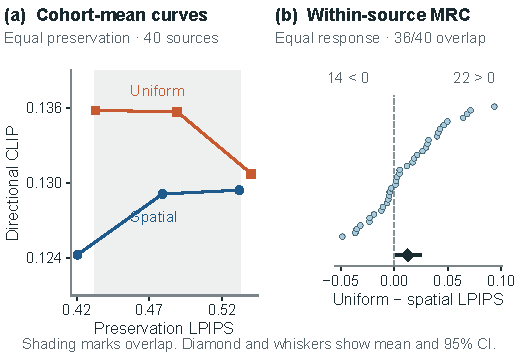
\includegraphics[width=\columnwidth]{figures/v19_aggregation.pdf}
\caption{Source-correction comparisons from three actual settings per arm. (a) Curves connect the three seed- and source-averaged operating points. At common preservation LPIPS the ordinate difference measures directional CLIP. (b) Each point is a source's interval-average preservation LPIPS difference at common directional CLIP, ordered vertically by value. Positive values favor spatial.}
\label{fig:v19-aggregation}\end{figure}
Figure~\ref{fig:v19-aggregation}(a) averages the two seeds and 40 sources for each of the three measured scales per allocation. Over their shared mean LPIPS range [0.43297, 0.53186], uniform minus spatial directional CLIP averages $+0.00652$ [0.00086, 0.01266] (20,000 archived source-bootstrap draws). The cohort-mean directional-CLIP ranges themselves are disjoint: spatial spans [0.12426, 0.12943] and uniform [0.13074, 0.13580].
Panel (b) instead pairs curves within source after averaging the two seeds at each setting. Thirty-six of 40 sources have positive-width directional-CLIP overlap. Of these, 22 favor spatial, 14 favor uniform, and none tie. Uniform minus spatial preservation LPIPS averages $+0.01280$ [0.00219, 0.02396], with median 0.00511. This comparison changes both the matching coordinate and the level at which shared support is constructed.

\subsection{Operating curves, pixel selectivity and edit categories}
\label{sec:v19-selectivity}
Each operating point averages the same 42 sources with a nonempty background.
Eight sources have a full edit mask and are excluded from all coordinates,
including directional CLIP. The 18 configurations give 756 source--output
pairs with positive background MAE and positive total change. Table~\ref{tab:v19-selectivity-points}
uses the five observed settings of each editor and three controls. The segments
in the operating plot follow knob order. Matched-response comparisons instead
use each source's own interval of directional CLIP overlap.

For source $i$, let $e_i$ and $b_i$ denote the mean absolute RGB changes per
edit and background pixel, and let $a_i$ be the fraction of pixels in the edit
mask. Whole-image MAE is $T_i=a_i e_i+(1-a_i)b_i$. Selectivity is
$s_i=e_i/b_i$ and the in-mask share of total change is
$\rho_i=a_i s_i/(1-a_i+a_i s_i)$. Each source contributes once to
$\bar s$ and $\bar\rho$. At scale 1.25, spatial SAM gives
$\bar s=4.8752$, $\bar e/\bar b=3.1998$ and median $s_i=3.8419$.
The mean source share is 0.5149 and the share of pooled change is 0.5219.
Table~\ref{tab:v19-selectivity-points} keeps the aggregation order explicit.

\begin{table*}[t]
\centering\small
\caption{All coordinates, including directional CLIP and selectivity, use the same 42 sources with background pixels. Main Table~1 reports directional CLIP on all 50. Background LPIPS uses either spatial feature-map averaging (FM) or masked inputs (MI). The pixel columns report mean whole-image MAE, the mean within-source ratio, the ratio of regional means and the mean within-source share. A star marks the native setting on each five-point curve.}
\label{tab:v19-selectivity-points}
\begin{tabular}{@{}lrrrrrrrr@{}}
\toprule
Configuration & Setting & LPIPS (FM) & LPIPS (MI) & Dir.\ CLIP & $\bar T$ & $\bar s$ & $\bar e/\bar b$ & $\bar\rho$\\
\midrule
Spatial & 0.25 & 0.0140 & 0.0091 & 0.0026 & 0.0132 & 2.0706 & 1.1961 & 0.3519 \\
Spatial & 0.50 & 0.0163 & 0.0107 & 0.0213 & 0.0149 & 2.4762 & 1.4480 & 0.3824 \\
Spatial & 0.75 & 0.0226 & 0.0148 & 0.0451 & 0.0187 & 3.1110 & 1.8887 & 0.4259 \\
Spatial & 1.00$^{*}$ & 0.0462 & 0.0297 & 0.0918 & 0.0283 & 4.0006 & 2.7419 & 0.4798 \\
Spatial & 1.25 & 0.1033 & 0.0593 & 0.1239 & 0.0458 & 4.8752 & 3.1998 & 0.5149 \\
\midrule
Uniform & 0.25 & 0.0156 & 0.0101 & 0.0047 & 0.0139 & 1.8813 & 1.1539 & 0.3436 \\
Uniform & 0.50 & 0.0239 & 0.0154 & 0.0227 & 0.0183 & 2.0542 & 1.2549 & 0.3559 \\
Uniform & 0.75 & 0.0498 & 0.0312 & 0.0457 & 0.0299 & 2.0018 & 1.3554 & 0.3644 \\
Uniform & 1.00$^{*}$ & 0.1656 & 0.0947 & 0.0950 & 0.0600 & 2.1079 & 1.5433 & 0.3795 \\
Uniform & 1.25 & 0.3268 & 0.2063 & 0.1235 & 0.1094 & 1.8753 & 1.4885 & 0.3782 \\
\midrule
FlowEdit & 12 & 0.0541 & 0.0340 & 0.0069 & 0.0222 & 2.1751 & 1.2694 & 0.3548 \\
FlowEdit & 16 & 0.0751 & 0.0478 & 0.0306 & 0.0284 & 2.6358 & 1.3289 & 0.3635 \\
FlowEdit & 20 & 0.1024 & 0.0664 & 0.0555 & 0.0365 & 3.0320 & 1.4193 & 0.3692 \\
FlowEdit & 24$^{*}$ & 0.1825 & 0.1185 & 0.0878 & 0.0602 & 2.5096 & 1.4755 & 0.3717 \\
FlowEdit & 28 & 0.5450 & 0.3546 & 0.1517 & 0.1996 & 1.8067 & 1.1493 & 0.3633 \\
\midrule
Two constants & --- & 0.0646 & 0.0416 & 0.0517 & 0.0344 & 2.0760 & 1.5423 & 0.3706 \\
Uniform @ S & --- & 0.0634 & 0.0423 & 0.0553 & 0.0343 & 2.0924 & 1.5379 & 0.3700 \\
Spatial @ U & --- & 0.1002 & 0.0552 & 0.1198 & 0.0460 & 4.9660 & 3.0792 & 0.5201 \\
\bottomrule
\end{tabular}
\end{table*}

From scale 0.25 to 1.25 the mean selectivity increase is 2.805 [1.717, 4.130]
for spatial SAM and $-0.006$ [$-0.477$, 0.396] for uniform SAM. The paired
difference between these increases is 2.811 [1.925, 3.917]. At scale 1.25
spatial SAM increases selectivity by 3.000 [2.114, 4.088] and the mean
in-mask share by 0.137 [0.099, 0.175] relative to uniform. Selectivity rises
on 37 of 42 sources. Spatial minus uniform directional CLIP is 0.0004
[$-0.0204$, 0.0202] at this setting, with 21 positive and 21 negative
differences. Background feature-map LPIPS is lower for spatial on all 42
sources, by 0.2235 [0.1851, 0.2634] on average.

At the default setting, two constants reduce whole-image MAE relative to
uniform by 0.0255 [0.0213, 0.0304]. Their mean selectivity difference is
$-0.032$ [$-0.147$, 0.083]. Uniform replay of the spatial profile gives
a mean selectivity of 2.092, close to the two-constant value of 2.076.
Spatial replay of the uniform profile gives 4.966, 2.858 [2.055, 3.846]
above native uniform. These intervals use 10,000 paired source bootstrap
draws with seed 0 and percentile endpoints. The contrasts measure changes
in pixels and text alignment under the specified settings.

\begin{table*}[t]
\centering\small
\caption{Matched uniform minus spatial background LPIPS by PIE-Bench edit category. The denominator counts sources with a background, and the numerator counts positive-width response overlaps. Both scorers give the same exceptions. Intervals resample sources within each row and are marginal 95\% intervals. A single style edit supplies a point estimate only.}
\label{tab:v19-selectivity-category}
\begin{tabular}{@{}lrrrrrr@{}}
\toprule
Edit category & Overlap & Negative & FM mean & FM interval & MI mean & MI interval\\
\midrule
Random & 4/4 & 0 & $0.0820$ & $[0.0143, 0.1496]$ & $0.0557$ & $[0.0066, 0.1378]$ \\
Replace & 5/5 & 1 & $0.0248$ & $[-0.0322, 0.0901]$ & $0.0239$ & $[-0.0054, 0.0629]$ \\
Add & 5/5 & 0 & $0.0526$ & $[0.0239, 0.0812]$ & $0.0207$ & $[0.0136, 0.0265]$ \\
Delete & 5/5 & 0 & $0.0482$ & $[0.0100, 0.0977]$ & $0.0451$ & $[0.0108, 0.0884]$ \\
Content & 4/4 & 0 & $0.0505$ & $[0.0341, 0.0618]$ & $0.0451$ & $[0.0303, 0.0560]$ \\
Pose & 4/4 & 2 & $0.0051$ & $[-0.0316, 0.0419]$ & $-0.0013$ & $[-0.0300, 0.0246]$ \\
Color & 5/5 & 0 & $0.0655$ & $[0.0246, 0.1067]$ & $0.0483$ & $[0.0185, 0.0784]$ \\
Material & 4/5 & 0 & $0.0211$ & $[0.0105, 0.0316]$ & $0.0131$ & $[0.0022, 0.0240]$ \\
Background & 4/4 & 1 & $0.0006$ & $[-0.2419, 0.1707]$ & $0.0474$ & $[-0.0024, 0.0973]$ \\
Style & 1/1 & 0 & $0.0086$ & --- & $0.0043$ & --- \\
\midrule
All & 41/42 & 4 & $0.0390$ & $[0.0106, 0.0632]$ & $0.0326$ & $[0.0204, 0.0462]$ \\
\bottomrule
\end{tabular}
\end{table*}

The feature-map and masked-input scorers agree on the sign of all 41 supported
uniform--spatial contrasts (Table~\ref{tab:v19-selectivity-category}).
Two of four pose edits favor uniform: changing a dog's posture from lying
down to jumping ($-0.0119$ feature-map LPIPS) and opening a closed lid
($-0.0514$). The other exceptions replace a mountain reflection with a
ship reflection ($-0.0674$) and change a rice-field background ($-0.3656$).
The pose means are 0.0051 and $-0.0013$ under feature-map and masked-input
scoring, respectively. Background edits have means of 0.0006 and 0.0474.
Category support ranges from one to five images. These summaries locate
the observed reversals and quantify their sensitivity to the scorer.

Across all supported sources, the mean FlowEdit-minus-spatial contrast is
0.1196 [0.0739, 0.1631] under feature-map scoring and 0.0905 [0.0625, 0.1227]
under masked-input scoring. All 38 source signs agree. For FlowEdit minus
uniform, the corresponding estimates are 0.0638 [0.0229, 0.1046] and
0.0489 [0.0220, 0.0790]. The scorers agree on 39 of 41 source signs.
Figure~\ref{fig:v19-response-sensitivity} gives the same-source default and matched
gaps, the three paired distributions and the mass-weighted localization plane.

\subsection{Matched response under alternative crossings, support, and weighting}
\label{sec:v20-mrc}
We use the same background feature-map LPIPS outcome in both studies. Let $d_i$ be the signed area between two preservation curves divided by their positive response-overlap width $w_i$ on source $i$. The primary estimate is the mean of $d_i$. Weighting by width gives $\sum_i w_i d_i/\sum_i w_i$, so a source spanning twice the response range receives twice the weight. Positive differences indicate lower background LPIPS for the subtracted arm.

\begin{table*}[t]
\centering\footnotesize
\caption{SAM matched-response sensitivity. Each estimate is a difference in background feature-map LPIPS with its marginal 95\% paired-source bootstrap interval. S, U and F denote spatial SAM, uniform SAM and FlowEdit. For the last two rows, $n$ counts sources contributing to the mean curves.}
\label{tab:v20-mrc}
\setlength{\tabcolsep}{3pt}
\begin{tabular}{@{}lrlrlrl@{}}
\hline
 & \multicolumn{2}{c}{U $-$ S} & \multicolumn{2}{c}{F $-$ S} & \multicolumn{2}{c}{F $-$ U}\\
Analysis & $n$ & Mean [95\% CI] & $n$ & Mean [95\% CI] & $n$ & Mean [95\% CI]\\
\hline
First crossing & 41 & $0.0390\;[0.0106,0.0632]$ & 38 & $0.1196\;[0.0739,0.1631]$ & 41 & $0.0638\;[0.0229,0.1046]$\\
Last crossing & 41 & $0.0457\;[0.0134,0.0729]$ & 38 & $0.1428\;[0.0919,0.1914]$ & 41 & $0.0761\;[0.0344,0.1196]$\\
Width weighted & 41 & $0.0696\;[0.0435,0.0946]$ & 38 & $0.1419\;[0.1000,0.1862]$ & 41 & $0.0663\;[0.0162,0.1159]$\\
Common sources & 38 & $0.0429\;[0.0124,0.0682]$ & 38 & $0.1196\;[0.0739,0.1631]$ & 38 & $0.0589\;[0.0167,0.1028]$\\
Common interval & 38 & $0.0467\;[0.0079,0.0797]$ & 38 & $0.1162\;[0.0700,0.1609]$ & 38 & $0.0695\;[0.0323,0.1084]$\\
Common interval, width weighted & 38 & $0.0707\;[0.0432,0.0981]$ & 38 & $0.1441\;[0.0970,0.1937]$ & 38 & $0.0734\;[0.0274,0.1176]$\\
Two prompts excluded & 39 & $0.0385\;[0.0087,0.0639]$ & 36 & $0.1161\;[0.0673,0.1621]$ & 39 & $0.0591\;[0.0175,0.1022]$\\
Edit MAE response & 42 & $0.0417\;[0.0227,0.0598]$ & 41 & $0.0834\;[0.0584,0.1092]$ & 42 & $0.0260\;[0.0089,0.0436]$\\
Mean curves, pair sources & 41 & $0.0758\;[0.0424,0.1006]$ & 38 & $0.1194\;[0.0722,0.1837]$ & 41 & $0.0387\;[-0.0020,0.0926]$\\
Mean curves, all eligible & 42 & $0.0744\;[0.0403,0.0993]$ & 42 & $0.1190\;[0.0732,0.1828]$ & 42 & $0.0426\;[0.0017,0.0990]$\\
\hline
\end{tabular}
\end{table*}

\paragraph{Coverage and integration.}
On SAM, 42 of 50 sources have a background. At first directional-CLIP crossing, 41, 38 and 41 have positive overlap for U$-$S, F$-$S and F$-$U, respectively. The median widths are 0.07594, 0.09204 and 0.09399 directional-CLIP units. In each case the remaining eligible sources have disjoint ranges. We connect the five observations in setting order, split the overlap at response knots, and integrate each linear piece. First and last crossing select the earliest and latest segments covering its midpoint. For the ambiguity check we omit sources \texttt{611000000001} and \texttt{812000000002}, leaving 40 background-eligible sources among 48. The MAE rows match the magnitude of RGB change within the edit mask.

\paragraph{Source set, interval and weighting.}
All three comparisons share 38 sources. On these sources, U$-$S is $+0.0429$ over each pair's own interval and $+0.0467$ over each source's three-arm interval. Changing only the interval shifts the estimate by $+0.0039$ $[-0.0087,0.0206]$. The three-arm intervals have median width 0.05298. Integrating every pair over those intervals gives additive contrasts within each source and in the means. On the primary 41 sources, weighting by pairwise width increases U$-$S by $+0.0306$ $[0.0129,0.0493]$; taking the last crossing changes it by $+0.0067$ $[-0.0023,0.0174]$. Computing the two cohort-mean curves first on those same 41 sources increases U$-$S by $+0.0368$ $[0.0062,0.0642]$.

\paragraph{Restoring operator.}
We first average seeds 0 and 17 at each of three measured scales (0.7, 1.0 and 1.3) for both allocations on the uniform-origin profile. At equal directional CLIP, 36 of 40 sources have positive overlap (median width 0.01286). Uniform minus request LPIPS is $+0.0128$ $[0.0022,0.0240]$ at first crossing, $+0.0178$ $[0.0061,0.0304]$ at last crossing and $+0.0121$ $[0.0012,0.0243]$ under width weighting. Matching edit MAE gives $+0.0308$ $[0.0197,0.0424]$ on 40 sources (median width 0.03184 MAE). Averaging the CLIP curves before matching gives disjoint ranges on all 40. On the 36 individually supported sources the mean curves overlap by 0.00032 CLIP, yielding $+0.0117$; 7,792 of 10,000 resamples support that estimate. The historical inverse comparison matches mean curves on background LPIPS and measures directional CLIP. Its 40-source uniform minus request CLIP difference is $+0.00652$ $[0.00086,0.01266]$ over LPIPS 0.43297 to 0.53186.

\paragraph{Uncertainty.}
The forward comparisons use 10,000 paired source resamples and percentile intervals. Each draw carries all settings and arms for a sampled source. We recompute width-weighted ratios and mean-curve overlaps in each draw. We report an interval when all draws support the estimate. For differences between estimators with different contributing sets, we resample their union and apply each estimator's inclusion rule to the same draw. The accompanying CSV also gives contrasts restricted to the source intersection. The historical inverse comparison retains its original 20,000 category-stratified source draws.

\subsection{What the restoring correction acts on}
% Supplement-only insertion; manuscript-relative figure path.
\begin{figure*}[t]
\centering
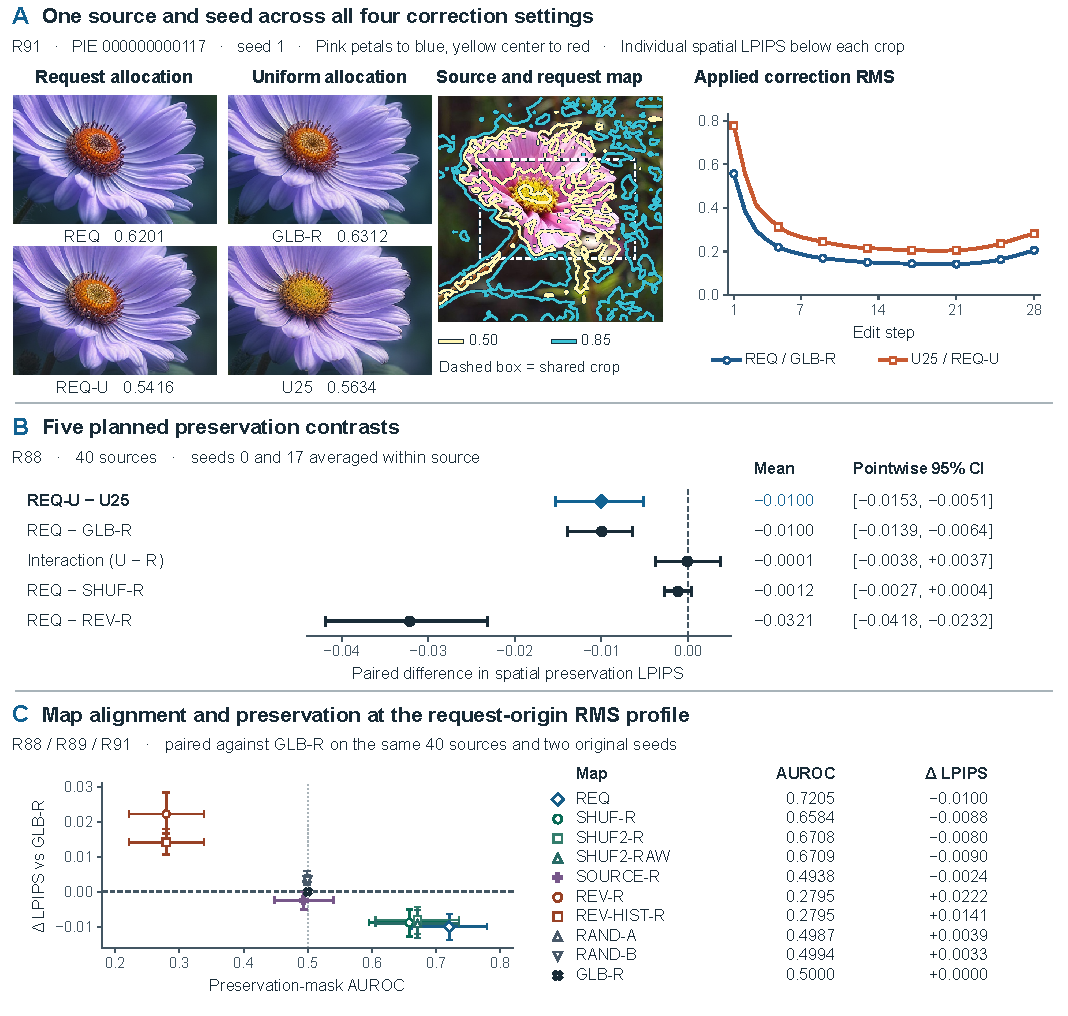
\includegraphics[width=.96\textwidth]{figures/v19_corrector_controls.pdf}
\caption{Source-corrector controls on the common spatial preservation LPIPS scale.
(A) All four native outputs use the same crop of a $512\times512$ image. Each score uses the complete preservation mask. The upper and lower rows use the request- and uniform-origin RMS profiles, respectively. Contours show two levels of the recorded request weight on the source. Lines trace the two native profiles, and open symbols mark every fourth replay step and the endpoint. The largest discrepancy over all 28 steps is $2.98\times10^{-8}$.
(B) The diamond marks the historical primary contrast. The historical interaction subtracts the request-profile allocation contrast from the uniform-profile contrast. Bars are the archived pointwise 95\% category-stratified paired-source bootstrap intervals.
(C) For each applied map, the abscissa gives the AUROC for predicting the official preservation mask. The ordinate gives the paired LPIPS difference from GLB-R, whose constant weights give AUROC 0.5. Negative differences favor the named map. Horizontal and vertical intervals are marginal 95\% category-stratified source bootstraps (20,000 draws). Each source contributes its mean over seeds 0 and 17.}
\label{fig:v19-corrector-controls}
\end{figure*}

The first shuffled donor (SHUF-R) gives a mean AUROC of 0.6584 and a preservation LPIPS difference of $-0.0088$ from GLB-R. The correct request map gives 0.7205 and $-0.0100$, respectively. The two reversed maps have nearly identical mean AUROC (0.2795) and different LPIPS penalties ($+0.0222$ and $+0.0141$). The protection-floor runs use the uniform-origin profile on 20 sources and are reported separately.

\begin{figure}[t]\centering
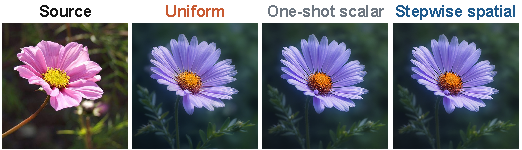
\includegraphics[width=\columnwidth]{figures/v19_restoring_flower_strip.pdf}
\caption{At seed 0 the three restoring configurations produce blue-violet petals and an orange center in response to a blue-flower, red-center request. The uniform, scalar-calibrated and spatial replay outputs are displayed at the same coordinates.}
\label{fig:v19-flower}\end{figure}

\subsection{How editing papers evaluate spatial components}
\paragraph{Selection and access.} On 19 November 2026, two AI agents independently coded disjoint, prespecified lists of 12 papers each. The papers were selected by title from the design review and its bibliography to cover regional controls and related inversion, feature-injection and whole-image methods published or posted in 2023--2026. The second list records one year-based exclusion (Blended Diffusion, CVPR 2022) and its replacement (PnP Inversion, ICLR 2024). Blended Latent Diffusion is a separate, in-period paper. For each title the recorded trail identifies a proceedings, publisher or author-version paper, its comparison site and the figure, table or section inspected. Each paper received one machine assessment. The audit records no human ratings or inter-rater agreement estimate. Counts refer to this purposive sample.

\paragraph{Eligibility and coding.} A regional comparison changes spatial support, weighting or its construction within a method. Of the 24 papers, 15 document such a comparison, two leave eligibility unclear, one tests whole-field feature injection and six concern other control sites. The last nine are listed separately. For the 15 eligible papers, the toggle criterion asks whether the design identifies an on/off comparison at a specified setting. The first sheet coded a specified default toggle. The second asked whether the comparison was a single default toggle. Thus DirectEdit's multi-setting design receives N for this field even though it includes a mask-off arm. Eight papers left the fixed-setting design unclear. A norm match requires evidence that the two regional arms equalize the measured norm of the same gated update. Matching a coefficient or the mean gate alone does not meet this criterion. A response comparison must align achieved edit response or trace a response--preservation curve for those arms. Two output scores at one setting supply one operating point.

\paragraph{Evidence decisions.} Y requires a qualifying comparison in the cited material. Sheet A used N when inspection found no qualifying control. Sheet B used N for a design that failed a criterion and NR when the control was unreported. The tables retain those codes. A question mark records unresolved design or access, O an out-of-scope site, and n/a an inapplicable field. When experiments in one paper address different interventions, the code follows the named comparator. ASG Table~3(c) replaces each spatial gate by its per-image mean, matching a gate statistic. DecFlowEdit Fig.~7 compares its spatial and uniform configurations at comparable edited-region CLIP. Its Table~9 matches the realized norms of two CFG directions on the same current state. CPR crosses profiles recorded on two native trajectories. DiffEdit, DecFlowEdit, InstantEdit and DirectEdit meet the response criterion, which includes cohort curves and approximate response calibration.

Paper titles below link to the source inspected, with PDF page numbers where available. Full papers were available for 23 titles, with appendix or supplementary evidence where recorded. For Peng et al.'s ICME FlowEdit, the accessible publisher record comprised the abstract, section list and supplemental-item listing. The full PDF and listed ZIP were inaccessible. Its four fields remain unclear.

\begin{table*}[t]\centering\small
\caption{The 15 papers with a documented regional comparison. R = regional comparison, T = fixed-setting toggle, M = same-term norm match, and A = output-response alignment or curve.}
{\setlength{\tabcolsep}{3pt}\begin{tabularx}{\textwidth}{@{}p{.21\textwidth}X p{.25\textwidth}cccc@{}}\toprule
Paper & Intervention or comparator & Primary-source location & R & T & M & A\\\midrule
\href{https://openreview.net/pdf?id=3lge0p5o-M-}{DiffEdit} & Mask vs. encode--decode & Figs.~5--6, p.~7 and App.~A.4, pp.~15--16 & Y & ? & N & Y\\
\href{https://openaccess.thecvf.com/content/ICCV2023/papers/Cao_MasaCtrl_Tuning-Free_Mutual_Self-Attention_Control_for_Consistent_Image_Synthesis_and_ICCV_2023_paper.pdf}{MasaCtrl} & Unrestricted vs. mask-guided attention & Figs.~2, 9, pp.~2, 9 & Y & Y & N & N\\
\href{https://openaccess.thecvf.com/content/ICCV2025/papers/Zhu_KV-Edit_Training-Free_Image_Editing_for_Precise_Background_Preservation_ICCV_2025_paper.pdf}{KV-Edit} & Inversion attention mask on/off & Table~2 and Fig.~7, pp.~7--8 & Y & ? & N & N\\
\href{https://arxiv.org/pdf/2609.34237v1}{DecFlowEdit} & Spatial vs. uniform update scaling & App.~D.1, Fig.~7, pp.~16--17 and App.~E.4, Table~9, p.~21 & Y & ? & N & Y\\
\href{https://arxiv.org/pdf/2603.13388v1}{VeloEdit} & Velocity-replacement threshold & Tables~4--5, p.~10 & Y & ? & N & N\\
\href{https://openaccess.thecvf.com/content/ICCV2025/papers/Gong_InstantEdit_Text-Guided_Few-Step_Image_Editing_with_Piecewise_Rectified_Flow_ICCV_2025_paper.pdf}{InstantEdit} & Mask on/off in disentangled guidance & Table~4, p.~8 and \href{https://openaccess.thecvf.com/content/ICCV2025/supplemental/Gong_InstantEdit_Text-Guided_Few-Step_ICCV_2025_supplemental.pdf}{supp.\ B, p.~1} & Y & ? & N & Y\\
\href{https://openaccess.thecvf.com/content/ICCV2025/papers/Patel_FlowChef_Steering_of_Rectified_Flow_Models_for_Controlled_Generations_ICCV_2025_paper.pdf}{FlowChef} & Predicted vs. annotated edit mask & Table~4 and Fig.~5, p.~8 & Y & ? & N & N\\
\href{https://arxiv.org/pdf/2606.06228v1}{SAM-Flow} & Soft support, ring and accumulation & Fig.~6, pp.~8--9 and App.~G, pp.~16--18 & Y & ? & N & N\\
\href{https://arxiv.org/pdf/2609.37492v1}{Attention-scoped Guidance} & Attention gates vs. uniform CFG & Tables~2 and 3(c), p.~4 & Y & Y & N & N\\
\href{https://arxiv.org/pdf/2206.02779v2}{Blended Latent Diffusion} & Static vs. shrinking mask & Figs.~6--7, p.~6 and App.~C, pp.~12--13 & Y & Y & N & N\\
\href{https://www.ecva.net/papers/eccv_2024/papers_ECCV/papers/02585.pdf}{RegionDrag} & Density of region-derived point pairs & Figs.~7--8, pp.~13--14 & Y & N & NR & NR\\
\href{https://openaccess.thecvf.com/content/CVPR2026/papers/Bradbury_Your_Latent_Mask_is_Wrong_Pixel-Equivalent_Latent_Compositing_for_Diffusion_CVPR_2026_paper.pdf}{Pixel-Equivalent Latent Compositing} & LoRA with/without the compositor & Table~3, p.~7 & Y & Y & NR & NR\\
\href{https://raw.githubusercontent.com/mlresearch/v306/main/assets/yang26cy/yang26cy.pdf}{DirectEdit} & Noise blending with/without a mask & Table~1 and Fig.~5, p.~7 & Y & N & NR & Y\\
\href{https://proceedings.neurips.cc/paper_files/paper/2023/file/3469b211b829b39d2b0cfd3b880a869c-Paper-Conference.pdf}{Diffusion Self-Guidance} & Weights on object-shape guidance & App.~C, Figs.~16--17, pp.~17--18 & Y & N & NR & NR\\
\href{https://arxiv.org/pdf/2302.03027}{Pix2Pix-Zero} & Cross-attention discrepancy guidance on/off & Fig.~6 and Table~2, pp.~8--10 & Y & ? & NR & NR\\
\bottomrule\end{tabularx}}
\end{table*}

\begin{table*}[t]\centering\small
\caption{The other nine selected papers, excluded from the regional-control counts. R = regional comparison, T = fixed-setting toggle, M = same-term norm match, and A = output-response alignment or curve.}
{\setlength{\tabcolsep}{3pt}\begin{tabularx}{\textwidth}{@{}p{.21\textwidth}X p{.25\textwidth}cccc@{}}\toprule
Paper & Intervention or comparator & Primary-source location & R & T & M & A\\\midrule
\href{https://openreview.net/pdf?id=_CDixzkzeyb}{Prompt-to-Prompt} & Injection duration and optional local blending & Fig.~5, p.~6 and App.\ Fig.~21, p.~26 & ? & ? & N & N\\
\href{https://openaccess.thecvf.com/content/CVPR2023/papers/Tumanyan_Plug-and-Play_Diffusion_Features_for_Text-Driven_Image-to-Image_Translation_CVPR_2023_paper.pdf}{Plug-and-Play Diffusion Features} & Whole-field feature/attention injection & Fig.~9(a) and Sec.~5.2, pp.~7--8 & N & ? & N & N\\
\href{https://openaccess.thecvf.com/content/CVPR2025/papers/Avrahami_Stable_Flow_Vital_Layers_for_Training-Free_Image_Editing_CVPR_2025_paper.pdf}{Stable Flow} & Choice of feature-injection layers & Sec.~4.3 and Table~2, pp.~6--8 & O & n/a & n/a & n/a\\
\href{https://raw.githubusercontent.com/mlresearch/v267/main/assets/wang25ce/wang25ce.pdf}{RF-Edit / RF-Solver} & Source value sharing over steps & Fig.~7 and Table~5, pp.~5, 8 & O & n/a & n/a & n/a\\
\href{https://raw.githubusercontent.com/mlresearch/v267/main/assets/deng25c/deng25c.pdf}{FireFlow} & Cached inversion values and step count & App.~A, p.~12 and Fig.~8, pp.~16--17 & O & n/a & n/a & n/a\\
\href{https://ieeexplore.ieee.org/document/11209009}{FlowEdit (Peng, ICME)} & Attention control mentioned in abstract & IEEE 11209009, abstract and item listing & ? & ? & ? & ?\\
\href{https://openaccess.thecvf.com/content/CVPR2023/papers/Kawar_Imagic_Text-Based_Real_Image_Editing_With_Diffusion_Models_CVPR_2023_paper.pdf}{Imagic} & Text interpolation and fine-tuning & Figs.~7--9, pp.~7--8 & O & n/a & n/a & n/a\\
\href{https://openaccess.thecvf.com/content/CVPR2023/papers/Mokady_NULL-Text_Inversion_for_Editing_Real_Images_Using_Guided_Diffusion_Models_CVPR_2023_paper.pdf}{Null-text Inversion} & Inversion and null-embedding optimization & Figs.~4--5, 7, pp.~6--7 & O & n/a & n/a & n/a\\
\href{https://proceedings.iclr.cc/paper_files/paper/2024/file/661caac7729aa7d8c6b8ac0d39ccbc6a-Paper-Conference.pdf}{PnP Inversion} & Branch corrections and guidance scale & Tables~4--5, p.~9 and App.~E.4, p.~19 & O & n/a & n/a & n/a\\
\bottomrule\end{tabularx}}
\end{table*}

\subsection{Instruction-success rating design}
The default configurations supply 150 comparisons (50 sources each under spatial allocation, uniform allocation and the two-constant control). In each comparison a rater sees the source, the requested edit and one full-resolution output. Raters answer whether the requested visible change appeared, using a binary response. The output configuration is concealed. Each rater receives a separate randomized order and opaque item identifiers. Clarifications for two conflicting benchmark descriptions follow the source-to-target prompt transition used to generate the image and are identical across configurations. Optional uncertainty flags are retained separately from the binary answer.
 
The design pairs the same 150 outputs across independent raters. The scoring script reports success counts and rates by configuration and agreement on items rated in common. For formal comparisons all three configurations use the same sources with complete ratings. Rates average raters within source. Differences and intervals use paired resampling of sources (10,000 draws); the scoring guide specifies missing-item and agreement rules before collection. With two complete independent exports it calculates Cohen's $\kappa$; with three it also calculates Fleiss' $\kappa$. No completed human evaluation is available. Directional CLIP and pixel concentration in the paper measure embedding response and the location of change, respectively.

\subsection{How individual examples were selected}
We chose the shirt, helmeted dog and jar in main Fig.~3 after inspecting the outputs. Their requests change a color, add flowers to the dog's mouth and open a lid, respectively. Figure~\ref{fig:v19-ranked-changes} separately retains the original example-selection rule. It ranks all 50 sources on two contrasts in directional CLIP (uniform minus constants and spatial minus constants) and selects cases near high, middle and low joint ranks. The painting has a full edit mask. Its background score is undefined, whereas its embedding response and whole-image change are measurable.

\begin{figure*}[t]\centering
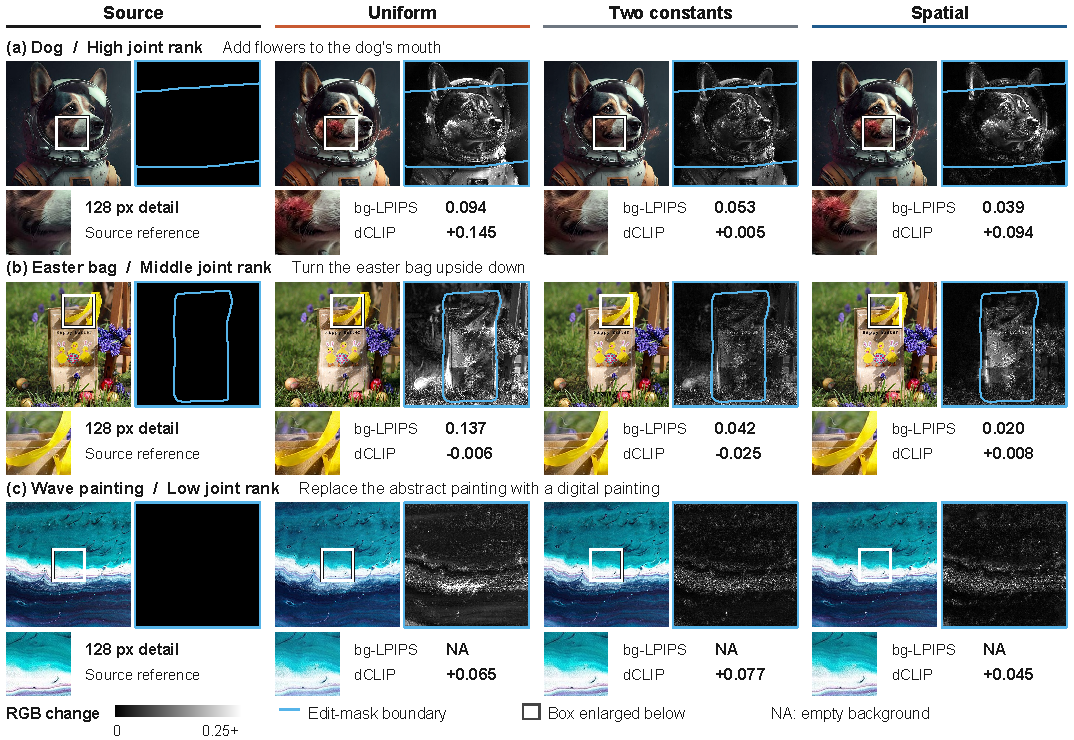
\includegraphics[width=\textwidth]{figures/v19_changes_ranked.pdf}
\caption{A high joint-rank dog, a middle-rank bag and a low-rank painting under the original selection rule. The bag stays upright under all three configurations. Scores beside the crops are regional feature-map LPIPS and directional CLIP. All maps share the same absolute RGB scale across images and configurations.}
\label{fig:v19-ranked-changes}
\end{figure*}
\begin{figure*}[t]\centering
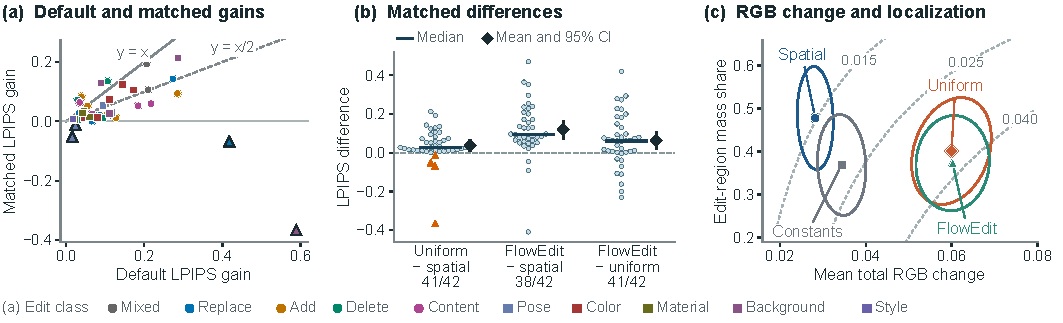
\includegraphics[width=\textwidth]{figures/v19_response.pdf}
\caption{The size of the response-matching adjustment varies by source. Panel (a) pairs default and matched gaps within each image. Panel (b) shows all three configuration contrasts. The last panel shows total pixel change and its concentration on the 42 nonempty backgrounds. The common spatial LPIPS field supplies the background measure throughout.}
\label{fig:v19-response-sensitivity}
\end{figure*}

\section{SAM-Flow: From Native Gains to Equal Editing Response}
\label{sec:sam}
This section reports the prespecified SAM analyses with masked-input (MI) LPIPS. The main paper uses the feature-map (FM) measure for both operators. At its default setting, spatial SAM-Flow reduces background LPIPS by 0.06496 relative to the same editor with uniform projection. Two constants calibrated on the native trajectory recover 81.7\% of that reduction (95\% CI 77.0--86.1\%), while reducing directional CLIP by 0.04054 relative to uniform. Across all five measured settings at matched directional CLIP, spatial SAM retains a background advantage of $\ScanSUMean$ [$\ScanSULo,\ScanSUHi$] on $\ScanSUValid$ sources with overlapping responses. These quantities compare a default configuration, a change to its projection, and an operating point selected for the same measured edit response.

\subsection{Sources, prompts and regional scores}
We sampled five PIE-Bench sources in each of ten editing categories. Within category the sampling key was the SHA-256 digest of \texttt{A-dose-lens-pilot-20261117-v1:} followed by the 12-digit source ID. Selection used the 700-entry benchmark and preceded outcome scoring. The 50 selected images share neither IDs nor decoded RGB images with the 40-source primary correction cohort. Two development IDs recur, one from each earlier pilot (Section~\ref{sec:development}). Sources with global edits remain in the sample. In category order 0--9, the counts with a nonempty preservation region are $4,5,5,5,4,4,5,5,4,1$. All 50 have an edit region.

The editor received the recorded source and target prompts with the benchmark's annotation brackets removed. Token selection used the text spans and, in 20 cases, manually supplied context tokens identifying the affected noun or phrase. The source and a FlowEdit scout supply attention maps. Benchmark evaluation masks enter scoring only. Two discrepancies surfaced in the visual audit. The raw instruction for 611000000001 refers to a raven, while its image and model prompts concern an otter and colored hearts. For 812000000002 the raw instruction places a house in front of the girl, while the target prompt places the girl in front of a house. We retained both original model inputs and both sources throughout the prespecified analysis.

Given the binary edit mask $M_{\rm edit}$ on the $512\times512$ grid, the preservation mask is $B=1-M_{\rm edit}$. We multiply both RGB images in $[0,1]$ by $B$, convert to $[-1,1]$, and evaluate the learned AlexNet-v0.1 LPIPS scalar on the resulting full images. Black pixels replace the edit region before feature extraction. The scalar uses the network's spatial averaging without division by background area. The separate source-correction study weights an LPIPS \emph{distance map} computed on intact images. We compare LPIPS differences within the corresponding study.

Directional CLIP is the cosine between the change in unit-normalized CLIP ViT-B/32 image embeddings (output minus source) and the change in unit-normalized text embeddings (target minus source prompt). The image processor uses its 224-pixel input. A zero-norm embedding difference has undefined cosine. Edit-region MAE is the sum of RGB absolute differences in $[0,1]$ over $M_{\rm edit}$ divided by three times its pixel count. Empty support has a missing regional score. Background summaries therefore use 42 sources, and directional CLIP and edit-region MAE use all 50. Every output contributes to each score for which it has support. MAE quantifies change in the edit region, including changes to the wrong object.

\subsection{Projection, allocation and the two constants}
The published FLUX implementation of SAM-Flow~\cite{cui2026sam} is pinned to commit \path{8167978666e6df11e987a453934b89ec422bd3a4}. All arms share the FLUX.1-dev backbone, source, prompts, resolution, and generation seed 0 within source. The runner resets the generation seed for the shared scout and before each editing arm, pairing the draws for latent sampling and forward noise across the compared configurations. A separate seed, 999, controls the attention-reference noise. All five settings use the same generation seed on each source. The grid has 28 steps, SAM uses 26 active steps and eight noise averages. Its source/target guidance scales are 1.5/10.5. The independent FlowEdit reference~\cite{kulikov2025flowedit} uses its native differential update with target guidance 5.5 and default $n_{\max}=24$.

Let $A$ be the source anchor and $R_i=z_i^{\rm full}-A$ the accumulated proposed displacement. The model and visible states receive $A+P_i^k\odot R_i$, for branch $k=m,v$. With projection scale $\alpha$, native soft and hard gates $W_s,W_h$, core weight $C$, and ring-only weight $J$, the implemented factors are
\begin{align}
P_i^m &= \alpha W_s, &
P_i^v &= \alpha(CW_s+0.35\,J W_h).
\end{align}
The visible branch uses the original core/ring blending order. Uniform uses the same scalar at every location in both branches. Both arms retain the scout and prompt processing. Define $b_i^k=\RMS(P_i^k\odot R_i)$ over all latent coordinates. These are displacements after the Euler update, with the 26 active steps weighted equally. For the older velocity correction we integrate RMS with the step size $h_i$. Stronger projection here permits greater departure from the source. Stronger additive protection in the correction editor pushes the state toward the source.

For each source the constant comparator computes $p_k=\sum_i b_i^k/\sum_i\RMS(R_i)$ on the native spatial trajectory. It then applies $p_k$ at every location and step in its own rollout. The two fitted constants depend only on the reference profile. On the resulting trajectory the summed FP32 projection magnitude exceeds native by 8.42\% on average.

\begin{table}[!t]
\centering\footnotesize
\caption{SAM controls and the FlowEdit reference on 50 sources. Background LPIPS uses the original masked-input (MI) score on the 42 with a preservation region. $S$ and $U$ denote the native spatial and uniform profile origins.}
\label{tab:sam-core}
\begin{tabular}{@{}lrrr@{}}\toprule
Configuration & BG LPIPS & Dir.\ CLIP & Edit MAE\\\midrule
FlowEdit 24 & .1185 & .0842 & .0861\\
Native spatial & .0297 & .0841 & .0587\\
Uniform & .0947 & .0927 & .0863\\
Two constants & .0416 & .0521 & .0493\\
Uniform at $S$ & .0423 & .0546 & .0490\\
Spatial at $U$ & .0552 & .1100 & .0997\\\bottomrule
\end{tabular}
\end{table}
The recovery fraction is the ratio of two paired cohort-mean gains, $0.05310/0.06496$. Core uncertainty uses 20,000 paired source bootstrap draws (seed 20261118), recomputing the ratio in each draw. Relative to uniform, the two constants change directional CLIP by $-0.04054$ [$-0.05709,-0.02526$]. Relative to the constants, native spatial improves background LPIPS by $0.01186$ [0.00803, 0.01628] and increases directional CLIP by $0.03194$ [0.01485, 0.05031]. The CLIP increase is $0.04007$ [0.02123, 0.06039] on the same 42 sources that contribute LPIPS.

\subsection{Three default examples selected by directional CLIP}
\label{sec:sam-ranked}
Figure~\ref{fig:sam-ranked} shows the three rank-selected cases (dog, bag and painting). The dog also appears in main Fig.~3(b). To select the rows post hoc, we ranked all 50 sources independently on two directional-CLIP differences: uniform minus two constants and native spatial minus two constants. On each axis we divided the zero-based rank by 49, assigning tied scores their average rank. For the favorable, typical and contrary rows, respectively, we selected the point at the smallest Euclidean distance from $(0.9,0.9)$, $(0.5,0.5)$ and $(0.1,0.1)$. The favorable row required both differences to be positive and the contrary row required both to be negative. The typical row used all 50 sources. Equal distances were resolved by the lowest source ID.

For the dog (211000000000), the two directional-CLIP differences are $+0.1402$ and $+0.0888$, in uniform, then native spatial order. Both favor the corresponding default over the two-constant control. For the bag (524000000004) the differences are $+0.0190$ and $+0.0328$, yet all three outputs leave the bag upright. For the abstract-to-digital painting (000000000103), the differences are $-0.0122$ and $-0.0314$. Here the two-constant control has the highest directional CLIP.

\begin{figure*}[!t]
\centering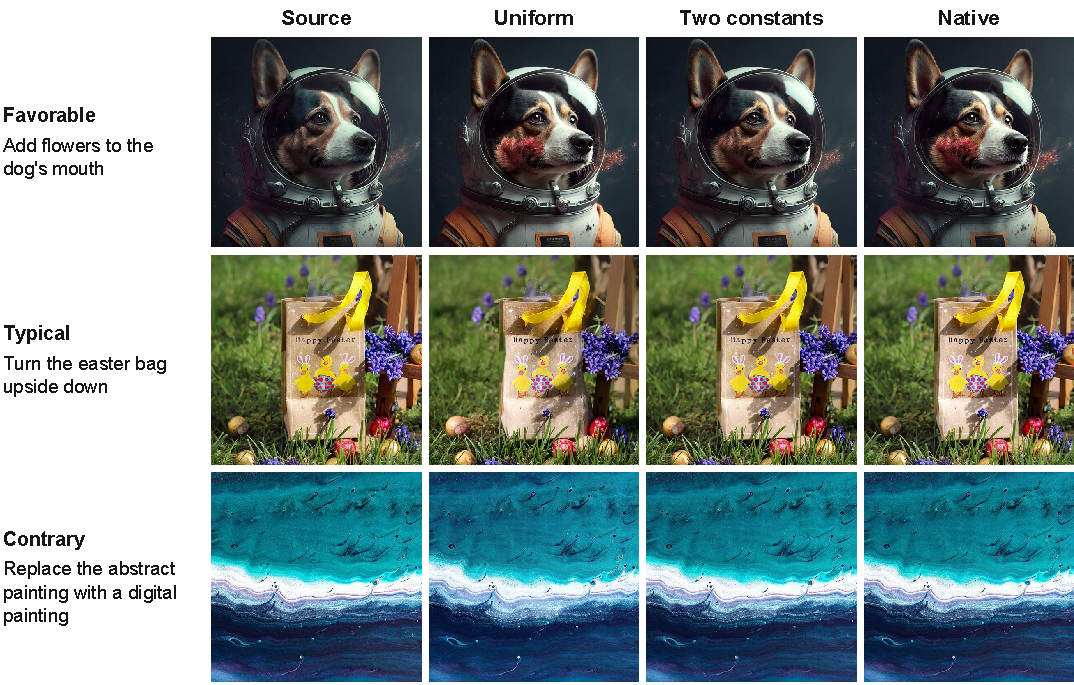
\includegraphics[width=\textwidth]{supp_sam_examples.pdf}
\caption{Three default SAM-Flow comparisons selected by the joint ranks of two directional-CLIP contrasts. Each row pairs the source with the uniform, two-constant and native spatial outputs at seed 0. All four views retain the full $512\times512$ field. The high-ranked dog shows color beside its muzzle; flowers held in its mouth are difficult to discern, the typical bag remains upright, and the contrary painting yields a higher text-response score under two constants than under either other setting.}
\label{fig:sam-ranked}
\end{figure*}

\subsection{Crossing the two measured projection profiles}
At every active step, replay recomputes the candidate direction on its own state and scales its RMS to the prescribed branch target. A zero target returns zero displacement. A positive target requires a nonzero candidate norm. At the spatial-origin profile, spatial minus uniform changes masked-input background LPIPS (MI) by $-0.01258$ [$-0.01673,-0.00894$] and directional CLIP by $+0.02947$ [0.01172, 0.04866]. At the uniform origin these contrasts are $-0.03950$ [$-0.05064,-0.02950$] and $+0.01738$ [$-0.00458,0.03979$]. The latter CLIP contrast on the 42 preservation-eligible sources is $+0.02485$ [0.00048, 0.04956].

The four MI-LPIPS cells yield two paths through the same native difference. Changing allocation at the spatial origin contributes $-0.01258$, and changing profile along the uniform allocation contributes $-0.05238$. Changing profile along the spatial allocation contributes $-0.02545$, and changing allocation at the uniform origin contributes $-0.03950$. Both paths give $-0.064957$ to six decimals when computed from unrounded cells. The post hoc CPR interaction in MI-LPIPS (allocation contrast at $S$ minus that at $U$) is $+0.02693$ [0.01856, 0.03631], positive on 41/42 sources (20,000 paired source resamples, seed 1208). The two historical source-correction paths appear in Table~\ref{tab:paths}.

Both branches at all 26 steps pass the pre-cast FP32 tolerance $10^{-6}+10^{-4}b_i^k$ in 100/100 replay runs. Comparing realized source-relative BF16 states after casting, with tolerance $10^{-6}+0.01b_i^k$, gives all-step passes in 3/50 uniform-at-spatial and 34/50 spatial-at-uniform runs. The largest single-step relative error is 11.39\%. The largest source/branch sum of absolute errors divided by the sum of its target RMS values is 0.336\%.

Replaying a target can take a blend outside the native convex range. We measured the effective coefficient as replay gain times the native factor at each location for spatial allocation, and as the gain itself for uniform allocation. At least one coefficient exceeded $1+10^{-6}$ in both branches of all 50 spatial-at-uniform runs (model maximum 2.04984, visible maximum 4.73960). Under uniform-at-spatial, 2/50 model branches exceeded the threshold (maximum 1.00847) and 0/50 visible branches did (maximum 0.95588). Replay retains these coefficients to prescribe the requested magnitude. At the measured scale $\alpha=1.25$, all 50 sources reached effective factors above one on both branches of both scanned arms, at each of the 26 active steps. For spatial gates the exceedance is a maximum over locations. The four scales through the default $\alpha=1$ stayed within the convex range. The archive provides per-source extrema in \path{analysis/v21_bounded/gate_ranges.csv}.

\subsection{Response-matched scan and coverage}
\label{sec:sam-scan}
Each source has five settings per arm. Native spatial varies its scale and uniform varies its uniform factor over $\{0.25,0.5,0.75,1,1.25\}$. FlowEdit varies $n_{\max}$ over $\{12,16,20,24,28\}$. The 750 curve points include 150 reused defaults and 600 additional outputs. The three remaining core controls contribute 150 distinct outputs, bringing the archive to 900/900 completed jobs. Figure~\ref{fig:sam-scan}(A) follows the response of each source across the five settings. Table~\ref{tab:sam-points} summarizes each setting across sources.

\begin{table}[!t]
\centering\scriptsize\setlength{\tabcolsep}{2.7pt}
\caption{Five settings per arm. Background LPIPS uses masked inputs (MI). Each row summarizes the observed images at one setting. Stars mark the three defaults.}
\label{tab:sam-points}
\begin{tabular}{@{}lrrrrrr@{}}\toprule
 & &\multicolumn{3}{c}{Directional CLIP}&\multicolumn{2}{c}{BG LPIPS}\\
Arm & Knob & $n$ & Mean & Median & $n$ & Mean\\\midrule
\ScanPointRows
\bottomrule\end{tabular}
\end{table}

For each source and arm, connect adjacent observed $(x,L)$ pairs in increasing knob order, where $x$ is directional CLIP and $L$ is preservation LPIPS. At a response with several crossings, take the earliest segment in knob order. For a vertical segment use the first endpoint. Each comparison requires all five finite pairs in both arms. Its lower endpoint $a$ is the larger of the two minimum responses, and $b$ is the smaller maximum. A separated range ($b<a$) or a single point ($b=a$) contributes to coverage only. When $b>a$, evaluate
\begin{equation}
d_j=(b-a)^{-1}\int_a^b [L_{\rm first\ arm}(x)-L_{\rm second\ arm}(x)]\,dx .
\end{equation}
Split the interval at all response knots in either curve. Midpoint evaluation on each subinterval integrates the selected affine branches exactly. Each valid source receives equal weight regardless of its interval width. We bootstrap the mean of these paired differences 10,000 times, resampling valid sources with replacement in ascending-ID order (PCG64, seed 0 restarted for each pair, linear percentile endpoints). The intervals are conditional on observed common support.

\begin{figure*}[!t]
\centering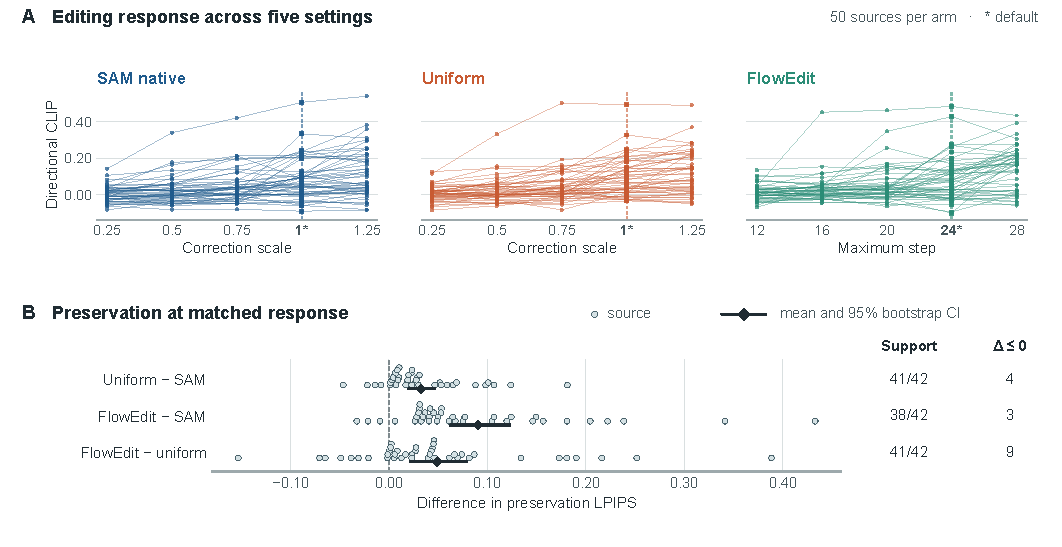
\includegraphics[width=\textwidth]{figures/scan_profile.pdf}
\caption{Five measured settings and paired masked-input background LPIPS (MI) at equal directional CLIP. (A) Each line follows one of 50 sources in knob order. The SAM scale sets the native spatial projection strength or the uniform projection factor. FlowEdit varies its maximum step. Stars mark the defaults. (B) Each dot is one source's interval-average background LPIPS difference over its pair's shared response range. Diamonds give equal-source means and bars show 95\% paired bootstrap intervals. A positive value favors the second named arm. Support is the number with positive-width overlap among the 42 sources with a background. The last column counts nonpositive differences.}
\label{fig:sam-scan}
\end{figure*}

\begin{table*}[!t]
\centering\small
\caption{Prespecified first-crossing analysis. ``Missing/disjoint/touch'' counts are among the 42 preservation-eligible sources. Width is median common directional-CLIP width. Differences are in background LPIPS. Positive favors the second named arm.}
\label{tab:sam-support}
\begin{tabular}{@{}lcrrrrrr@{}}\toprule
Contrast & Valid/eligible & Missing/disjoint/touch & Width & Mean & 95\% CI & Median & $d_j\leq0$\\\midrule
\ScanPairRows
\bottomrule\end{tabular}
\end{table*}
In Fig.~\ref{fig:sam-scan}(B) and Table~\ref{tab:sam-support}, the primary contrast is uniform minus native spatial. $\ScanSUPositive$ of $\ScanSUValid$ source differences are positive, four are negative, and source 712000000004 has disjoint response ranges. At the defaults, the mean difference on those same 41 sources is 0.0658. For the two secondary comparisons, FlowEdit minus spatial is positive on 35/38 sources and FlowEdit minus uniform on 32/41. Each comparison uses its own common response range and source set.

\subsection{Sensitivity and held-out prediction}
Switching to the last crossing changes the primary mean to $+0.03812$ [0.02431, 0.05300] (35 positive, 41 valid). Using edit-region MAE as the response gives $+0.03619$ [0.02420, 0.04959] (36 positive, 42 valid, median common width 0.07834 MAE). Excluding the two prompt discrepancies identified in the atlas gives $+0.03223$ [0.01918, 0.04671] with 35 positive among 39 overlapping sources (48 retained, 40 preservation-eligible, one disjoint). These are post hoc changes to the response definition, crossing convention or sample. The primary result retains both flagged sources and uses first crossing at equal directional CLIP.

A separate post hoc prediction targets the default background LPIPS reduction, uniform minus spatial. For each of the 42 eligible sources we fit ordinary least squares on the other 41. An intercept alone yields held-out RMSE/MAE 0.05104/0.03975. Background area fraction gives 0.05011/0.03930. Adding $1-\bar b^v_S/\bar b^v_U$, the relative attenuation in mean visible projected RMS across the two default rollouts, gives 0.04630/0.03401. The extra predictor thus uses information from running both default configurations on the held-out image. The validation population is the SAM cohort.

\subsection{Recorded execution cost}
A single RTX 4080 SUPER ran BF16 inference with model CPU offload (PyTorch 2.8.0+cu128, Diffusers 0.35.1, Transformers 4.56.2). The 300 core scientific jobs sum to 12.38 hours and 125,468 transformer evaluations. A resumed run reused 245 completed jobs and finished 55. The 600 additional scientific jobs sum to 22.52 hours and 229,800 evaluations: 200 native jobs took 9.43 hours/85,800 evaluations, 200 uniform jobs took 7.42 hours/83,200 evaluations, and 200 FlowEdit jobs took 5.67 hours/60,800 evaluations. Total recorded job time is 34.89 hours with 355,268 evaluations. Job times exclude failed launches, engineering checks, idle intervals and separate metric evaluation.

\subsection{Eight cases from the complete visual atlas}
Figures~\ref{fig:sam-cases1} and~\ref{fig:sam-cases2} show eight sources chosen after inspecting all 18 outputs for each of the 50 sources in ascending ID order. The examples show incomplete edits, changes to subject identity or viewpoint, and two discrepancies between the instruction and the model prompt. Each image shows the full field of view at seed 0. The upright bag also appears in the independently ranked default examples in Fig.~\ref{fig:sam-ranked}.

\begin{figure*}[!t]
\centering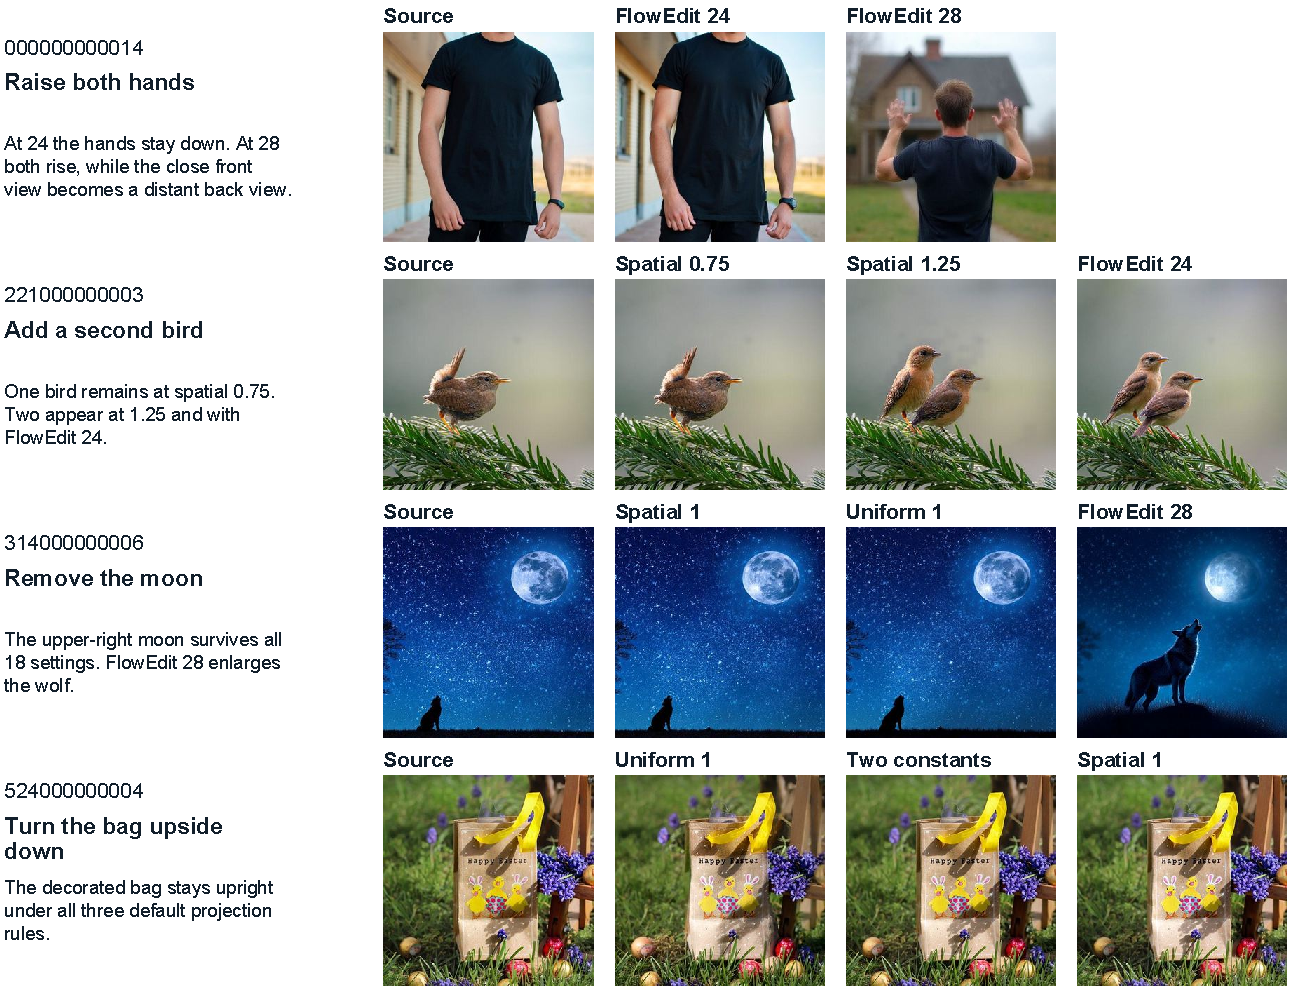
\includegraphics[width=.94\textwidth]{supp_cases_1.pdf}
\caption{Editing strength and requested geometric changes. Labels identify the actual source and control setting. The bird edit succeeds at the higher spatial setting. The bag stays upright at each displayed default, and the wolf retains the moon in all 18 outputs.}
\label{fig:sam-cases1}
\end{figure*}
\begin{figure*}[!t]
\centering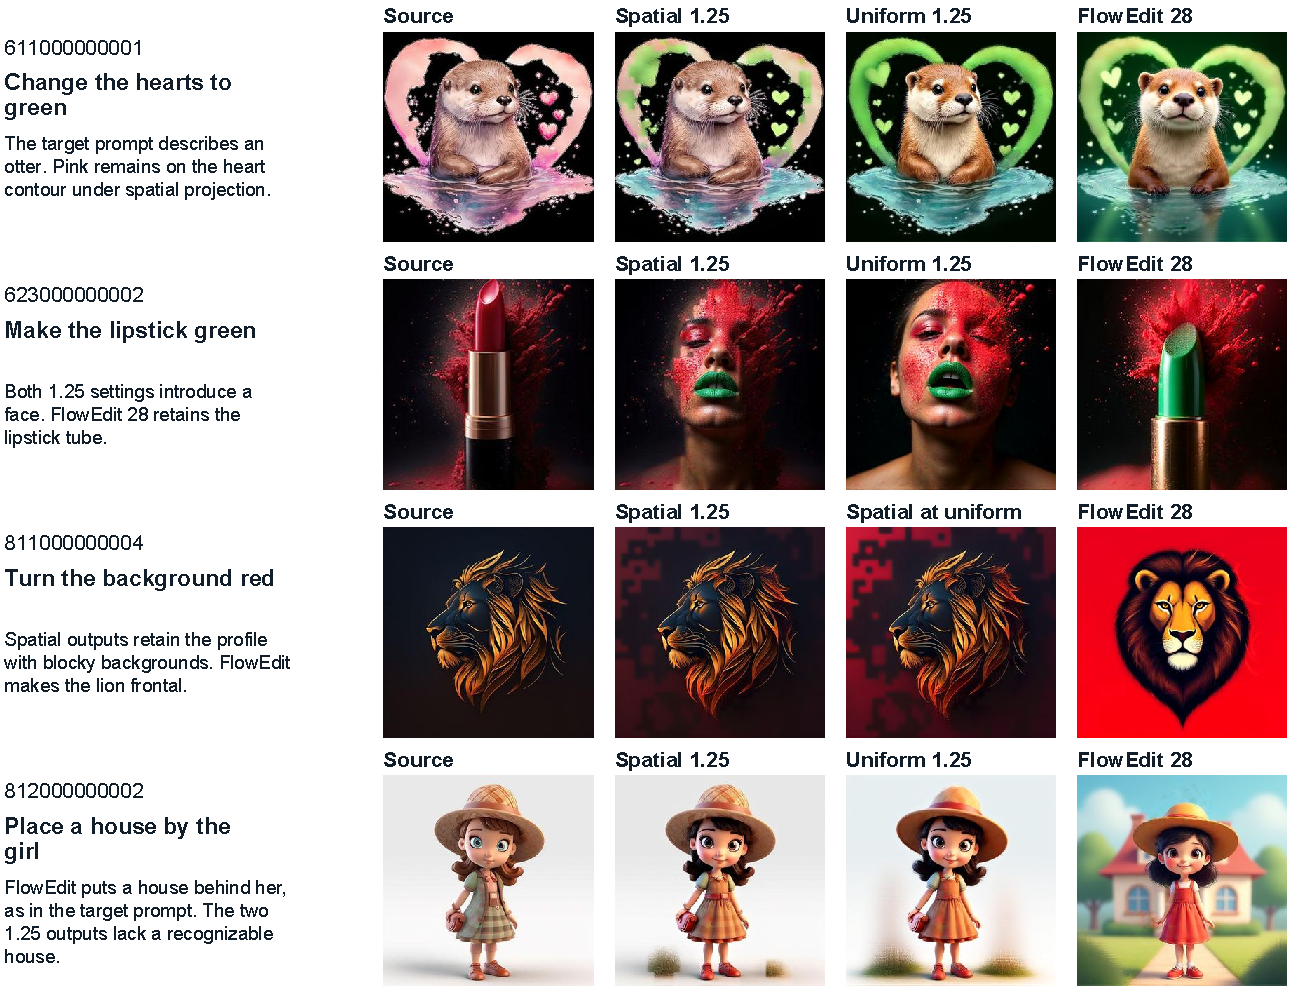
\includegraphics[width=.94\textwidth]{supp_cases_2.pdf}
\caption{Background, subject identity and prompt interpretation. The otter and house examples are the two observed raw-instruction/target-prompt discrepancies. The figure describes the supplied model target for each. The primary comparison includes both sources.}
\label{fig:sam-cases2}
\end{figure*}

\section{Post Hoc Checks on Recorded Trajectories and Outputs}
\label{sec:v21-checks}
\subsection{Native operating curves at the response attained by a control}
\label{sec:v21-points}
The two-constant and spatial-at-uniform runs each provide one measured output per source. For each of the 42 SAM sources with background pixels, we place that output at its measured directional CLIP on the same image's five-setting native curve. We interpolate background LPIPS in setting order only within the measured response range. The contrast is interpolated native loss minus observed point loss: a negative value favors the native sweep. This post hoc point comparison complements MRC, which averages over an interval.

\begin{table}[t]\centering\footnotesize
\caption{Native sweeps evaluated at the response attained by a measured control. Source support is pair-specific. Intervals use 10,000 paired-source bootstrap draws stratified by category among the supported sources. The final column repeats the mean with the last crossing.}
\label{tab:v21-points}
\setlength{\tabcolsep}{2pt}
\begin{tabular}{@{}llrll@{}}\toprule
Point & Sweep & $n$ & First crossing [95\% CI] & Last\\\midrule
Constants & Spatial & 36 & $-.0149\;[-.0374,.0193]$ & $-.0094$\\
Constants & Uniform & 36 & $+.0066\;[-.0063,.0201]$ & $+.0230$\\
Spatial/$U$ & Spatial & 32 & $-.0468\;[-.0936,-.0151]$ & $-.0311$\\
Spatial/$U$ & Uniform & 20 & $+.0008\;[-.0378,.0417]$ & $+.0071$\\\bottomrule
\end{tabular}
\end{table}

At the constants' response, the spatial sweep yields lower background loss on 35/36 supported sources (median difference $-0.0239$). One source contributes a difference of $+0.5542$. The first-crossing interval for the mean includes zero. The uniform sweep's mean changes from $+0.0066$ to $+0.0230$ with the crossing convention. These comparisons evaluate the single observed constant setting for each source. Its own response curve would require several gains per source. At the response of Spatial/$U$, the ordinary spatial sweep yields lower background loss on 24/32 sources. The replay estimates an allocation effect at the prescribed magnitude profile; the native sweep answers which measured settings preserve background at the replay's response.

\paragraph{Matching the spatial share of pixel change.} As a separate descriptive coordinate, we repeat the within-image integral with $\rho$, the fraction of absolute pixel change inside the edit region. Of 42 sources, 32 have positive-width spatial/uniform overlap in $\rho$ (median width 0.0437). The uniform-minus-spatial loss is $+0.0499$ [0.0271, 0.0746] on the first crossing and $+0.0834$ [0.0513, 0.1177] on the last; 29/32 differences are positive under each rule. These intervals resample supported sources with equal weight as in the original MRC analysis. Equal shares can accompany different total changes, different within-region patterns and different semantic outcomes.
\subsection{How closely can two constants fit the native projection profiles?}
\label{sec:v21-constants}
For each of 50 SAM sources, the native spatial run and its two-constant run record 26 aligned active steps at seed zero. Let $r^S_t$ and $r^C_t$ be the ungated source-relative displacement RMS on these two trajectories, and $b_{kt}$ the native projected RMS on branch $k$ (model or visible). The implemented gain is $g_k=\sum_t b_{kt}/\sum_t r^S_t$. Its relative summed magnitude on the constant trajectory is therefore $g_k\sum_t r^C_t/\sum_t b_{kt}=\sum_t r^C_t/\sum_t r^S_t$ for either branch, up to rounding. Both branches inherit the same mean signed overshoot of 8.42\%.

We held the measured $r^C_t$ fixed and fitted gains in $[0,1]$. For $d_t=g r^C_t-b_{kt}$, total error is $|\sum_t d_t|/\sum_t b_{kt}$ and step error is $\sum_t|d_t|/\sum_t b_{kt}$. Each active step enters once. One per-source fit matches the native sum exactly. A second minimizes step error using the weighted median of $b_{kt}/r^C_t$ with weights $r^C_t$. For the held-out comparison, we fit one gain per branch to minimize mean source step error on the other 49 sources and score the held-out source.

\begin{table}[t]
\centering\small
\caption{Absolute total and step errors on the recorded two-constant trajectories, as percentages of native branch magnitude, averaged over 50 sources. The first row uses measured FP32 projections.}
\label{tab:v21-constants}
\begin{tabular}{@{}lrrrr@{}}
\hline
 & \multicolumn{2}{c}{Model} & \multicolumn{2}{c}{Visible}\\
Gain & Total & Step & Total & Step\\
\hline
Executed per-source gain & 8.89 & 9.84 & 8.89 & 11.68\\
Per-source, match sum & 0.00 & 3.40 & 0.00 & 7.46\\
Per-source, minimum step error & 1.08 & 3.25 & 2.47 & 7.15\\
Shared, leave one source out & 9.60 & 10.26 & 15.77 & 18.04\\
\hline
\end{tabular}
\end{table}

Even at the best per-source gain, the visible profile has more step error than the model profile on 49/50 sources. The mean paired difference is 3.90 percentage points (95\% source-bootstrap interval 3.33--4.50; 10,000 draws, seed zero). The archived post-cast measurements give step errors of 9.83\% and 11.70\% for the executed model and visible branches. Changing a gain during generation would also change subsequent displacements. The three refitted rows quantify profile fit conditional on the recorded states; image-level effects would require new rollouts.

\subsection{Bounded-range SAM matched response}
\label{sec:v21-bounded}
The specified SAM sweep extends to scale 1.25. As a post hoc sensitivity analysis, we retain scales 0.25, 0.50, 0.75 and 1.00 on both arms, keeping their model and visible projection coefficients in $[0,1]$. Each source contributes its mean uniform-minus-spatial background LPIPS difference over the positive-width directional-CLIP overlap, using the first crossing in increasing scale order. The retained fraction divides this cohort mean by the mean scale-1 difference on exactly the same sources. Each of 10,000 paired source-bootstrap draws recomputes both means and their ratio.

\begin{table*}[t]
\centering\footnotesize
\caption{SAM matched-response estimates by scale range and background scorer. Positive differences favor spatial allocation. The common-source row evaluates the full grid on the 40 sources supported by the bounded grid. Brackets give percentile 95\% intervals.}
\label{tab:v21-bounded}
\setlength{\tabcolsep}{4pt}
\begin{tabular}{@{}llrrrrl@{}}
\hline
Background scorer & Range & Supported & $+/-$ & Default $U-S$ & Matched $U-S$ [95\% CI] & Retained [95\% CI]\\
\hline
Feature map & Full & 41/42 & 37/4 & 0.1207 & $0.0390\ [0.0106,0.0632]$ & 32.4\% [7.7\%, 57.4\%]\\
 & Bounded & 40/42 & 37/3 & 0.1233 & $0.0263\ [0.0169,0.0370]$ & 21.3\% [13.2\%, 30.5\%]\\
 & Full, common sources & 40/42 & 37/3 & 0.1233 & $0.0413\ [0.0121,0.0656]$ & 33.5\% [8.4\%, 58.9\%]\\
\hline
Masked input & Full & 41/42 & 37/4 & 0.0658 & $0.0326\ [0.0204,0.0462]$ & 49.4\% [34.5\%, 64.4\%]\\
 & Bounded & 40/42 & 36/4 & 0.0672 & $0.0179\ [0.0109,0.0262]$ & 26.7\% [18.5\%, 34.5\%]\\
 & Full, common sources & 40/42 & 37/3 & 0.0672 & $0.0345\ [0.0224,0.0479]$ & 51.4\% [37.1\%, 65.8\%]\\
\hline
\end{tabular}
\end{table*}

Removing scale 1.25 eliminates the jar's overlap and narrows the interval on 29 of the 40 remaining sources. On those 40 sources, the feature-map contrast changes by $-0.0150$ $[-0.0337,0.0098]$ and the retained fraction by $-12.2$ percentage points $[-31.3,6.7]$. Two source contrasts exchange signs. Restricting both grids to the same bounded response intervals recovers every bounded estimate: within those intervals, an earlier segment already reaches each response.

\subsection{Interpolation at held-out scan settings}
\label{sec:v21-grid}

We withheld each of the three interior settings in turn from each source and arm. Linear interpolation between the two neighboring knob settings predicts both coordinates of the held-out image. On 42 sources with a background (126 holdouts per arm), mean absolute directional-CLIP errors were 0.0257, 0.0237 and 0.0414 for spatial SAM (S), uniform SAM (U) and FlowEdit (F); background feature-map LPIPS errors were 0.0098, 0.0323 and 0.0592. A second test predicts LPIPS at the held image's \emph{observed} CLIP response, taking the first crossing of the four retained settings in knob order. The retained ranges covered 93, 95 and 92 of 126 queries, respectively. Mean absolute LPIPS errors on those queries were 0.0154, 0.0429 and 0.0593. Each source contributes its mean absolute error; the response-space test omits out-of-range queries. When the response folds, the first crossing may belong to a different branch from the held setting.

At seed 0, thinning the extended scan to scales 0.25, 0.75 and 1.25 preserved all 41 supported U$-$S sources and their signs. The mean first-crossing gap rose from 0.0390 on five scales to 0.0553 on three, a paired increase of 0.0163 [0.0070, 0.0271] (10,000 source-bootstrap draws). Both grids include the extrapolated 1.25 endpoint. The primary estimate of 0.0263 uses four scales up to 1.00 (Section~\ref{sec:v21-bounded}). The overlap narrowed on 23 sources. Integrating both grids over the three-point interval gave a similar increase, 0.0155 [0.0053, 0.0270]. F$-$S retained 38 sources with one sign change; F$-$U retained 40 of 41 with seven sign changes.

\begin{table}[t]
\centering\footnotesize
\caption{The four sources favoring uniform on the five-point grid. Width is the shared directional-CLIP range; $D$ is mean U$-$S background LPIPS on that range. The final column counts negative contrasts when both arms omit the same single interior rank.}
\label{tab:v21-grid-exceptions}
\setlength{\tabcolsep}{3pt}
\begin{tabular}{@{}lrrrrc@{}}
\hline
& \multicolumn{2}{c}{Five settings} & \multicolumn{2}{c}{Three settings} & Negative\\
Edit & Width & $D$ & Width & $D$ & deletions\\
\hline
Reflection & 0.03637 & $-0.0674$ & 0.03438 & $-0.0826$ & 3/3\\
Dog posture & 0.08516 & $-0.0119$ & 0.07049 & $-0.0072$ & 2/3\\
Jar lid & 0.00167 & $-0.0514$ & 0.00167 & $-0.0513$ & 3/3\\
Rice field & 0.04378 & $-0.3656$ & 0.04378 & $-0.2396$ & 3/3\\
\hline
\end{tabular}
\end{table}

Omitting scale 0.75 from both arms reverses the dog-posture contrast to $+0.0038$. The jar has the narrowest overlap of the 41 sources, $[0.02465,0.02632]$ directional CLIP. Its contrast stays between $-0.05171$ and $-0.05093$ across all nine joint or single-arm deletions. These checks measure interpolation at existing settings and sensitivity to thinning. A genuinely denser scan would require outputs at additional settings.

\noindent\textit{Thinning within the bounded range.}
With both endpoints fixed at 0.25 and 1.00, the four-setting U$-$S feature-map LPIPS contrast was 0.0263 on 40 supported sources. Keeping 0.50 as the sole interior setting gave 0.0330 on 38 sources. Keeping 0.75 gave 0.0292 on 39. Relative to the four-setting estimate on each subset's own sources, the paired increases were 0.0055 [0.0003, 0.0113] and 0.0023 [0.0003, 0.0039], respectively. On the 37 sources supported by all three grids, the four-setting grid and the two thinned grids retained 25.1\%, 30.1\% and 27.0\% of the same scale-1 default difference.

\subsection{Map placement, smoothness and correction energy}
\label{sec:v21-map}
Across 40 restoring sources, the native protection map ranked preservation pixels above edit pixels with mean AUROC 0.721. Rotating or reflecting each map on its square grid preserved its histogram and total variation (TV) exactly. Averaging the seven other orientations reduced AUROC to 0.550 (paired difference 0.171 [0.107, 0.231]). Conversely, shuffling cells with identical edit and preservation pixel counts preserved AUROC exactly while raising mean neighboring-cell variation from 0.076 to 0.188. An independent, prompt-free RGB center--surround contrast map gave edit-mask AUROC 0.575 [0.503, 0.642]. It measures local appearance contrast.

At the same initial state, archived pre-gain norms give the fraction of correction energy retained by a map, $q=\lVert P c_0\rVert_2^2/\lVert c_0\rVert_2^2$. Mean $q$ was 0.510 for the native map, 0.570 for cell permutation and 0.623 for histogram-matched reversal. The native-minus-permuted difference was $-0.060$ [$-0.080$, $-0.044$].

Across six archived map families at the native spatial RMS profile, a 0.10 higher AUROC was associated with a 0.00195 [0.00063, 0.00311] larger background-LPIPS gain over uniform, adjusting for source, map family and TV. Of 38 sources showing both wins and losses, 14 had a lower-AUROC map that beat uniform and a higher-AUROC map that lost. This ordering precludes a single AUROC cutoff for those sources. Intervals resample sources after averaging seeds 0 and 17.

\subsection{Does trajectory attenuation predict the preservation gap?}
\label{sec:v21-transfer}
We tested whether the relative magnitude of two unmodified rollouts adds predictive information beyond the background area fraction. For each source the target was $G=L_U-L_S$, the uniform minus spatial background LPIPS. Positive $G$ favors spatial allocation for both restoring and departing operators. The primary score averages the AlexNet LPIPS feature map over the same annotated background used to measure area. The additional predictor was $a=1-I_S/I_U$. For restoring correction, $I$ sums applied velocity RMS weighted by the integration step. For DirectEdit, $I$ sums the actual blend-displacement RMS, which is already in latent displacement units. For SAM, the ratio uses the mean visible-branch displacement RMS over 26 active steps. Each ratio compares the two realized trajectories of one editor.

\paragraph{Transfer between restoring operators.}
Twenty DirectEdit sources have the same decoded source pixels, annotation masks and prompt pairs as 20 of the 40 correction sources. We fit ordinary least squares on the other 20 correction sources, using generation seed 0. We applied the frozen coefficients to the held-out 20 sources in both editors. Both comparisons use unmodified spatial and uniform arms at coefficient 0.25. In DirectEdit these are the local and global blend controls. The reference mask also enters the DirectEdit blend, whereas the correction editor constructs its own weight map. The training attenuation range was $[0.184,0.319]$. On the same test images all 20 correction ratios were in range, while 17 DirectEdit ratios fell outside it ($[-0.635,0.713]$). In ten DirectEdit cases the spatial trajectory had greater cumulative magnitude than the uniform one, giving negative attenuation.

\begin{table}[t]\centering
\caption{Held-out RMSE for predicting $G$. The last column gives the paired error reduction from adding attenuation and its 95\% bootstrap interval. The first three rows use feature-map LPIPS.}
\label{tab:v21-transfer}
{\footnotesize\setlength{\tabcolsep}{1.5pt}
\begin{tabular*}{\columnwidth}{@{\extracolsep{\fill}}lrrl@{}}\toprule
Test set & Area & Area $+a$ & Gain [95\% interval]\\\midrule
Correction & 0.0296 & 0.0295 & $0.00002\;[-0.00063,0.00088]$\\
DirectEdit & 0.0340 & 0.0332 & $0.00085\;[-0.01749,0.00341]$\\
SAM, category & 0.1138 & 0.1039 & $0.00988\;[-0.00156,0.02328]$\\
SAM, masked input & 0.0501 & 0.0464 & $0.00373\;[-0.00404,0.01328]$\\\bottomrule
\end{tabular*}}
\end{table}
The DirectEdit MAE reduction was 0.00116 [$-0.01467,0.00405$]. For the two operator rows, 5,000 bootstrap draws resampled training and test sources independently within edit category, refit both models, and used the same test draws for both operators. The small point gain, its interval and the feature-range shift leave the incremental predictive value on another operator unresolved.

\paragraph{Held-out edit categories in SAM.}
The departing operator used a disjoint cohort. We held out each entire PIE edit category in turn and fit the same models to the other nine. The 42 sources with a background enter the pooled error once each (one to five test sources per category). Area plus attenuation reduced feature-map MAE from 0.07954 to 0.07263, with a paired reduction of 0.00691 [$-0.00430,0.01873$]. Seven of ten categories had lower MAE. The intervals for SAM resample whole categories and refit each fold, keeping every copy of the test category out of training. With the original masked-input scorer, leave-one-source-out RMSE was 0.05011 versus 0.04630. Holding out the whole category gave 0.05013 versus 0.04639 on that same scorer. The two scorer scales are reported separately.

\paragraph{Prediction scope.}
The background fraction uses an evaluation annotation, and $a$ requires both test-image rollouts. This post hoc check concerns prediction after the two traces have been observed. The local archive contains three nested SAM report snapshots (245, 300 and 900 completed jobs), all on FLUX.1-dev at generation seed 0. The additional correction seeds belong to the restoring editor. The audited runs provide one transfer between two restoring operations on FLUX and a within-SAM category check. Transfer to a departing operator, another SAM generation seed or a second backbone remains unverified.


\section{Source Correction: Crossed Profiles and Cohort}
\subsection{Selection before generation}
The selection manifest excludes 90 historical source IDs and content duplicates. Eligible sources have valid prompts and nonempty official edited and preserved regions. Within each eligible category, selection follows a deterministic SHA256 ordering with the fixed study salt. Four sources are allocated to each category 0--8; four remaining slots go to categories 0--3. The resulting mixture has five sources in each of categories 0--3 and four in each of 4--8. After historical exclusions, remaining category-9 style cases lack a nonempty official preservation region and are outside this cohort.

Content deduplication uses an RGB exact hash or a perceptual dHash distance at most 8 combined with $64\times64$ thumbnail RGB MAE at most 12. This rule applies against historical and already selected images. The manifest records selected and excluded sources. ID disjointness and plan consistency are verified from these records; content deduplication requires the original historical images. Table~\ref{tab:r88-source-manifest40} lists all selected sources and original instructions.

The estimand weights each source equally in the planned 40-source mixture, so category weights follow the stated counts. Its population is the eligible selected cohort. All sources receive seeds 0 and 17, and every source/seed receives every arm. The archived design and statistical files specify these choices in internal frozen protocol artifacts; no public preregistration was recorded.

% Generated only from the archived R88 statistics and manifest; no tests rerun.
% Preamble dependencies: \usepackage{booktabs,tabularx,array}
% Natural 8 pt text in a 6.9 in-wide table; no resizebox scaling.
\begin{table*}[!t]
\centering
\begin{minipage}{6.9in}
\fontsize{8}{9.2}\selectfont
\caption{The fixed 40-source R88 cohort and original editing instructions.}
\label{tab:r88-source-manifest40}
\setlength{\tabcolsep}{3pt}
\renewcommand{\arraystretch}{1.08}
\begin{tabularx}{\linewidth}{@{}c l >{\raggedright\arraybackslash}X@{}}
\toprule
Category & Source ID & Original editing instruction \\
\midrule
0 & \texttt{000000000001} & Change the cake shape to square \\
0 & \texttt{000000000009} & Change the animal from a dog to a lion \\
0 & \texttt{000000000094} & Turn the color of the blanket from red to blue \\
0 & \texttt{000000000115} & Change the ducks to birds \\
0 & \texttt{000000000117} & Change the flower's color from pink to blue and the center from yellow to red \\
\addlinespace[1pt]
1 & \texttt{111000000000} & change the fishes to sharks \\
1 & \texttt{111000000003} & Change the bunny to a pig \\
1 & \texttt{112000000005} & Change the light source to the moon \\
1 & \texttt{113000000007} & Change the plant to a flower \\
1 & \texttt{122000000001} & change the spider man to robot \\
\addlinespace[1pt]
2 & \texttt{213000000001} & Add a pen to the table \\
2 & \texttt{214000000001} & Add deer in the forest \\
2 & \texttt{223000000006} & Add glasses to the desk \\
2 & \texttt{224000000006} & Add a surfer and sharks to the beach \\
2 & \texttt{224000000009} & Add a goat eating grass to the scene \\
\addlinespace[1pt]
3 & \texttt{312000000003} & Remove the bat from the scene \\
3 & \texttt{313000000001} & Remove the bulb \\
3 & \texttt{313000000006} & Remove the chair \\
3 & \texttt{322000000000} & Remove the cell phone \\
3 & \texttt{323000000008} & Remove the leaf design from the top of the coffee cups \\
\addlinespace[1pt]
4 & \texttt{414000000004} & Change the size of the mushrooms in the painting from huge to small \\
4 & \texttt{422000000002} & Change the woman's gaze to be looking forward \\
4 & \texttt{424000000000} & Change dimly illuminated to sunlit illuminated \\
4 & \texttt{424000000002} & Change the color of the car from white to stripe \\
\addlinespace[1pt]
5 & \texttt{512000000000} & Change the position of the woman's arms from up to down \\
5 & \texttt{513000000000} & Change the position of the chair to face backwards \\
5 & \texttt{521000000003} & Make the fox's head down \\
5 & \texttt{522000000002} & make the boy's hands up \\
\addlinespace[1pt]
6 & \texttt{612000000002} & make the circle cyan \\
6 & \texttt{613000000000} & Change the color of the flowers to blue \\
6 & \texttt{613000000001} & Change the color of the curtain from red to yellow \\
6 & \texttt{624000000002} & Change the sky's color to gray \\
\addlinespace[1pt]
7 & \texttt{711000000002} & Make the butterfly plastic \\
7 & \texttt{712000000002} & Change the woman to a golden sculpture \\
7 & \texttt{713000000000} & Make the chairs plastic \\
7 & \texttt{713000000004} & Change the cabinets to be wooden \\
\addlinespace[1pt]
8 & \texttt{811000000003} & Add a blue background to the digital painting \\
8 & \texttt{814000000004} & Change the painting from planets and stars to cats and dogs \\
8 & \texttt{822000000005} & Substitute the mountain with a garden \\
8 & \texttt{822000000006} & Change trees to elves \\
\bottomrule
\end{tabularx}
\par\smallskip
{\raggedright Source IDs preserve all leading zeros. Instructions are copied verbatim from the official records and match the executed task edit rubrics; capitalization and wording are retained. Categories: 0: random editing; 1: change object; 2: add object; 3: delete object; 4: change attribute content; 5: change attribute pose; 6: change attribute color; 7: change attribute material; 8: change background. Categories 0--3 contribute five sources each and 4--8 four each; category 9 is absent under the fixed nonempty-preservation eligibility rule. Every source has seeds 0 and 17 and all six arms (480 outputs). These instructions describe the intended edit; they are not outcome judgments. The model conditioning used the archived source/target prompts, while wrong-target probes retained the original edit target.\par}
\end{minipage}
\end{table*}


\subsection{Notation}
Table~\ref{tab:notation} summarizes the main-paper symbols.
An \emph{allocation rule} specifies spatial weighting; its normalized residual is the \emph{correction direction}. A \emph{magnitude profile} (also called dose profile in historical records) is the full stepwise applied RMS sequence. Its step-size-weighted sum is the \emph{cumulative correction magnitude} $I$. These quantities measure the source-correction term, separately from the target field, the complete update, and semantic editing strength. RMS and its cumulative sum are norm quantities; squared residuals enter the separate attenuation identity below. The \emph{uniform} rule is called \emph{global} in historical arm names and records (e.g., GLB-R). \emph{Request-weighted} denotes the map construction, whereas REQ names its native arm. Native comparisons share a coefficient; matched-RMS comparisons share an applied sequence.
\begin{table}[!t]
\centering\small
\caption{Main-paper symbols. Spatial weights are broadcast over channels.}
\label{tab:notation}
\begin{tabularx}{\linewidth}{@{}l >{\raggedright\arraybackslash}X@{}}
\toprule
Symbol & Meaning\\
\midrule
$z_i,r_i$ & Edited state and reference state at step $i$\\
$\sigma_i,h_i$ & Decreasing scheduler node; $h_i=\sigma_i-\sigma_{i+1}$\\
$u_i^s,u_i^{t,M_{\rm KV}}$ & Source field and target field with fixed source memory $M_{\rm KV}$\\
$c_i,\widehat c_i$ & Current-state residual and applied correction\\
$E,P$ & Normalized prompt response and protection weight $P=1-0.75E$\\
$e_i(P)$ & Same-state residual-energy-weighted mean of $P^2$\\
$\lambda$ & Native correction coefficient, 0.25\\
$b_i^R,b_i^U$ & RMS profiles recorded by native REQ and U25\\
$I$ & Cumulative magnitude $\sum_i h_i\RMS(\widehat c_i)$\\
$\beta$ & Multiplier on the uniform-origin profile\\
$\gamma$ & Controlled-inversion mixture, 0.5\\
\bottomrule
\end{tabularx}
\end{table}

\subsection{Fixed editor and probe settings}
The backbone is FLUX.1-dev with $512\times512$ images, 28 integration steps, guidance 3.5, inversion mixture $\gamma=0.5$, network evaluation in BF16, and integration in FP32. Source K/V memory is paired with reference states, read by all image queries, and injected at steps 0--6 in single-stream blocks 1--26. Gate strength is one in all six arms. These are fixed development choices, not settings selected on the new outputs.

The native correction coefficient is $\lambda=0.25$. At reference states nearest scheduler values $0.25,0.50,0.75$, channel-RMS source/target velocity differences yield response maps. Each map is normalized by its 10th and 90th spatial percentiles and clipped to $[0,1]$; a degenerate range contributes zero. Averaging the three maps gives $E$, and protection weights are $P=1-0.75E$. Thus $P\in[0.25,1]$: response-high locations receive weaker source correction. Official masks enter evaluation and cohort eligibility, not this map construction.

\paragraph{Reference trajectory and fields.}
With a seed-fixed Gaussian endpoint $\epsilon$, controlled inversion uses increasing times $t_k$ and Euler updates
\begin{equation}
z_{k+1}=z_k+\Delta t_k\left[(1-\gamma)f_\theta(z_k,t_k;\emptyset,0)
+\gamma\frac{\epsilon-z_k}{1-t_k}\right].
\end{equation}
The second term points toward the Gaussian endpoint; reversing the saved states supplies the generation reference. The last argument of $f_\theta$ is guidance strength. During editing, $u_i^s(z_i)=-f_\theta(z_i,\sigma_i;c_s,3.5)$ is evaluated with memory disabled. The target field uses the same sign convention, target prompt, and fixed K/V rule. Together with the own-state update in main-paper Eq.~(5), these definitions specify the reference displacement and current-state residual; editing-controller parameters are $\eta=0$ and $\tau=1$.

\paragraph{Budget-preserving K/V rule.}
For each image query/head, native joint attention is $a=\mathrm{softmax}(q[K_T,K_I]^\top/\sqrt d)$, with text and image keys $K_T,K_I$ and head width $d$. Let $m_I=\sum_{j\in I}a_j$. The memory output is
\begin{equation}
\widetilde o=a_TV_T+m_I\,\mathrm{softmax}(qK_S^\top/\sqrt d)V_S.
\end{equation}
Source keys/values $K_S,V_S$ are captured by a source-prompt forward pass at reference state $r_i$. The rule retains the native text contribution and image-attention mass while reallocating that mass to source values. Steps 0--6 and blocks 1--26 are inclusive, zero-based indices. The six-arm comparison uses gate one for every image query in these blocks; other operations retain native attention.

\subsection{Six interventions}
Let $c_i$ be the correction evaluated at an arm's own edited state and let $b_i^R$ and $b_i^U$ be the actual RMS profiles recorded by native request and uniform runs. The interventions are:
\begin{align}
\mathrm{REQ}:&\quad \widehat c_i=0.25P\odot c_i,\\
\text{GLB-R}:&\quad \widehat c_i=b_i^R c_i/\RMS(c_i),\\
\mathrm{U25}:&\quad \widehat c_i=0.25c_i,\\
\text{REQ-U}:&\quad \widehat c_i=b_i^U(P\odot c_i)/\RMS(P\odot c_i).
\end{align}
In semantic terms, REQ is Spatial@spatial-profile, GLB-R is Uniform@spatial-profile, U25 is Uniform@uniform-profile, and REQ-U is Spatial@uniform-profile. The native arms record the two profiles; the crossed arms replay them. Historical identifiers remain in tables and filenames to connect each comparison to its archived records.

SHUF-R and REV-R use the same normalization as REQ-U, but target $b_i^R$ and replace $P$ with the corresponding control map. A zero direction with a positive target norm is infeasible and is treated as an execution error, not silently replaced. The six-arm replay implementation rejects nonpositive targets; the subsequent eight-arm extension also handles a zero target by applying zero correction. Every recorded anchor is positive (minimum RMS 0.08143), so the implemented positive-target domain covers all reported runs.

For SHUF-R, a fixed cyclic derangement chooses another target prompt within the same category. The donor ordering and smallest shift giving distinct target prompts are fixed before generation. Probes use the \emph{recipient} image, source prompt, and reference states with the wrong target. Their resulting weights are rank matched to the correct map's sorted values. The generation prompt remains the recipient's original correct target. This changes the target used to form the map, not the requested edit being generated. Rank matching preserves the weight histogram, not all spatial morphology.

REV-R uses $P^{\mathrm{rev}}=1.25-P$, preserving the range $[0.25,1]$ while reversing spatial emphasis. Its histogram generally changes. This differs from the prior block-permutation control, which rearranged blocks of an already computed map. Figure~\ref{fig:maps} shows actual correct, wrong-request, and reversed maps.

\begin{figure*}[!t]
\centering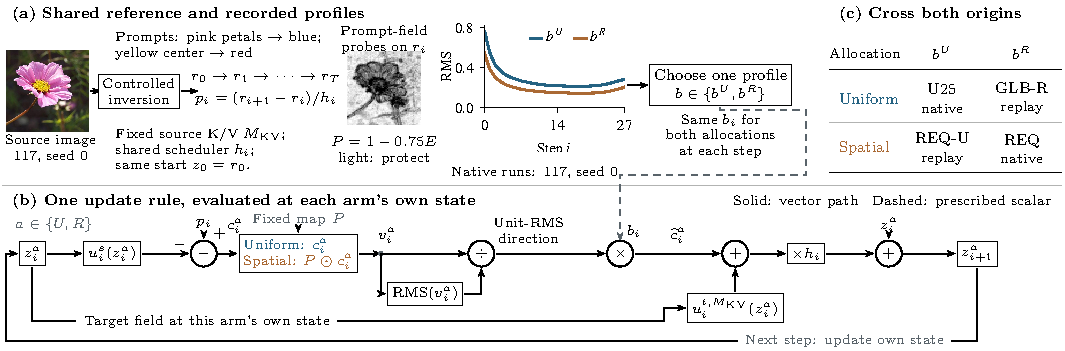
\includegraphics[width=\textwidth]{figures/method_diagram_v14.pdf}
\caption{Detailed crossed-profile protocol retained from the earlier main-paper diagram. The source image, protection map, and two native 28-step RMS curves use source 000000000117, seed 0. Native runs share the reference and record request- and uniform-origin profiles; each replay arm recomputes its residual and target field at its own evolving state. Crossing allocation with profile origin forms the four comparison cells. The flow diagram specifies the computation; its arrows are not measured latent trajectories.}
\label{fig:protocol-flow}
\end{figure*}

\begin{figure*}[!t]
\centering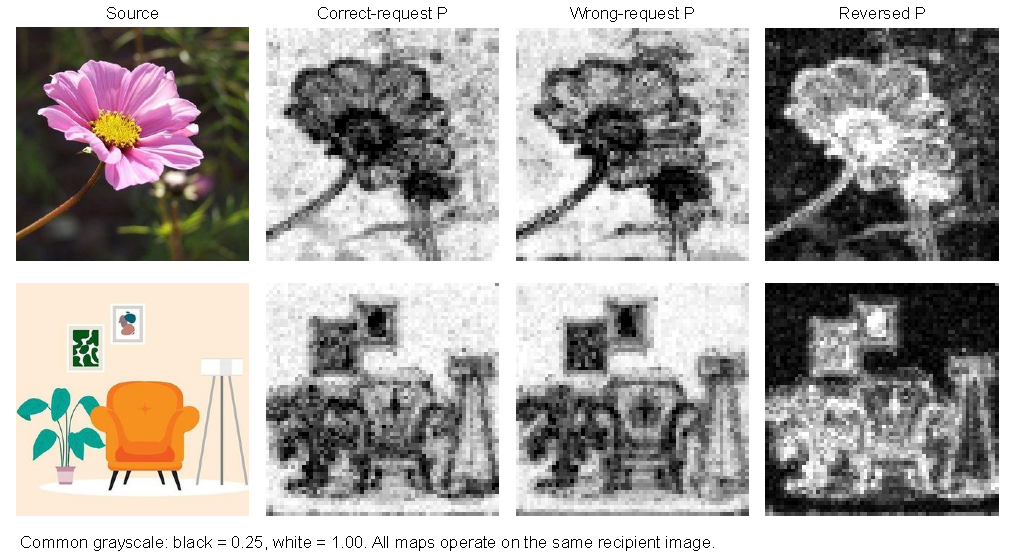
\includegraphics[width=\textwidth]{figures/maps.pdf}
\caption{Actual maps for two fresh-source examples. Each row shows the source and the correct-request, wrong-request, and reversed protection weights. Higher values apply stronger source correction. The wrong-request map is computed on the same source with a fixed donor target, then histogram matched; reversal retains the allowed value range. Maps visualize weighting, not ground-truth edit localization.}
\label{fig:maps}
\end{figure*}

\section{Allocation Effects at Matched Profiles}
The four crossed cells separate two uses of an ablation. REQ versus U25 compares native configurations, including the profiles they induce. REQ versus GLB-R and REQ-U versus U25 compare spatial allocation at the request- and uniform-origin profiles, respectively. Reporting their joint outcomes makes the conditional preservation effect visible alongside editing response.
\begin{table*}[!t]
\centering\small
\caption{Six-arm cohort means after seed averaging within 40 sources. Arrows indicate preferred metric direction. Profile groups follow the main-paper factorial comparison.}
\label{tab:main-means}
\begin{tabular}{lrrrrrr}
\toprule
Arm & Target CLIP $\uparrow$ & Dir. CLIP $\uparrow$ & DINOv2 $\uparrow$ & Full LPIPS $\downarrow$ & Pres. LPIPS $\downarrow$ & Pres. MAE $\downarrow$\\
\midrule
REQ &0.2643&0.1288&0.5406&0.5449&0.5254&0.1239\\
GLB-R &0.2647&0.1297&0.5396&0.5528&0.5353&0.1266\\
U25 &0.2665&0.1357&0.5545&0.5045&0.4891&0.1051\\
REQ-U &0.2647&0.1291&0.5540&0.4974&0.4791&0.1023\\
SHUF-R &0.2648&0.1300&0.5388&0.5452&0.5265&0.1251\\
REV-R &0.2673&0.1344&0.5349&0.5719&0.5575&0.1388\\
\bottomrule
\end{tabular}
\end{table*}
\subsection{Pairing, outcomes, and uncertainty}
For each metric and arm, the two seed values are averaged within source. Contrasts then use 40 independent source-level differences. Retaining all arms of a source together preserves pairing. The primary metric is preservation LPIPS, computed by averaging a spatial LPIPS map over the official preservation mask. LPIPS receptive fields can extend across the mask boundary. Full-image LPIPS, preservation RGB MAE on $[0,1]$ channels, full-image DINOv2 cosine similarity, target CLIP, and directional CLIP complete the six-metric family. Scores were evaluated on native server PNGs. JPEG previews in the compact archive support figures rather than metric recomputation.

\paragraph{Image inputs and evaluators.}
Source and native output images are converted to RGB and resized to $512\times512$ with Lanczos. LPIPS uses AlexNet v0.1 with ImageNet trunk and learned calibration weights loaded explicitly, both with strict state-dictionary checks. Inputs are mapped to $[-1,1]$. Full LPIPS averages feature distances over the complete image; spatial LPIPS is also evaluated on complete images, then weighted by preservation mask $W$. If needed, $W$ is resized to the feature-distance map with area interpolation. Images are neither cropped nor zero-masked before feature extraction.

CLIP uses OpenAI ViT-L/14 and image-feature similarity uses DINOv2-base. After the RGB/$512\times512$ input step, each evaluator calls its local checkpoint processor. DINO compares the first token of \texttt{last\_hidden\_state} by cosine. Target CLIP is an image--text cosine. For directional CLIP, writing $N(v)=v/\|v\|_2$, the implemented score is
\begin{equation}
\cos\!\left(N(I_{\rm edit})-N(I_{\rm src}),\,
N(T_{\rm target})-N(T_{\rm src})\right).
\end{equation}
A zero difference is recorded as missing. Scores are raw cosines without logit scaling or positive clipping. 

\paragraph{Evaluation-mask convention.}
The decoder maps zero-based RLE start/length pairs to a row-major $512\times512$ edit mask $M_{\rm edit}$, then marks the first/last rows and columns as edited. This excludes the one-pixel image frame from $W=1-M_{\rm edit}$; it does not dilate the annotated object boundary. RGB MAE weights pixels by $W$ for preservation and by $M_{\rm edit}$ for edit-region change. Spatial LPIPS similarly weights its output map, whose receptive fields still include adjacent pixels. The native audit below reports the original, official, and 8-/16-pixel interior masks (Table~\ref{tab:r89-native-boundary}).

Confidence intervals use 20,000 paired category-stratified source bootstraps with PCG64 and base seed 88002. Every replicate retains the planned category counts. Percentile bounds are the 2.5th and 97.5th percentiles with linear interpolation. The same resampled source weights are used across metrics and decomposition components for a cohort. Intervals are marginal; the separately reported adjusted tests address multiplicity.

Two-sided sign-flip tests use $B=1,000,000$ Monte Carlo sign assignments, base seed 88001, and the absolute mean source difference. The same assignments are used for all contrasts and outcomes. With $k$ assignments at least as extreme as the observation (tolerance $10^{-12}$),
\begin{equation}
p_{\mathrm{MC}}=(k+1)/(B+1).
\end{equation}
This is Monte Carlo inference, not exhaustive enumeration of $2^{40}$ assignments. It assumes independent source differences with a sign-invariant joint distribution under the null; a zero mean alone does not imply that condition. The primary comparison has $k=267$, $p=0.0002679997$, and approximate Monte Carlo standard error $1.64\times10^{-5}$. Zero-extreme contrasts have the resolution floor $1/(B+1)$, not $p=0$.

\subsection{Primary, secondary, and sensitivity families}
The primary test is REQ-U minus U25 preservation LPIPS, two-sided $\alpha=0.05$. On passing this gate, four secondary preservation tests use Holm correction: REQ minus GLB-R, direction-by-profile interaction, REQ minus SHUF-R, and REQ minus REV-R. Reported gated values are the maximum of primary $p$ and secondary Holm4 $p$. The primary effect is negative and the gate opens. The sensitivity family comprises these five contrasts crossed with all six outcomes: Holm30. It supplements rather than replaces the specified primary test.

Table~\ref{tab:r88-paired-all30} supplies every contrast. Seven of 30 tests pass Holm30: the three preservation contrasts against U25, GLB-R, and REV-R; full LPIPS against GLB-R and REV-R; and preservation MAE against SHUF-R and REV-R. All CLIP and DINO tests and every interaction test remain above 0.05 under that family. Some marginal intervals exclude zero despite a nonsignificant Holm30 value because intervals and adjusted tests use different coverage criteria.

% Generated only from the archived R88 statistics and manifest; no tests rerun.
% Preamble dependencies: \usepackage{booktabs,tabularx,array}
% Natural 8 pt text in a 6.9 in-wide table; no resizebox scaling.
\begin{table*}[!t]
\centering
\begin{minipage}{6.9in}
\fontsize{8}{9.2}\selectfont
\caption{All planned contrasts: five comparisons across six outcomes.}
\label{tab:r88-paired-all30}
\setlength{\tabcolsep}{3pt}
\renewcommand{\arraystretch}{1.05}
\begin{tabularx}{\linewidth}{@{}l r >{\centering\arraybackslash}X r r r@{}}
\toprule
Metric & $\Delta$ & Pointwise 95\% CI & $p_{\rm raw}$ & $p_{\rm gate}$ & $p_{\rm Holm30}$ \\
\midrule
\multicolumn{6}{@{}l}{\textbf{$\mathrm{REQ\_U}-\mathrm{U25}$; primary contrast}} \\
LPIPS preserved $\downarrow$ & $-0.01003$ & $[-0.01531,\,-0.00511]$ & $2.680\times 10^{-4}$ & $2.680\times 10^{-4}$ & $0.006700$ \\
CLIP target $\uparrow$ & $-0.00179$ & $[-0.00401,\,0.00037]$ & $0.217472$ & \textemdash & $1$ \\
CLIP directional $\uparrow$ & $-0.00658$ & $[-0.01438,\,0.00048]$ & $0.140665$ & \textemdash & $1$ \\
DINO full $\uparrow$ & $-0.00055$ & $[-0.00803,\,0.00680]$ & $0.908618$ & \textemdash & $1$ \\
LPIPS full $\downarrow$ & $-0.00712$ & $[-0.01242,\,-0.00226]$ & $0.018093$ & \textemdash & $0.385528$ \\
Preserved MAE $\downarrow$ & $-0.00282$ & $[-0.00467,\,-0.00086]$ & $0.017524$ & \textemdash & $0.385528$ \\
\midrule
\multicolumn{6}{@{}l}{\textbf{$\mathrm{REQ}-\mathrm{GLB\_R}$; secondary preservation contrast}} \\
LPIPS preserved $\downarrow$ & $-0.00996$ & $[-0.01389,\,-0.00639]$ & $6.000\times 10^{-6}$ & $2.680\times 10^{-4}$ & $1.620\times 10^{-4}$ \\
CLIP target $\uparrow$ & $-0.00030$ & $[-0.00199,\,0.00139]$ & $0.771000$ & \textemdash & $1$ \\
CLIP directional $\uparrow$ & $-0.00093$ & $[-0.00639,\,0.00472]$ & $0.768916$ & \textemdash & $1$ \\
DINO full $\uparrow$ & $0.00096$ & $[-0.00662,\,0.00846]$ & $0.818317$ & \textemdash & $1$ \\
LPIPS full $\downarrow$ & $-0.00783$ & $[-0.01150,\,-0.00445]$ & $3.700\times 10^{-5}$ & \textemdash & $9.620\times 10^{-4}$ \\
Preserved MAE $\downarrow$ & $-0.00263$ & $[-0.00423,\,-0.00091]$ & $0.012488$ & \textemdash & $0.287224$ \\
\midrule
\multicolumn{6}{@{}l}{\textbf{$(\mathrm{REQ\_U}-\mathrm{U25})-(\mathrm{REQ}-\mathrm{GLB\_R})$; cross-anchor interaction}} \\
LPIPS preserved $\downarrow$ & $-0.00007$ & $[-0.00376,\,0.00372]$ & $0.975679$ & $0.975679$ & $1$ \\
CLIP target $\uparrow$ & $-0.00149$ & $[-0.00409,\,0.00107]$ & $0.393190$ & \textemdash & $1$ \\
CLIP directional $\uparrow$ & $-0.00566$ & $[-0.01484,\,0.00272]$ & $0.264773$ & \textemdash & $1$ \\
DINO full $\uparrow$ & $-0.00151$ & $[-0.01110,\,0.00783]$ & $0.802496$ & \textemdash & $1$ \\
LPIPS full $\downarrow$ & $0.00071$ & $[-0.00222,\,0.00361]$ & $0.707248$ & \textemdash & $1$ \\
Preserved MAE $\downarrow$ & $-0.00018$ & $[-0.00063,\,0.00023]$ & $0.467443$ & \textemdash & $1$ \\
\midrule
\multicolumn{6}{@{}l}{\textbf{$\mathrm{REQ}-\mathrm{SHUF\_R}$; secondary preservation contrast}} \\
LPIPS preserved $\downarrow$ & $-0.00116$ & $[-0.00269,\,0.00043]$ & $0.239479$ & $0.478958$ & $1$ \\
CLIP target $\uparrow$ & $-0.00045$ & $[-0.00173,\,0.00082]$ & $0.558413$ & \textemdash & $1$ \\
CLIP directional $\uparrow$ & $-0.00115$ & $[-0.00541,\,0.00299]$ & $0.629484$ & \textemdash & $1$ \\
DINO full $\uparrow$ & $0.00180$ & $[-0.00385,\,0.00748]$ & $0.578875$ & \textemdash & $1$ \\
LPIPS full $\downarrow$ & $-0.00028$ & $[-0.00140,\,0.00086]$ & $0.684543$ & \textemdash & $1$ \\
Preserved MAE $\downarrow$ & $-0.00113$ & $[-0.00187,\,-0.00050]$ & $0.001074$ & \textemdash & $0.025776$ \\
\midrule
\multicolumn{6}{@{}l}{\textbf{$\mathrm{REQ}-\mathrm{REV\_R}$; secondary preservation contrast}} \\
LPIPS preserved $\downarrow$ & $-0.03214$ & $[-0.04184,\,-0.02316]$ & $1.000\times 10^{-6}$ & $2.680\times 10^{-4}$ & $3.000\times 10^{-5}$ \\
CLIP target $\uparrow$ & $-0.00296$ & $[-0.00627,\,0.00004]$ & $0.113685$ & \textemdash & $1$ \\
CLIP directional $\uparrow$ & $-0.00561$ & $[-0.01613,\,0.00387]$ & $0.339445$ & \textemdash & $1$ \\
DINO full $\uparrow$ & $0.00566$ & $[-0.00485,\,0.01657]$ & $0.349881$ & \textemdash & $1$ \\
LPIPS full $\downarrow$ & $-0.02697$ & $[-0.03599,\,-0.01886]$ & $1.000\times 10^{-6}$ & \textemdash & $3.000\times 10^{-5}$ \\
Preserved MAE $\downarrow$ & $-0.01488$ & $[-0.01948,\,-0.01025]$ & $3.000\times 10^{-6}$ & \textemdash & $8.400\times 10^{-5}$ \\
\bottomrule
\end{tabularx}
\par\smallskip
{\raggedright Signed differences use 40 sources after averaging seeds 0 and 17. Intervals are marginal, category-stratified paired bootstrap intervals. The primary preservation test opens the four-test secondary gate; a dash marks outcomes outside it. Holm30 adjusts all rows. Monte Carlo values near $10^{-6}$ reflect the $1/1{,}000{,}001$ resolution floor. Arrows denote preferred metric direction. All effects use raw metric units.\par}
\end{minipage}
\end{table*}


\subsection{Distribution across sources}
For REQ-U minus U25 preservation LPIPS, 31 sources improve, nine worsen, and none tie. The median difference is $-0.006038$. Improvements of at least 0.005, 0.010, and 0.020 occur in 22, 14, and seven sources, respectively. These cutoffs describe numerical LPIPS differences; their perceptual interpretation would require independent observer calibration. REQ improves over GLB-R on 33/40 sources, over SHUF-R on 25/40, and over REV-R on 37/40. Table~\ref{tab:r88-source-wins} reports the planned thresholds for both anchor comparisons across all metrics. Thresholds use raw score units and have no human perceptual calibration.

% Generated only from the archived R88 statistics and manifest; no tests rerun.
% Preamble dependencies: \usepackage{booktabs,tabularx,array}
% Natural 8 pt text in a 6.9 in-wide table; no resizebox scaling.
\begin{table*}[!t]
\centering
\begin{minipage}{6.9in}
\fontsize{8}{9.2}\selectfont
\caption{Source-level metric improvements at every planned threshold.}
\label{tab:r88-source-wins}
\setlength{\tabcolsep}{3pt}
\renewcommand{\arraystretch}{1.08}
\begin{tabularx}{\linewidth}{@{}l *{4}{>{\centering\arraybackslash}X} c@{}}
\toprule
Metric & $g>0$ & $g\geq0.005$ & $g\geq0.010$ & $g\geq0.020$ & Ties \\
\midrule
\multicolumn{6}{@{}l}{\textbf{$\mathrm{REQ\_U}-\mathrm{U25}$}} \\
LPIPS preserved $\downarrow$ & 31 (77.5\%) & 22 (55.0\%) & 14 (35.0\%) & 7 (17.5\%) & 0 \\
CLIP target $\uparrow$ & 14 (35.0\%) & 7 (17.5\%) & 5 (12.5\%) & 1 (2.5\%) & 0 \\
CLIP directional $\uparrow$ & 16 (40.0\%) & 13 (32.5\%) & 9 (22.5\%) & 6 (15.0\%) & 0 \\
DINO full $\uparrow$ & 21 (52.5\%) & 18 (45.0\%) & 14 (35.0\%) & 8 (20.0\%) & 0 \\
LPIPS full $\downarrow$ & 26 (65.0\%) & 17 (42.5\%) & 11 (27.5\%) & 7 (17.5\%) & 0 \\
Preserved MAE $\downarrow$ & 30 (75.0\%) & 15 (37.5\%) & 6 (15.0\%) & 0 (0.0\%) & 0 \\
\midrule
\multicolumn{6}{@{}l}{\textbf{$\mathrm{REQ}-\mathrm{GLB\_R}$}} \\
LPIPS preserved $\downarrow$ & 33 (82.5\%) & 23 (57.5\%) & 17 (42.5\%) & 4 (10.0\%) & 0 \\
CLIP target $\uparrow$ & 14 (35.0\%) & 9 (22.5\%) & 3 (7.5\%) & 0 (0.0\%) & 0 \\
CLIP directional $\uparrow$ & 18 (45.0\%) & 11 (27.5\%) & 7 (17.5\%) & 4 (10.0\%) & 0 \\
DINO full $\uparrow$ & 19 (47.5\%) & 17 (42.5\%) & 14 (35.0\%) & 11 (27.5\%) & 0 \\
LPIPS full $\downarrow$ & 34 (85.0\%) & 22 (55.0\%) & 12 (30.0\%) & 3 (7.5\%) & 0 \\
Preserved MAE $\downarrow$ & 32 (80.0\%) & 15 (37.5\%) & 3 (7.5\%) & 0 (0.0\%) & 0 \\
\bottomrule
\end{tabularx}
\par\smallskip
{\raggedright Each cell reports count (percentage) among 40 paired sources; available-source and planned-source denominators both equal 40. For a displayed contrast $A-B$, source improvement is $g=B-A$ for lower-is-better metrics (LPIPS and MAE), and $g=A-B$ for higher-is-better metrics (CLIP and DINO), after averaging the two seeds within each source. Zero-threshold wins use strict $g>0$; positive thresholds use $g\geq\tau$. Ties mean exact zero difference and are excluded from strict wins. The preserved-LPIPS row of REQ\_U--U25 is the primary endpoint; other rows retain their planned secondary or sensitivity roles. Arrows indicate preferred metric direction. LPIPS is a dimensionless perceptual-distance score; CLIP and DINO are dimensionless cosine similarities. Preserved MAE is mean absolute RGB error on the official preserved region, in normalized $[0,1]$ channel units. All differences and thresholds use raw metric units, without percentage or $100\times$ scaling.\par}
\end{minipage}
\end{table*}


REQ-U minus U25 target CLIP is $-0.00179$, interval $[-0.00401,0.00037]$, and directional CLIP is $-0.00658$, interval $[-0.01438,0.00048]$. Both point estimates indicate lower text response, with intervals spanning zero. The primary estimand is the preservation-metric effect of allocation at a matched applied profile; instruction success and perceptual preference require their corresponding evaluations.

\section{Applied Profiles and Native-Ranking Decomposition}
\subsection{What matching controls}
Across the full experiment there are 13,440 recorded steps. Of these, 8,960 belong to the four replay-controlled arms; the remaining steps form the two native anchors. For each controlled step, the schedule and step size match the same source/seed anchor. The maximum absolute RMS difference is $5.96\times10^{-8}$ and maximum relative difference $2.31\times10^{-7}$. Maximum cumulative magnitude difference against the anchor is $7.51\times10^{-9}$. All controls satisfy the specified absolute-plus-relative tolerance $10^{-8}+10^{-5}b_i$.

These measurements verify equality of full-vector applied RMS at every controlled step. Each arm recomputes its residual at its own current state, allowing spatial direction, regional correction energy, subsequent trajectory evolution, and final latent states to differ. In particular, full-vector RMS equality leaves the RMS within the preservation and edit regions free to change. Cumulative scalar magnitude $I=\sum_i h_i\RMS(\widehat c_i)$ sums stepwise norms; it is distinct from the norm of the summed correction, net trajectory displacement, and final image distance. The resulting contrast therefore measures allocation under a specified full-vector profile, including its trajectory consequences.

\begin{figure*}[t]
\centering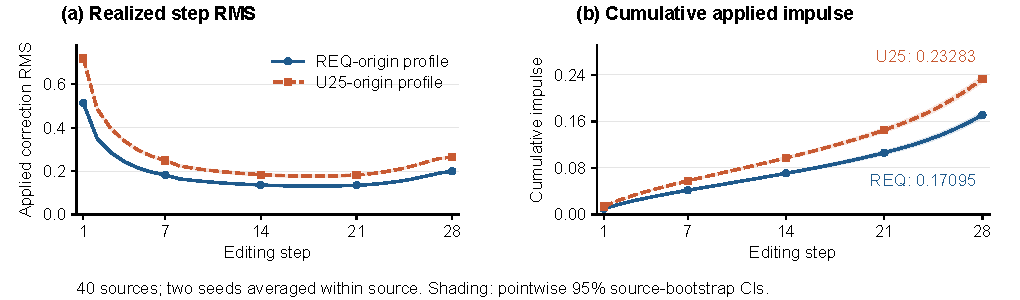
\includegraphics[width=\textwidth]{figures/profiles.pdf}
\caption{Actual RMS and cumulative magnitude profiles, averaged over source/seed groups. Replay-controlled arms follow their designated native anchor. The two profile origins are observed trajectories, not a universal scalar dose law. In this cohort U25 has a larger RMS at every anchor-comparison step.}
\label{fig:profiles}
\end{figure*}

\subsection{Measured profile separation}
Mean cumulative magnitude is $I_R=0.17094737$ (95\% CI $[0.16535783,0.17628020]$) and $I_U=0.23283413$ ($[0.22674989,0.23874031]$). Their paired difference is $0.06188676$ ($[0.05969371,0.06407954]$). The ratio of means $I_U/I_R$ is 1.3620: U25 applies 36.2\% more cumulative correction relative to native REQ. Conversely, $I_R/I_U=0.734202$: REQ applies 73.42\% of U25's cumulative correction, or 26.58\% less relative to U25. These percentages describe cumulative RMS magnitude. This comparison is specific to the 40-source cohort; the historical benchmark's corresponding U25-relative-to-request increase was 32.5\%.

All 80 source/seed anchor pairs satisfy $b_i^U>b_i^R$ at every one of 28 steps. The smallest and largest stepwise differences are 0.02498 and 0.25727. Profile origin is nevertheless the experimental factor: it changes a complete time sequence, including shape as well as cumulative magnitude.

\begin{table*}[!t]
\centering\small
\caption{Same-cohort decomposition of the native preservation-LPIPS difference. Components use shared bootstrap resamples. These are marginal intervals, with no additional hypothesis family.}
\label{tab:paths}
\begin{tabular}{lrr}
\toprule
Component & Mean difference & 95\% CI\\
\midrule
Native REQ $-$ U25 & $+0.03621$ & $[+0.03043,+0.04224]$\\
Path 1: allocation, REQ $-$ GLB-R & $-0.00996$ & $[-0.01389,-0.00639]$\\
Path 1: profile, GLB-R $-$ U25 & $+0.04617$ & $[+0.03934,+0.05378]$\\
Path 2: profile, REQ $-$ REQ-U & $+0.04624$ & $[+0.04015,+0.05251]$\\
Path 2: allocation, REQ-U $-$ U25 & $-0.01003$ & $[-0.01531,-0.00511]$\\
Allocation interaction (uniform minus request origin) & $-0.00007$ & $[-0.00376,+0.00372]$\\
\bottomrule
\end{tabular}
\end{table*}

\subsection{Two paths, one observed native difference}
Table~\ref{tab:paths} links the four factorial cells on the same source population. Path 1 changes allocation at the request-origin profile, then changes profile under uniform allocation. Path 2 changes profile under request weighting, then allocation at the uniform-origin profile. Both sum to the observed native difference for each source, not only in the grand mean. The profile term is about $+0.046$ and the allocation term about $-0.010$ in either path. Thus the observed native uniform advantage coexists with a matched-profile request-weighted advantage.

These paths estimate allocation effects conditional on the two native-policy profiles. Each profile intervention changes cumulative magnitude and temporal shape together, so its contribution combines both features and their trajectory consequences. The near-zero interaction estimate has an uncertainty interval spanning zero. Additional fixed or externally supplied profiles would test a wider anchor class.

\section{Computational Cost of Matched Comparisons}
\begin{table}[!t]
\centering\small
\caption{Generation cost for the original six-arm experiment (480 outputs). Nominal branch NFE excludes prerequisite native anchors. Actual incremental NFE and seconds are means in the executed shared-reference order, not isolated end-to-end timings.}
\label{tab:cost}
\begin{tabular}{lrrr}
\toprule
Arm & \shortstack{Branch\\NFE} & \shortstack{Incremental\\NFE} & \shortstack{Seconds/\\output}\\
\midrule
REQ &97&97.000&63.86\\
GLB-R &97&63.000&45.05\\
U25 &91&62.825&44.93\\
REQ-U &97&63.000&45.05\\
SHUF-R &100&68.650&50.11\\
REV-R &97&63.425&45.38\\
\bottomrule
\end{tabular}
\end{table}

The run required 33,432 new transformer evaluations for 480 outputs, versus a nominal sum of 46,320 branch evaluations without the recorded reuse. Recorded savings comprise 11,172 inversion calls, 1,674 probe calls, and 42 source-memory capture calls. A reference-cache miss in one reversed branch accounts for 34 additional calls relative to its usual incremental cost. Average recorded generation time is 49.06 seconds per output. Metric evaluation and export are separate stages.

Controlled branches also require their anchor. Without shared preparation, the branch-plus-anchor nominal totals are 194 for GLB-R, 188 for REQ-U, 197 for SHUF-R, and 194 for REV-R. The incremental value of 63 measures a controlled branch with reusable preparation already available. Table~\ref{tab:cost} reports the computational requirements of the attribution protocol under both accounting conventions.

\section{Magnitude Scaling and Map Specificity}
\label{sec:extension}
\subsection{Coverage and statistical families}
The follow-up contains all $40\times2\times8=640$ planned new outputs and reuses the original 480, giving 14 arms on the same 40 sources. Category counts remain $5,5,5,5,4,4,4,4,4$. New arms were specified after the original results were available; this is a follow-up on the reused cohort. All six native-image metrics are available for every output. Table~\ref{tab:r89-means} reports the complete means.

% Source: evidence_r89/outputs/statistics/arm_summary.csv.
\begin{table*}[!t]
\centering\footnotesize
\caption{All 14 arms on the same 40 sources. Every cell averages seeds 0 and 17 within source, then sources equally. The first six arms reuse the original 480 outputs; the last eight add 640. All metrics use native images.}
\label{tab:r89-means}
\setlength{\tabcolsep}{5pt}
\begin{tabular}{lrrrrrr}
\toprule
Arm & Pres. LPIPS $\downarrow$ & Full LPIPS $\downarrow$ & Pres. MAE $\downarrow$ & DINO $\uparrow$ & Target CLIP $\uparrow$ & Dir. CLIP $\uparrow$ \\
\midrule
REQ & 0.525352 & 0.544935 & 0.123945 & 0.540550 & 0.264348 & 0.128818 \\
GLB-R & 0.535311 & 0.552767 & 0.126580 & 0.539594 & 0.264653 & 0.129743 \\
U25 & 0.489139 & 0.504496 & 0.105122 & 0.554525 & 0.266477 & 0.135701 \\
REQ-U & 0.479111 & 0.497375 & 0.102306 & 0.553974 & 0.264684 & 0.129120 \\
SHUF-R & 0.526513 & 0.545218 & 0.125079 & 0.538751 & 0.264801 & 0.129966 \\
REV-R & 0.557491 & 0.571900 & 0.138823 & 0.534889 & 0.267309 & 0.134429 \\
\midrule
Global, $0.7b^U$ & 0.540118 & 0.557918 & 0.129818 & 0.538398 & 0.265604 & 0.130742 \\
Request, $0.7b^U$ & 0.531859 & 0.550672 & 0.127155 & 0.538988 & 0.264442 & 0.129428 \\
Global, $1.3b^U$ & 0.432972 & 0.447076 & 0.084485 & 0.574237 & 0.264536 & 0.135803 \\
Request, $1.3b^U$ & 0.420611 & 0.437718 & 0.082238 & 0.577019 & 0.261224 & 0.124262 \\
SOURCE-R & 0.532885 & 0.549682 & 0.128033 & 0.544714 & 0.266882 & 0.133953 \\
SHUF2-R & 0.527264 & 0.545805 & 0.124856 & 0.538385 & 0.264619 & 0.128581 \\
SHUF2-RAW & 0.526332 & 0.544767 & 0.125029 & 0.540492 & 0.264277 & 0.128087 \\
REV-HIST-R & 0.549425 & 0.564450 & 0.133941 & 0.540373 & 0.265857 & 0.132352 \\
\bottomrule
\end{tabular}
\end{table*}


The main family comprises four comparisons---request versus global at $\beta=0.7$ and $1.3$, REQ versus SOURCE-R, and REQ versus SHUF2-R---crossed with preservation LPIPS and directional CLIP (Holm8). The sensitivity family crosses eight comparisons with all six outcomes (Holm48). Tables~\ref{tab:r89-all48-1}--\ref{tab:r89-all48-2} report all 48 rows and identify every main-family test. The original primary/secondary gate and Holm30 family remain as specified in the six-arm study.

Both seeds are averaged before source pairing. The follow-up uses 20,000 category-stratified source bootstraps (PCG64, seed 89002), preserving the nine category counts and using marginal 95\% percentile intervals. Two-sided sign flips use $10^6$ Monte Carlo assignments (seed 89001), absolute source-difference sums, tolerance $10^{-14}$, and $(k+1)/(10^6+1)$. The same resampling indices and sign assignments are used across complete-source contrasts. These tests use the sign-symmetry assumption stated above; the intervals are marginal and the Holm values adjust the specified test families.

% Source: evidence_r89/outputs/statistics/contrasts.csv; archived tests, no rerun.
\begin{table*}[!t]
\centering
\begin{minipage}{\textwidth}
\fontsize{8}{9.2}\selectfont
\caption{Complete follow-up: all 48 tests, part 1/2. Differences are first arm minus second arm, with 40 paired sources after averaging two seeds.}
\label{tab:r89-all48-1}
\setlength{\tabcolsep}{3pt}
\renewcommand{\arraystretch}{1.05}
\begin{tabularx}{\linewidth}{@{}l r >{\centering\arraybackslash}X r r r r@{}}
\toprule
Metric & $\Delta$ & Marginal 95\% CI & $p_{\rm MC}$ & Holm8 & Holm48 & $n_-/n_0/n_+$ \\
\midrule
\multicolumn{7}{@{}l}{\textbf{Request $-$ Global, $\beta=0.7$ at the U25 profile}} \\
Pres. LPIPS $\downarrow$ & $-0.00826$ & $[-0.01188,\,-0.00486]$ & $5.40\!\times\!10^{-5}$ & $4.32\!\times\!10^{-4}$ & $0.002268$ & 29/0/11 \\
Dir. CLIP $\uparrow$ & $-0.00131$ & $[-0.00644,\,+0.00370]$ & $0.667506$ & $1$ & $1$ & 18/0/22 \\
Target CLIP $\uparrow$ & $-0.00116$ & $[-0.00313,\,+0.00088]$ & $0.330797$ & \textemdash & $1$ & 27/0/13 \\
Full LPIPS $\downarrow$ & $-0.00725$ & $[-0.01095,\,-0.00390]$ & $1.48\!\times\!10^{-4}$ & \textemdash & $0.006068$ & 33/0/7 \\
DINO $\uparrow$ & $+0.00059$ & $[-0.00689,\,+0.00826]$ & $0.889035$ & \textemdash & $1$ & 20/0/20 \\
Pres. MAE $\downarrow$ & $-0.00266$ & $[-0.00426,\,-0.00086]$ & $0.012380$ & \textemdash & $0.445680$ & 32/0/8 \\
\midrule
\multicolumn{7}{@{}l}{\textbf{Request $-$ Global, $\beta=1.3$ at the U25 profile}} \\
Pres. LPIPS $\downarrow$ & $-0.01236$ & $[-0.01896,\,-0.00570]$ & $0.001838$ & $0.011028$ & $0.068006$ & 28/0/12 \\
Dir. CLIP $\uparrow$ & $-0.01154$ & $[-0.02042,\,-0.00329]$ & $0.025672$ & $0.128360$ & $0.847175$ & 25/0/15 \\
Target CLIP $\uparrow$ & $-0.00331$ & $[-0.00671,\,+0.00008]$ & $0.072296$ & \textemdash & $1$ & 19/0/21 \\
Full LPIPS $\downarrow$ & $-0.00936$ & $[-0.01601,\,-0.00313]$ & $0.012895$ & \textemdash & $0.445680$ & 26/0/14 \\
DINO $\uparrow$ & $+0.00278$ & $[-0.00911,\,+0.01541]$ & $0.707576$ & \textemdash & $1$ & 22/0/18 \\
Pres. MAE $\downarrow$ & $-0.00225$ & $[-0.00419,\,-0.00008]$ & $0.076918$ & \textemdash & $1$ & 29/0/11 \\
\midrule
\multicolumn{7}{@{}l}{\textbf{REQ $-$ SOURCE-R}} \\
Pres. LPIPS $\downarrow$ & $-0.00753$ & $[-0.01091,\,-0.00428]$ & $1.94\!\times\!10^{-4}$ & $0.001358$ & $0.007760$ & 31/0/9 \\
Dir. CLIP $\uparrow$ & $-0.00513$ & $[-0.01082,\,+0.00022]$ & $0.149117$ & $0.513103$ & $1$ & 22/0/18 \\
Target CLIP $\uparrow$ & $-0.00253$ & $[-0.00452,\,-0.00057]$ & $0.028776$ & \textemdash & $0.892055$ & 25/0/15 \\
Full LPIPS $\downarrow$ & $-0.00475$ & $[-0.00724,\,-0.00225]$ & $8.54\!\times\!10^{-4}$ & \textemdash & $0.033306$ & 29/0/11 \\
DINO $\uparrow$ & $-0.00416$ & $[-0.01104,\,+0.00314]$ & $0.284515$ & \textemdash & $1$ & 23/0/17 \\
Pres. MAE $\downarrow$ & $-0.00409$ & $[-0.00611,\,-0.00175]$ & $0.001536$ & \textemdash & $0.058368$ & 35/0/5 \\
\midrule
\multicolumn{7}{@{}l}{\textbf{REQ $-$ SHUF2-R}} \\
Pres. LPIPS $\downarrow$ & $-0.00191$ & $[-0.00409,\,+0.00038]$ & $0.128276$ & $0.513103$ & $1$ & 30/0/10 \\
Dir. CLIP $\uparrow$ & $+0.00024$ & $[-0.00376,\,+0.00417]$ & $0.914406$ & $1$ & $1$ & 18/0/22 \\
Target CLIP $\uparrow$ & $-0.00027$ & $[-0.00156,\,+0.00106]$ & $0.712868$ & \textemdash & $1$ & 20/0/20 \\
Full LPIPS $\downarrow$ & $-0.00087$ & $[-0.00226,\,+0.00050]$ & $0.284439$ & \textemdash & $1$ & 21/0/19 \\
DINO $\uparrow$ & $+0.00217$ & $[-0.00254,\,+0.00709]$ & $0.450438$ & \textemdash & $1$ & 21/0/19 \\
Pres. MAE $\downarrow$ & $-0.00091$ & $[-0.00167,\,-0.00026]$ & $0.012604$ & \textemdash & $0.445680$ & 28/0/12 \\
\bottomrule
\end{tabularx}
\par\smallskip
{\raggedright Holm8 covers preservation LPIPS and directional CLIP for the four comparisons in part 1; dashes mark tests outside that family. Holm48 covers both parts jointly. Intervals use 20,000 paired category-stratified source bootstraps (seed 89002). Two-sided Monte Carlo sign flips use $10^6$ assignments (seed 89001) and $(k+1)/(10^6+1)$; values near $10^{-6}$ are rounded, not zero. Counts distinguish negative, exactly zero, and positive archived source differences. Arrows give preferred metric direction.\par}
\end{minipage}
\end{table*}

% Source: evidence_r89/outputs/statistics/contrasts.csv; archived tests, no rerun.
\begin{table*}[!t]
\centering
\begin{minipage}{\textwidth}
\fontsize{8}{9.2}\selectfont
\caption{Complete follow-up: all 48 tests, part 2/2. Differences are first arm minus second arm, with 40 paired sources after averaging two seeds.}
\label{tab:r89-all48-2}
\setlength{\tabcolsep}{3pt}
\renewcommand{\arraystretch}{1.05}
\begin{tabularx}{\linewidth}{@{}l r >{\centering\arraybackslash}X r r r r@{}}
\toprule
Metric & $\Delta$ & Marginal 95\% CI & $p_{\rm MC}$ & Holm8 & Holm48 & $n_-/n_0/n_+$ \\
\midrule
\multicolumn{7}{@{}l}{\textbf{SHUF-R $-$ SHUF2-R}} \\
Pres. LPIPS $\downarrow$ & $-0.00075$ & $[-0.00235,\,+0.00080]$ & $0.442511$ & \textemdash & $1$ & 17/12/11 \\
Dir. CLIP $\uparrow$ & $+0.00139$ & $[-0.00003,\,+0.00291]$ & $0.104824$ & \textemdash & $1$ & 14/12/14 \\
Target CLIP $\uparrow$ & $+0.00018$ & $[-0.00063,\,+0.00103]$ & $0.728116$ & \textemdash & $1$ & 12/12/16 \\
Full LPIPS $\downarrow$ & $-0.00059$ & $[-0.00131,\,+0.00012]$ & $0.153001$ & \textemdash & $1$ & 19/12/9 \\
DINO $\uparrow$ & $+0.00037$ & $[-0.00273,\,+0.00344]$ & $0.829416$ & \textemdash & $1$ & 13/12/15 \\
Pres. MAE $\downarrow$ & $+0.00022$ & $[+0.00006,\,+0.00041]$ & $0.044007$ & \textemdash & $1$ & 9/12/19 \\
\midrule
\multicolumn{7}{@{}l}{\textbf{SHUF2-R $-$ SHUF2-RAW}} \\
Pres. LPIPS $\downarrow$ & $+0.00093$ & $[-0.00024,\,+0.00236]$ & $0.275891$ & \textemdash & $1$ & 19/0/21 \\
Dir. CLIP $\uparrow$ & $+0.00049$ & $[-0.00077,\,+0.00181]$ & $0.599366$ & \textemdash & $1$ & 17/0/23 \\
Target CLIP $\uparrow$ & $+0.00034$ & $[-0.00020,\,+0.00091]$ & $0.322353$ & \textemdash & $1$ & 19/0/21 \\
Full LPIPS $\downarrow$ & $+0.00104$ & $[+0.00022,\,+0.00203]$ & $0.026462$ & \textemdash & $0.847175$ & 18/0/22 \\
DINO $\uparrow$ & $-0.00211$ & $[-0.00432,\,-0.00006]$ & $0.098898$ & \textemdash & $1$ & 23/0/17 \\
Pres. MAE $\downarrow$ & $-0.00017$ & $[-0.00042,\,+0.00004]$ & $0.334532$ & \textemdash & $1$ & 20/0/20 \\
\midrule
\multicolumn{7}{@{}l}{\textbf{REQ $-$ REV-HIST-R}} \\
Pres. LPIPS $\downarrow$ & $-0.02407$ & $[-0.03136,\,-0.01727]$ & $1.00\!\times\!10^{-6}$ & \textemdash & $4.80\!\times\!10^{-5}$ & 35/0/5 \\
Dir. CLIP $\uparrow$ & $-0.00353$ & $[-0.01118,\,+0.00321]$ & $0.425758$ & \textemdash & $1$ & 22/0/18 \\
Target CLIP $\uparrow$ & $-0.00151$ & $[-0.00380,\,+0.00087]$ & $0.360569$ & \textemdash & $1$ & 23/0/17 \\
Full LPIPS $\downarrow$ & $-0.01952$ & $[-0.02568,\,-0.01378]$ & $1.00\!\times\!10^{-6}$ & \textemdash & $4.80\!\times\!10^{-5}$ & 35/0/5 \\
DINO $\uparrow$ & $+0.00018$ & $[-0.01196,\,+0.01203]$ & $0.977964$ & \textemdash & $1$ & 23/0/17 \\
Pres. MAE $\downarrow$ & $-0.01000$ & $[-0.01349,\,-0.00637]$ & $2.00\!\times\!10^{-5}$ & \textemdash & $8.60\!\times\!10^{-4}$ & 36/0/4 \\
\midrule
\multicolumn{7}{@{}l}{\textbf{REV-R $-$ REV-HIST-R}} \\
Pres. LPIPS $\downarrow$ & $+0.00807$ & $[+0.00466,\,+0.01224]$ & $3.00\!\times\!10^{-6}$ & \textemdash & $1.32\!\times\!10^{-4}$ & 6/0/34 \\
Dir. CLIP $\uparrow$ & $+0.00208$ & $[-0.00299,\,+0.00862]$ & $0.670725$ & \textemdash & $1$ & 20/0/20 \\
Target CLIP $\uparrow$ & $+0.00145$ & $[-0.00061,\,+0.00373]$ & $0.283664$ & \textemdash & $1$ & 18/0/22 \\
Full LPIPS $\downarrow$ & $+0.00745$ & $[+0.00441,\,+0.01143]$ & $1.00\!\times\!10^{-6}$ & \textemdash & $4.80\!\times\!10^{-5}$ & 5/0/35 \\
DINO $\uparrow$ & $-0.00548$ & $[-0.01305,\,+0.00267]$ & $0.227393$ & \textemdash & $1$ & 28/0/12 \\
Pres. MAE $\downarrow$ & $+0.00488$ & $[+0.00361,\,+0.00619]$ & $1.00\!\times\!10^{-6}$ & \textemdash & $4.80\!\times\!10^{-5}$ & 2/0/38 \\
\bottomrule
\end{tabularx}
\par\smallskip
{\raggedright Holm8 covers preservation LPIPS and directional CLIP for the four comparisons in part 1; dashes mark tests outside that family. Holm48 covers both parts jointly. Intervals use 20,000 paired category-stratified source bootstraps (seed 89002). Two-sided Monte Carlo sign flips use $10^6$ assignments (seed 89001) and $(k+1)/(10^6+1)$; values near $10^{-6}$ are rounded, not zero. Counts distinguish negative, exactly zero, and positive archived source differences. Arrows give preferred metric direction.\par}
\end{minipage}
\end{table*}


Three of eight main-family tests pass Holm8, all on preservation LPIPS: request versus global at $\beta=0.7$ ($\Delta=-0.008259$, adjusted $p=0.000432$), at $\beta=1.3$ ($-0.012361$, $0.011028$), and REQ versus SOURCE-R ($-0.007533$, $0.001358$). Their source win counts are 29, 28, and 31 of 40. In Holm48, ten tests pass: preservation/full LPIPS for the $\beta=0.7$ and source-rank comparisons, and preservation/full LPIPS plus preservation MAE for each comparison with histogram-preserving reversal. The $\beta=1.3$ preservation-LPIPS Holm48 value is 0.068006. CLIP and DINO outcomes have no Holm48 rejection. For $\beta=1.3$, the directional-CLIP difference is $-0.011541$ with marginal interval $[-0.020421,-0.003289]$ and Holm8 $p=0.128360$.

\subsection{Scaling a fixed temporal profile}
Four new arms apply request/global directions at $b_i=\beta b_i^U$, for $\beta=0.7$ and $1.3$; U25 and REQ-U supply the reused $\beta=1$ cells. This changes magnitude while holding the U25 temporal shape fixed. Preservation LPIPS favors request at all three scales, with mean differences $-0.008259$, $-0.010028$, and $-0.012361$. Table~\ref{tab:beta} supplies the corresponding native pixel distances. Raising $\beta$ reduces preservation, edit-region, and full-image pixel departure at both increments for all 40 sources in each direction. Edit-region MAE quantifies source departure; the semantic outcomes are reported separately in the six-metric tables.

% Sources: analysis/records/beta_grid.csv and paired_summary.csv.
\begin{table*}[!t]
\centering\footnotesize
\caption{Native pixel distances for the complete fixed-shape scale sweep, 40 sources. Edit-region MAE measures departure from the source. The $\beta=1$ rows reuse U25 and REQ-U.}
\label{tab:beta}
\begin{tabular}{crrrrrr}
\toprule
 & \multicolumn{3}{c}{Preservation MAE} & \multicolumn{2}{c}{Edit-region MAE} & Lower pres. MAE\\
$\beta$ & Global & Request & Request $-$ Global & Global & Request & for request\\
\midrule
0.7 & 0.129818 & 0.127155 & $-0.002663$ & 0.161579 & 0.167119 & 32/40 \\
1.0 & 0.105122 & 0.102306 & $-0.002816$ & 0.136714 & 0.145197 & 30/40 \\
1.3 & 0.084485 & 0.082238 & $-0.002247$ & 0.114712 & 0.125018 & 29/40 \\
\bottomrule
\end{tabular}
\end{table*}


Figure~\ref{fig:r89-operating-maps} shows the six complete-cohort operating points and the source-level distribution of map correlations.


\subsection{Source ranks, histograms, and donor perturbations}
The four map controls replay the original request profile $b^R$. SOURCE-R uses the native source-prompt velocity, with memory hooks off and guidance 3.5, at the same three reference states as the correct request probes. For the unpacked 16-channel velocity $v_j^s(x)$ on the $64\times64$ grid, its score is
\begin{equation}
S(x)=\frac{1}{3}\sum_{j=1}^{3}\sqrt{\frac{1}{16}\sum_{c=1}^{16}[v_{j,c}^s(x)]^2}.
\end{equation}
Stable ascending $S$ ranks receive ascending sorted correct-$P$ values: $P_{\rm src}(\pi_S(k))=P_{(k)}$. The ranking uses source image/text only; the assigned histogram comes from the correct request map. SOURCE-R then applies
\begin{equation}
\widehat c_i^{\rm src}=b_i^R\frac{P_{\rm src}\odot c_i}{\RMS(P_{\rm src}\odot c_i)}.
\end{equation}
Thus source-velocity channel RMS determines the spatial ranks, while the target-derived histogram and the request-dependent native anchor remain fixed. This control changes spatial ranking while retaining those two request-derived components.
% Definition: code/generation.py:87--88; code/runtime_base/r89_maps.py:6--37; engine.py:278--287.

SHUF2-R selects the same-category donor at cyclic offset $+2$ in case-ID order, evaluates its target on the recipient's reference states, and rank matches its weights to the correct histogram. SHUF2-RAW retains that donor map's raw values. REV-HIST-R assigns ascending correct-$P$ values to descending stable correct-$P$ ranks. The final generation prompt is the recipient's correct target in every arm.

% Source: analysis/records/map_strength_summary.csv; 64x64 scalar maps.
\begin{table*}[!t]
\centering\footnotesize
\caption{Map perturbations relative to the correct request map: seed averages followed by 40-source averages. Relative $L_2$ is $\|P_a-P\|_2/\|P\|_2$; sorted MAE compares sorted map values. These describe scalar weight maps.}
\label{tab:map-controls}
\begin{tabular}{lrrrr}
\toprule
Control & Pearson $r$ & Spearman $\rho$ & Relative $L_2$ & Sorted MAE\\
\midrule
SOURCE-R & 0.116115 & 0.110832 & 0.341908 & 0.000000 \\
SHUF2-R & 0.780937 & 0.765779 & 0.165598 & 0.000000 \\
SHUF2-RAW & 0.781829 & 0.765785 & 0.167846 & 0.020915 \\
REV-HIST-R & $-0.893027$ & $-0.999988$ & 0.508826 & 0.000000 \\
\bottomrule
\end{tabular}
\end{table*}


% These two figure files are replaced by the coordinated full-40-source figure update.
\begin{figure*}[!t]
\centering
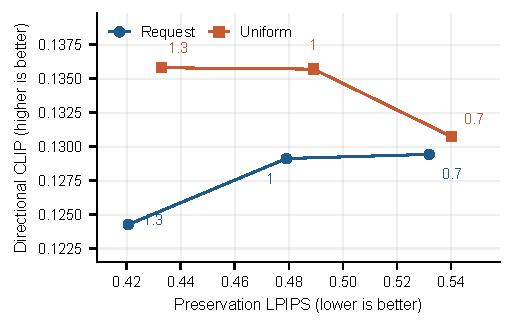
\includegraphics[width=0.49\textwidth]{figures/beta_operating_points.pdf}\hfill
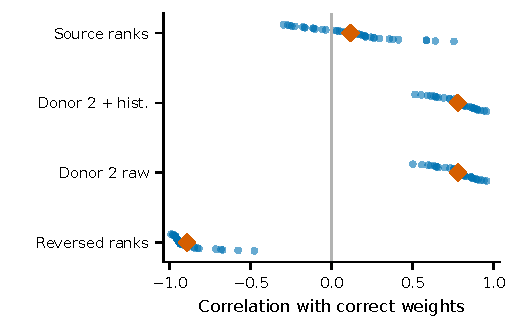
\includegraphics[width=0.49\textwidth]{figures/mapcontrolcorrelation.pdf}
\caption{Complete 40-source follow-up. Left: preservation LPIPS versus directional CLIP for the six $\beta\times$direction operating points; each mean averages the two seeds within source, then all sources equally. The $\beta=1$ points reuse U25 and REQ-U. Right: Pearson correlations between each control's scalar weight map and the correct request map, averaged over the two seeds within each source.}
\label{fig:r89-operating-maps}
\end{figure*}

Figure~\ref{fig:r89-map-examples} shows the map controls for the fixed flower and boy examples.
\begin{figure*}[!t]
\centering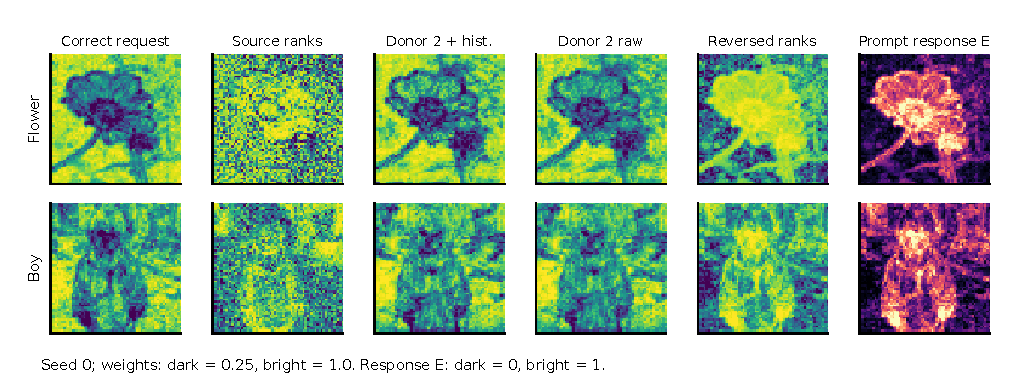
\includegraphics[width=.87\textwidth]{figures/map_controls_full.pdf}
\caption{Two fixed sources, seed 0. Columns 1--5 show correct-request, source-rank, histogram-matched/raw second-donor, and reversed-rank protection weights on a shared $[0.25,1]$ color scale; larger $P$ gives stronger protection. Column 6 shows prompt response $E$ on its own $[0,1]$ color scale.}
\label{fig:r89-map-examples}
\end{figure*}


SOURCE-R, SHUF2-R, and REV-HIST-R preserve all 4,096 sorted correct-map values exactly in each of 80 source/seed records (maximum absolute sorted-value difference zero). Their mean Pearson correlations with the correct map are 0.116115, 0.780937, and $-0.893027$, respectively. The reversal's Spearman correlation is $-0.999988$, including tied values. These scalar-map perturbations retain a large difference in strength between source ranks, donor ranks, and reversed ranks (Table~\ref{tab:map-controls}).

Correct REQ minus REV-HIST-R preservation LPIPS is $-0.024073$; the corresponding MAE difference is $-0.009996$. Thus the reversal effect persists with the correct histogram. Correct REQ minus SHUF2-R preservation LPIPS is $-0.001912$ (30/40 lower), with marginal interval $[-0.004089,0.000376]$ and Holm8 $p=0.513103$. For 12/40 sources the second donor repeats both the first donor's case and target string; 28 supply distinct donor targets, and none repeats the recipient's correct target. The 12 repeated-donor sources tie on native pixel scores to $10^{-12}$. Second-minus-first donor preservation MAE is $-0.000223$ across all sources and $-0.000318$ among the 28 distinct donors. Histogram matching minus the raw second-donor map changes MAE by $-0.000173$, with 20 lower and 20 higher source values. Together with the first donor's correlation of 0.783719 and REQ--SHUF-R LPIPS difference of $-0.00116$ (Holm-adjusted $p=1.0$ across 30 tests), these results leave correct-request specificity unresolved. Correlated maps under wrong requests do not identify generic foreground saliency: donor perturbations retain source structure and request-derived components, and no independent saliency baseline is evaluated.

\subsection{Native boundary and mask sensitivity}
The native audit re-evaluated the original 480 outputs under four masks, producing 1,920 valid mask/output records. Original-mask preservation LPIPS and independent full-image LPIPS agree exactly with their archived values. The forced one-pixel frame adds zero edited pixels for every source, and the reconstructed original and official masks coincide on all 40 sources. The mask convention therefore contributes zero measured discrepancy in this cohort.

For preservation mask $W$, interior variants retain pixels whose Euclidean distance to the nonpreserved region exceeds 8 or 16 pixels; the image exterior is padded with zero. The excluded 0--8 and 0--16 bands average 15.19\% and 29.13\% of the preserved area (ranges 6.81--43.92\% and 13.59--85.20\%). Each variant weights the same whole-image spatial LPIPS map. The changed support quantifies boundary sensitivity while retaining the network's original receptive fields.

% Source: evidence_r89/outputs/r88_native/native_paired_summary.csv.
\begin{table*}[!t]
\centering\footnotesize
\caption{Native-image preservation-LPIPS sensitivity on the original 480 outputs. All summaries average two seeds within each of 40 sources. Parentheses count sources with lower first-arm LPIPS; the interaction has no preferred direction. These are descriptive mask sensitivities.}
\label{tab:r89-native-boundary}
\begin{tabular}{lrrr}
\toprule
Contrast & Original $=$ official & Preserved interior $>8$ px & Preserved interior $>16$ px\\
\midrule
REQ-U $-$ U25 & $-0.010028$ (31/40) & $-0.010882$ (30/40) & $-0.011208$ (29/40) \\
REQ $-$ GLB-R & $-0.009959$ (33/40) & $-0.010315$ (32/40) & $-0.010560$ (32/40) \\
REQ $-$ SHUF-R & $-0.001161$ (25/40) & $-0.001184$ (25/40) & $-0.001090$ (24/40) \\
REQ $-$ REV-R & $-0.032139$ (37/40) & $-0.032860$ (37/40) & $-0.032947$ (38/40) \\
Native REQ $-$ U25 & $+0.036214$ (1/40) & $+0.036282$ (1/40) & $+0.036356$ (1/40) \\
Direction-by-profile interaction & $-0.000069$ & $-0.000567$ & $-0.000648$ \\
\bottomrule
\end{tabular}
\end{table*}


Both matched-direction effects remain negative in the preserved interiors: REQ-U minus U25 changes from $-0.010028$ to $-0.011208$ at 16 pixels; REQ minus GLB-R changes from $-0.009959$ to $-0.010560$. The native unequal-profile REQ-minus-U25 difference remains positive ($+0.036214$ to $+0.036356$). Table~\ref{tab:r89-native-boundary} retains the other controls and interaction, using descriptive source means and wins.

Official edited-area fractions average 32.38\% (range 1.11--92.61\%). Their unadjusted Pearson/Spearman correlations with preservation-LPIPS differences are 0.2175/0.2747 for REQ-U minus U25 and 0.2159/0.1289 for REQ minus GLB-R. The four fixed edited-area bins $[0,.25)$, $[.25,.5)$, $[.5,.75)$, and $[.75,1]$ contain 15, 17, six, and two sources; both contrasts have negative means in every bin. These summaries describe area dependence; perimeter and joint boundary-complexity effects were not measured.

\paragraph{Pixel-score provenance.}
Reported preservation MAE is the recorded \texttt{bg\_mae}: native RGB/255 absolute error, computed in float64 and weighted by the complement of the evaluation edit mask. All 640 follow-up records agree exactly with their metric/evaluation-table entries, and all 480 reused background scores agree with the original archive. The native audit's separate \texttt{preserve\_rgb\_mae} uses float32 $[-1,1]$ tensors followed by division by two; its original-mask maximum difference from recorded MAE is $3.64\times10^{-8}$. Eroded-mask variants use a different support. All arm means and inferential tables retain the original recorded MAE field and the full 40-source population.

\subsection{Complete execution measurements}
All $640\times28=17{,}920$ controlled steps use the designated scaled same-source/seed anchor, with zero difference between target RMS and $\beta$ times anchor RMS, and identical step sizes and scheduler values. Maximum actual-to-target absolute and relative RMS errors are $1.79\times10^{-7}$ and $2.31\times10^{-7}$, respectively; maximum relative cumulative-magnitude error is $3.44\times10^{-8}$. Mean cumulative magnitudes at $0.7b^U$, $b^U$, and $1.3b^U$ are 0.162984, 0.232834, and 0.302684; the map controls replay $I_R=0.170947$.
% Numeric source: analysis/records/rms_step_values.csv and rms_record_audit.csv.
% Exact maxima: absolute 1.7881393432617188e-7; relative 2.3083061395634208e-7; cumulative relative 3.4417862952495219e-8.
% All 17,920 archived r86_relative_rms_error values equal abs(actual_rms-r86_target_rms)/r86_target_rms; maximum discrepancy 0.

% Source: analysis/records/timing_nfe_summary.csv; observed synchronized wall time.
\begin{table*}[!t]
\centering\footnotesize
\caption{Complete eight-arm follow-up cost, 80 outputs per row. Seconds and incremental NFE reflect the executed cache/reuse order. Nominal branch NFE excludes prerequisite anchors; the last column adds their nominal cost.}
\label{tab:r89-cost}
\begin{tabular}{lrrrr}
\toprule
Arm & Seconds/output & Incremental NFE/output & Nominal branch NFE & Branch + anchor NFE\\
\midrule
Global, $0.7b^U$ & 43.48 & 62.6500 & 97 & 188 \\
Request, $0.7b^U$ & 82.63 & 91.0000 & 97 & 188 \\
Global, $1.3b^U$ & 43.86 & 62.3875 & 97 & 188 \\
Request, $1.3b^U$ & 44.12 & 62.9125 & 97 & 188 \\
SOURCE-R & 44.99 & 65.6500 & 97 & 194 \\
SHUF2-R & 57.58 & 68.6250 & 100 & 197 \\
SHUF2-RAW & 43.70 & 62.7375 & 100 & 197 \\
REV-HIST-R & 44.17 & 62.9125 & 97 & 194 \\
\bottomrule
\end{tabular}
\end{table*}


The 640 records sum to 43,110 actual incremental transformer evaluations, compared with 62,560 nominal branch evaluations and 122,720 nominal branch-plus-anchor evaluations (Table~\ref{tab:r89-cost}). Synchronized job time totals 32,362.65 seconds (8.990 job-hours). Request at $0.7b^U$ includes 28 inversion calls per record in this execution order; SHUF2-RAW reuses donor preparation. Nested stage timers overlap and are reported separately from job time.

% Inlined scientific content; r91_followup.tex is no longer an active include.
\section{Seed Variation, Spatial Placement, and Protection Floors}
\label{sec:r91}
These controls ask whether the conditional allocation contrast persists across generation noise, whether the correct histogram alone accounts for it, and how the spatial floor affects joint outcomes. They address different parts of the argument: seed replication concerns the cohort mean, permutations concern spatial organization, and floor changes concern operating-point selection.
\subsection{Paired seed, permutation, and floor design}
The design reuses the same 40 sources: seeds 1, 2, and 3 cross REQ, GLB-R, U25, and REQ-U; two cell permutations are evaluated for each source at seeds 0/17; and floors 0 and 0.5 are evaluated on a fixed 20-source subset at seeds 0/17. This plan was fixed after the primary analyses and before these outcomes.

The added seeds construct their own native request and uniform anchors, then cross the allocation rules with these anchors. The map and floor interventions instead replay the exact archived profiles for seeds 0 and 17. No editor, resolution, integration schedule, guidance, memory rule, or source-selection criterion changes. Reference computations are cached; each arm evaluates the correction at its own evolving state.

\paragraph{Cell permutations}
For each source/seed pair, RAND-A and RAND-B independently permute all 4,096 scalar entries of the correct protection map. Permutation keys combine the source identifier, generation seed, and draw identifiers 9001 or 9002; each map remains fixed over all integration steps. The maps preserve the correct target-derived histogram exactly, use the original request-origin magnitude profile $b^R$, and retain the correct generation prompt. Averaging the two draws defines RAND in the paired analysis. Their mean Pearson correlation with the correct map is 0.00035; maximum sorted-value difference is zero across all 160 maps. This intervention disrupts spatial arrangement and smoothness together. It retains target-derived values and anchor information, so its contrast measures organized placement rather than isolated semantic request specificity.

\paragraph{Protection floor}
The floor experiment uses $P_f=f+(1-f)(1-E)$ at $f\in\{0,0.25,0.5\}$ and replays $b^U$ for each arm. The $f=0.25$ reference reuses REQ-U; U25 provides the uniform direction at the same profile. The 20 sources are selected by a fixed hash order, with three from each of categories 0 and 1 and two from each remaining category, independently of image scores. All 80 new maps match the specified formula exactly. A zero floor permits zero weights but every recorded weighted residual has positive RMS, so stepwise replay remains feasible. Floor changes alter relative spatial allocation while keeping applied magnitude fixed.

\paragraph{Evaluation method}
Native RGB outputs use the LPIPS, CLIP, and regional-MAE definitions above. Paired outcomes share sources, masks, and processing. Software versions, coverage, and numerical reproduction checks are consolidated in Section~\ref{sec:reproducibility}.

\subsection{Statistical families and estimands}
The primary follow-up is the added-three-seed allocation effect on the reused 40-source cohort. Original-two-seed and pooled-five-seed estimates remain separate. Seeds, and permutation draws where applicable, are averaged within source before inference. Marginal intervals use 20,000 category-stratified source bootstraps. The frozen calculation uses one million Monte Carlo sign flips and the plus-one correction; the sign-symmetry assumption is unchanged. The analysis uses a deterministic PCG64 stream initialized at 91013. Intervals condition on the specified seeds and preserve the original category mixture.

The two added-seed preservation contrasts form Holm2. The three REQ/SOURCE-R/GLB-R versus RAND comparisons form one Holm3 family for preservation LPIPS and a separate Holm3 family for directional CLIP. The two added floors versus floor 0.25, crossed with LPIPS and directional CLIP, form Holm4. For this 20-source floor family, we subsequently enumerated all $2^{20}=1{,}048{,}576$ sign assignments to refine the near-threshold Monte Carlo result. The statistic, four contrasts, source pairing, and Holm family are unchanged. Exact two-sided probabilities count assignments with an absolute mean at least as large as observed, with numerical tolerance $10^{-15}$; exhaustive enumeration uses no plus-one correction. Table~\ref{tab:r91-floor} reports exact floor probabilities and the original bootstrap intervals. For floor 0 directional CLIP, the raw probability is $13022/1048576=0.012419$, giving Holm4 $0.049675$; the frozen Monte Carlo values are $0.012374$ and $0.049496$. The exact test can be reconstructed from the 20 paired source means in the floor arms of \path{source_correction_and_blending/replication_scores.csv}. Floor-versus-U25, edit-MAE, pooled-seed, and added-seed joint-outcome intervals are descriptive. Additional joint-outcome bootstraps use seed 91114; LPIPS intervals reuse the planned replication intervals.

\begin{table*}[!t]
\centering\small
\caption{Original two-seed estimates, added three-seed replication, and pooled five-seed sensitivity. Original and pooled rows are descriptive in this table. The added pair forms Holm2. Recomputed original bootstrap bounds can vary slightly from the archived bounds because the bootstrap stream differs.}
\label{tab:r91-replication}
\begin{tabular}{llrrrrr}
\toprule
Contrast & Outcome & Sources & Mean & 95\% CI & Raw $p$ & Holm $p$\\
\midrule
REQ-U $-$ U25 (original two) & LPIPS & 40 & $-0.0100$ & $[-0.0151, -0.0051]$ & --- & ---\\
REQ-U $-$ U25 (new three) & LPIPS & 40 & $-0.0114$ & $[-0.0171, -0.0059]$ & 0.000404 & 0.000404\\
REQ-U $-$ U25 (pooled five) & LPIPS & 40 & $-0.0109$ & $[-0.0158, -0.0062]$ & --- & ---\\
REQ $-$ GLB-R (original two) & LPIPS & 40 & $-0.0100$ & $[-0.0139, -0.0064]$ & --- & ---\\
REQ $-$ GLB-R (new three) & LPIPS & 40 & $-0.0114$ & $[-0.0157, -0.0074]$ & 0.000002 & 0.000004\\
REQ $-$ GLB-R (pooled five) & LPIPS & 40 & $-0.0108$ & $[-0.0147, -0.0072]$ & --- & ---\\
\bottomrule
\end{tabular}
\end{table*}

\begin{table*}[!t]
\centering\small
\caption{Per-seed preservation-LPIPS contrasts on 40 sources. Marginal source-bootstrap intervals condition on the indicated seed. Negative sources count paired differences below zero.}
\label{tab:r91-seeds}
\begin{tabular}{llrrr}
\toprule
Contrast & Seed & Mean & 95\% CI & Negative sources\\
\midrule
REQ-U $-$ U25 & 0 & $-0.0126$ & $[-0.0204, -0.0051]$ & 29/40\\
REQ-U $-$ U25 & 17 & $-0.0074$ & $[-0.0118, -0.0032]$ & 25/40\\
REQ-U $-$ U25 & 1 & $-0.0120$ & $[-0.0183, -0.0062]$ & 27/40\\
REQ-U $-$ U25 & 2 & $-0.0120$ & $[-0.0177, -0.0064]$ & 30/40\\
REQ-U $-$ U25 & 3 & $-0.0103$ & $[-0.0189, -0.0025]$ & 29/40\\
REQ $-$ GLB-R & 0 & $-0.0107$ & $[-0.0154, -0.0064]$ & 33/40\\
REQ $-$ GLB-R & 17 & $-0.0092$ & $[-0.0150, -0.0045]$ & 31/40\\
REQ $-$ GLB-R & 1 & $-0.0094$ & $[-0.0140, -0.0052]$ & 30/40\\
REQ $-$ GLB-R & 2 & $-0.0116$ & $[-0.0157, -0.0076]$ & 34/40\\
REQ $-$ GLB-R & 3 & $-0.0132$ & $[-0.0203, -0.0071]$ & 34/40\\
\bottomrule
\end{tabular}
\end{table*}

\begin{table*}[!t]
\centering\small
\caption{Added-seed outcomes averaged over seeds 1, 2, and 3 within each of 40 sources. These joint-outcome summaries are descriptive with marginal source-bootstrap intervals; no additional hypothesis-test family is introduced.}
\label{tab:r91-joint}
\begin{tabular}{llrr}
\toprule
Contrast & Outcome & Mean & 95\% CI\\
\midrule
REQ-U $-$ U25 & Pres. LPIPS & $-0.0114$ & $[-0.0171, -0.0059]$\\
REQ-U $-$ U25 & Target CLIP & $-0.0004$ & $[-0.0025, +0.0016]$\\
REQ-U $-$ U25 & Dir. CLIP & $+0.0007$ & $[-0.0049, +0.0057]$\\
REQ-U $-$ U25 & Edit MAE & $+0.0081$ & $[+0.0059, +0.0102]$\\
REQ-U $-$ U25 & Pres. MAE & $-0.0030$ & $[-0.0047, -0.0012]$\\
REQ $-$ GLB-R & Pres. LPIPS & $-0.0114$ & $[-0.0157, -0.0074]$\\
REQ $-$ GLB-R & Target CLIP & $-0.0021$ & $[-0.0043, +0.0000]$\\
REQ $-$ GLB-R & Dir. CLIP & $+0.0005$ & $[-0.0043, +0.0052]$\\
REQ $-$ GLB-R & Edit MAE & $+0.0054$ & $[+0.0037, +0.0072]$\\
REQ $-$ GLB-R & Pres. MAE & $-0.0035$ & $[-0.0052, -0.0017]$\\
\bottomrule
\end{tabular}
\end{table*}

\begin{table*}[!t]
\centering\small
\caption{Cell-permutation comparisons, 40 sources and two original seeds. RAND averages two independently keyed permutations within each source/seed. LPIPS and directional CLIP each form a separate three-test Holm family. Intervals are marginal.}
\label{tab:r91-permutation}
\begin{tabular}{llrrrrr}
\toprule
Contrast & Outcome & Sources & Mean & 95\% CI & Raw $p$ & Holm $p$\\
\midrule
REQ $-$ RAND & LPIPS & 40 & $-0.0135$ & $[-0.0186, -0.0090]$ & 0.000001 & 0.000003\\
GLB-R $-$ RAND & LPIPS & 40 & $-0.0036$ & $[-0.0051, -0.0022]$ & 0.000003 & 0.000006\\
SOURCE-R $-$ RAND & LPIPS & 40 & $-0.0060$ & $[-0.0094, -0.0030]$ & 0.000636 & 0.000636\\
REQ $-$ RAND & Dir. CLIP & 40 & $-0.0013$ & $[-0.0063, +0.0034]$ & 0.6399 & 1.0000\\
GLB-R $-$ RAND & Dir. CLIP & 40 & $-0.0004$ & $[-0.0025, +0.0017]$ & 0.7305 & 1.0000\\
SOURCE-R $-$ RAND & Dir. CLIP & 40 & $+0.0038$ & $[-0.0004, +0.0083]$ & 0.1941 & 0.5822\\
\bottomrule
\end{tabular}
\end{table*}

\begin{table*}[!t]
\centering\small
\caption{Protection-floor comparisons on the prespecified 20-source subset and two original seeds. The four floor-versus-0.25 LPIPS/directional-CLIP contrasts form Holm4; their probabilities enumerate all $2^{20}$ sign assignments, refining the frozen Monte Carlo calculation. Original bootstrap intervals are retained. Comparisons with U25 and edit-MAE contrasts are descriptive. All arms replay the same original uniform-origin profile.}
\label{tab:r91-floor}
\begin{tabular}{llrrrrr}
\toprule
Contrast & Outcome & Sources & Mean & 95\% CI & Raw $p$ & Holm $p$\\
\midrule
Floor 0 $-$ REQ-U & LPIPS & 20 & $-0.0009$ & $[-0.0042, +0.0024]$ & 0.7419 & 1.0000\\
Floor 0.5 $-$ REQ-U & LPIPS & 20 & $+0.0014$ & $[-0.0016, +0.0043]$ & 0.4641 & 1.0000\\
Floor 0 $-$ U25 & LPIPS & 20 & $-0.0137$ & $[-0.0251, -0.0023]$ & --- & ---\\
REQ-U $-$ U25 & LPIPS & 20 & $-0.0128$ & $[-0.0216, -0.0040]$ & --- & ---\\
Floor 0.5 $-$ U25 & LPIPS & 20 & $-0.0114$ & $[-0.0177, -0.0051]$ & --- & ---\\
Floor 0 $-$ REQ-U & Dir. CLIP & 20 & $+0.0085$ & $[+0.0034, +0.0141]$ & 0.0124 & 0.0497\\
Floor 0.5 $-$ REQ-U & Dir. CLIP & 20 & $-0.0013$ & $[-0.0057, +0.0031]$ & 0.7643 & 1.0000\\
Floor 0 $-$ U25 & Dir. CLIP & 20 & $+0.0033$ & $[-0.0033, +0.0102]$ & --- & ---\\
REQ-U $-$ U25 & Dir. CLIP & 20 & $-0.0051$ & $[-0.0121, +0.0018]$ & --- & ---\\
Floor 0.5 $-$ U25 & Dir. CLIP & 20 & $-0.0064$ & $[-0.0148, +0.0017]$ & --- & ---\\
Floor 0 $-$ REQ-U & Edit MAE & 20 & $+0.0072$ & $[+0.0054, +0.0089]$ & --- & ---\\
Floor 0.5 $-$ REQ-U & Edit MAE & 20 & $-0.0042$ & $[-0.0055, -0.0030]$ & --- & ---\\
\bottomrule
\end{tabular}
\end{table*}

\begin{table}[!t]
\centering\small
\caption{Joint operating points for the 20-source floor subset, averaging two seeds within source. REQ-U uses floor 0.25. LPIPS is lower-is-better; directional CLIP measures text response; edit MAE measures pixel change.}
\label{tab:r91-floor-points}
\begin{tabular}{lrrr}
\toprule
Arm & Pres. LPIPS & Dir. CLIP & Edit MAE\\
\midrule
Floor 0 & 0.466610 & 0.151506 & 0.156506\\
REQ-U & 0.467490 & 0.143009 & 0.149266\\
Floor 0.5 & 0.468882 & 0.141719 & 0.145036\\
U25 & 0.480261 & 0.148157 & 0.141277\\
\bottomrule
\end{tabular}
\end{table}

\subsection{What the controls establish}
The added seeds reproduce the cohort-mean conditional preservation contrast; randomized maps show that equal RMS can support harmful as well as beneficial allocations; and the floor comparison links spatial redistribution to editing response. Together these results distinguish the allocation estimate from the choice of a complete editing configuration.
\paragraph{Seed replication on the same sources}
Averaging seeds 1, 2, and 3 gives REQ-U minus U25 preservation LPIPS $-0.01145$, CI $[-0.01714,-0.00592]$, Holm2 $p=0.000404$. REQ minus GLB-R gives $-0.01140$, CI $[-0.01572,-0.00735]$, Holm2 $p=0.000004$. Both profile-specific means are negative in each of the five observed seeds (Table~\ref{tab:r91-seeds}). Pooled five-seed means are $-0.01088$ and $-0.01082$, with marginal intervals $[-0.01582,-0.00618]$ and $[-0.01468,-0.00721]$. Both summaries reuse the same 40 sources; added seeds test sensitivity to generation noise, and five-seed pooling is descriptive.

The added-seed primary edit-MAE contrast is $+0.00808$, CI $[0.00592,0.01024]$, alongside a directional-CLIP contrast $+0.00075$, CI $[-0.00486,0.00572]$. Increased pixel change accompanies the preservation improvement again, while the directional-CLIP point difference changes sign relative to the original two seeds. The replicated joint observation is lower preservation error with greater edit-region departure; departure includes unintended changes, and directional-CLIP differences remain uncertain in both seed sets. Table~\ref{tab:r91-joint} reports the corresponding target CLIP and preservation MAE as well as both profile origins.

\paragraph{Individual-source variation}
For the primary contrast, 14 sources favor request weighting under all five seeds, one favors uniform under all five, and 25 have mixed signs. The five-seed source mean favors request weighting on 28/40 sources. Pairwise sign disagreements range from 9/40 to 17/40 across all ten seed pairs (Table~\ref{tab:r91-signs}); the original pair has 16/40. The five-seed mixed-sign count has more opportunities to change sign and is not a directly comparable instability rate. Figure~\ref{fig:r91-heterogeneity} shows every source/seed cell. The replicated cohort mean coexists with substantial source-specific variation.

\paragraph{Randomized placement and source-derived ranks}
Correct REQ improves over RAND by $0.01355$ preservation LPIPS: difference $-0.01355$, CI $[-0.01859,-0.00899]$, Holm3 $p=0.000003$. GLB-R also improves over RAND by $0.00359$ (CI $[-0.00514,-0.00217]$, Holm3 $p=0.000006$), and SOURCE-R improves by $0.00601$ (CI $[-0.00942,-0.00299]$, Holm3 $p=0.000636$). All three corresponding directional-CLIP intervals include zero (Table~\ref{tab:r91-permutation}). The correct-map versus RAND directional-CLIP difference is $-0.00133$, CI $[-0.00630,0.00336]$.

Relative to GLB-R, the SOURCE-R-to-REQ gain ratio remains 0.244, whereas the randomized-map ratio is $-0.360$: randomized weighting has higher preservation error than uniform correction at the same profile. SOURCE-R replaces spatial ranks with source-only velocity ranks while retaining the target-derived weight histogram and native request anchor. The ratios summarize mean outcome contrasts; 0.244 therefore measures the retained gain under that particular rank replacement, with no interpretation as a fraction or lower bound of source information.

The preserved histogram and matched RMS accommodate both beneficial and harmful spatial patterns. Cell permutation jointly disrupts smoothness and alignment with image structure, so the evidence concerns spatial organization as a whole. Highly correlated wrong-request maps yield uncertain contrasts against the correct request. Separating correct-request specificity from generic spatial structure remains open within these controls.

\paragraph{Floor sensitivity and joint outcomes}
On the fixed 20-source subset, floors 0, 0.25, and 0.5 give preservation LPIPS 0.46661, 0.46749, and 0.46888; its U25 reference gives 0.48026. Floor 0 minus U25 is $-0.0137$ LPIPS with descriptive 95\% interval $[-0.0251,-0.0023]$, and $+0.0033$ directional CLIP with descriptive interval $[-0.0033,0.0102]$. Floor 0.25 minus U25 directional CLIP is $-0.0051$ ($[-0.0121,0.0018]$). These paired comparisons use 20 sources, separate from the 40-source scale curves. Floor 0 has favorable joint point estimates; CLIP uncertainty leaves Pareto superiority unestablished.

Relative to floor 0.25, floor 0 changes LPIPS by $-0.00088$ (CI $[-0.00416,0.00242]$), and floor 0.5 by $+0.00139$ (CI $[-0.00155,0.00430]$); both four-test Holm-adjusted $p$ values are 1.0. Floor 0 raises directional CLIP by $+0.00850$ (CI $[0.00336,0.01407]$; exact four-test Holm-adjusted $p=0.0497$) and edit MAE by $+0.00724$ (CI $[0.00541,0.00888]$). The adjusted CLIP result is close to the 0.05 threshold. Floor 0.5 gives CLIP $-0.00129$ (CI $[-0.00567,0.00310]$; adjusted $p=1.0$) and edit MAE $-0.00423$ (CI $[-0.00545,-0.00295]$). LPIPS intervals spanning zero describe uncertainty, not equivalence.

Under normalized replay, the local multiplier is $b_i^U P_f(x)/\RMS(P_f\odot c_i)$; a weight floor of 0.25 is a relative spatial floor, not an absolute 25\% source correction. Floor 0 permits zero correction at maximum-response locations and changes the normalized direction while holding full-vector stepwise RMS fixed. Regional correction energy can change under this constraint. The result demonstrates floor-sensitive editing response at the tested profile; explaining the high-scale CLIP decline or estimating a floor-zero equal-preservation tradeoff would require further comparisons. Floor 0.25 remains the primary reference, and the fixed-subset outcomes are reported separately from the 40-source scale curves.


\begin{figure*}[!t]
\centering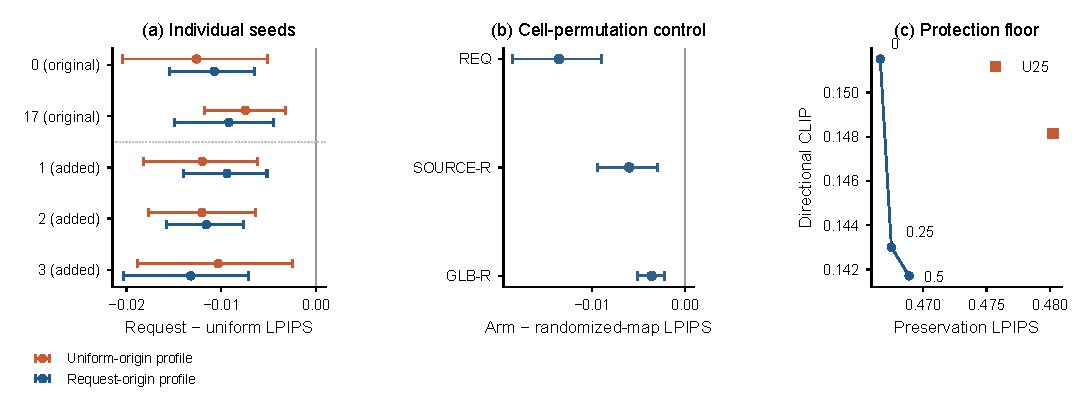
\includegraphics[width=\textwidth]{figures/r91_followup.pdf}
\caption{Seed, placement, and floor controls. (a) Preservation contrasts separately for each of five observed seeds, with marginal 95\% category-stratified source-bootstrap intervals. The dotted line separates original and added seeds. (b) Paired contrasts against the two-draw randomized-map mean, averaging seeds 0 and 17 within 40 sources. All methods share the request-origin magnitude profile; negative favors the named arm. (c) Joint preservation/text-response means on the fixed 20-source floor subset. Labels give protection floors; the square is U25. Segments connect tested points and do not estimate a continuous frontier.}
\label{fig:r91}
\end{figure*}

\begin{table}[!t]
\centering\small
\caption{Opposite-sign source counts for every pair of observed seeds. Pairwise comparisons have equal exposure to seed variation; the event of any sign change over all five seeds is a different summary.}
\label{tab:r91-signs}
\begin{tabular}{lrr}
\toprule
Seed pair & REQ-U--U25 & REQ--GLB-R\\
\midrule
0, 1 & 12/40 & 13/40\\
0, 2 & 17/40 & 11/40\\
0, 3 & 14/40 & 5/40\\
0, 17 & 16/40 & 8/40\\
1, 2 & 9/40 & 10/40\\
1, 3 & 10/40 & 8/40\\
2, 3 & 9/40 & 10/40\\
17, 1 & 12/40 & 11/40\\
17, 2 & 11/40 & 11/40\\
17, 3 & 10/40 & 11/40\\
\bottomrule
\end{tabular}
\end{table}

\begin{figure*}[!t]
\centering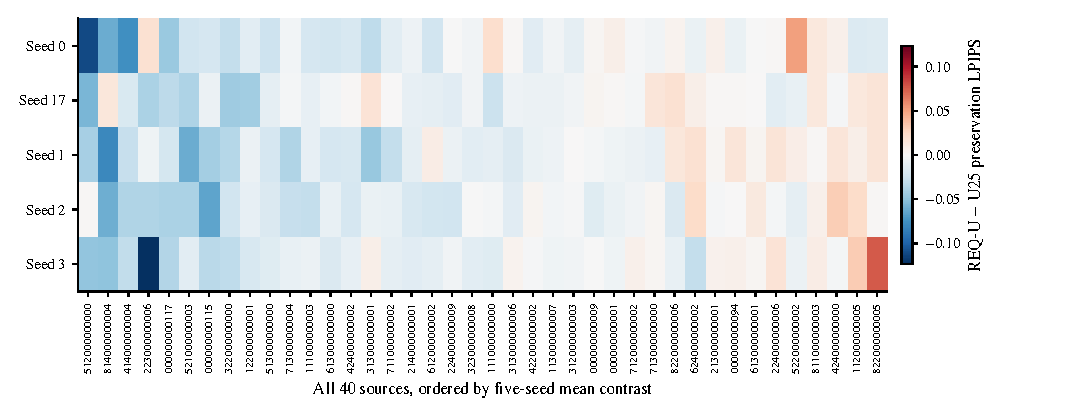
\includegraphics[width=\textwidth]{figures/r91_source_seeds.pdf}
\caption{All source-by-seed primary contrasts. Color denotes REQ-U minus U25 preservation LPIPS under each seed's uniform-origin profile; blue favors request weighting. Columns are sorted by five-seed mean, with a common symmetric color scale. This descriptive view retains all sources and exposes sign changes without selecting a favorable subset.}
\label{fig:r91-heterogeneity}
\end{figure*}


\section{What One-Shot Scalar Calibration Recovers}
\label{sec:scalar-complete}
The completed scalar comparison evaluates a specified one-shot approximation to the uniform-origin correction profile. It characterizes the sequence and allocation contrast produced by a coefficient calculated from native records. We report realized profile errors alongside preservation and editing response.
\subsection{Calibration rule and paired design}
The scalar comparison uses the same 40 sources and seeds 0/17, with one request-weighted output per pair. The coefficient rule and two primary contrasts were fixed before these 80 outcomes, with a fixed sample size and no outcome-based coefficient search.

For each source/seed pair, its native U25 and REQ records at $\lambda=0.25$ give $I_U=\sum_i h_i b_i^U$ and $I_R=\sum_i h_i b_i^R$. Set
\begin{equation}
\lambda_{\rm SC}=0.25\,\frac{I_U}{I_R},\qquad
\widehat c_i^{\rm SC}=\lambda_{\rm SC}P\odot c_i(z_i^{\rm SC}).
\end{equation}
This pair-specific coefficient stays fixed throughout generation, without outcome-score fitting. The map, reference, prompts, seed, memory, scheduler, and precision match the original comparison. Each run recomputes its residual at its own state. The ratio would match cumulative magnitude if the native request run's candidate residual sequence remained fixed; recomputation along SC's own trajectory determines its realized sequence. U25, REQ-U, and native REQ are reused comparison arms. SC minus native REQ measures the change from calibrating the native request-weighted rule. SC minus REQ-U (stepwise) directly compares scalar calibration with replay under the same request-weighted allocation. SC minus U25 and REQ-U minus U25 give the respective allocation comparisons under these two calibration procedures.

Native outputs use the same preservation-LPIPS, CLIP, and regional-MAE definitions as the seed comparison. Table~\ref{tab:r92-results} presents measured outcomes; file coverage is specified in Section~\ref{sec:reproducibility}.

\paragraph{When can one scalar match the full profile?}
For a fixed sequence of nonzero candidate vectors $v_i$ and positive targets $b_i$, a nonnegative constant $\lambda$ satisfies $\RMS(\lambda v_i)=b_i$ at every step exactly when
\begin{equation}
\frac{b_i}{\RMS(v_i)}=\lambda\quad\text{for every }i.
\end{equation}
This follows directly from homogeneity of RMS. With a single intervention at a shared state and a fixed nonzero direction, one admissible scalar suffices. For several steps, the required ratios must coincide. In a rollout, $v_i$ depends on the states induced by the chosen coefficient, so the condition must hold on that coefficient's own realized trajectory. Ratios measured on an earlier trajectory provide a calibration proposal whose realized sequence must be checked. If the operator restricts its coefficient range, the common ratio must also lie within that range. This condition explains what exact matching entails; outcome agreement between approximate calibrations remains an empirical question.

\subsection{Source-level inference}
The sampling unit is the source ($n=40$). Arm means average seeds 0/17 within each source, then weight all sources equally; paired contrasts first subtract matched arms within each source/seed and then use the same averaging order. The frozen primary family contains two two-sided preservation-LPIPS tests: SC--REQ-U and SC--U25, adjusted jointly by Holm2. Monte Carlo sign flips use 1,000,000 assignments and the plus-one estimator $(k+1)/(1{,}000{,}000+1)$, with PCG64 seed 92013. Marginal 95\% intervals use 20,000 category-stratified paired source bootstraps, retaining all 40 sources and planned category counts, conditional on these two seeds. Other outcomes and SC minus native REQ are descriptive. The original gated/expanded families and all original intervals remain unchanged. R92 re-bootstrap intervals for reused contrasts are identified separately and do not replace original intervals.

\paragraph{Trajectory diagnostics and aggregation.}
For each source/seed pair, let $b_i=b_i^U$ be the target U25 RMS, $\widehat b_i=\RMS(\widehat c_i^{\rm SC})$ the actual SC RMS, and $h_i=\sigma_i-\sigma_{i+1}$ the shared integration step size. Define $I=\sum_i h_i b_i=I_U$ and $\widehat I=\sum_i h_i\widehat b_i=I_{\rm SC}$. The four recorded diagnostics are
\begin{align}
e_{\rm cum}&=\frac{\widehat I-I}{I},\\
e_{\rm abs}&=\frac{\sum_i h_i|\widehat b_i-b_i|}{I},\\
e_{\rm max}&=\max_i\frac{|\widehat b_i-b_i|}{b_i},\\
d_{\rm shape}&=\sum_i\left|\frac{h_i\widehat b_i}{\widehat I}-\frac{h_i b_i}{I}\right|.
\end{align}
Here $e_{\rm cum}$ is signed cumulative relative error, $e_{\rm abs}$ is integrated absolute relative error, $e_{\rm max}$ is maximum stepwise relative error, and $d_{\rm shape}$ is normalized temporal-shape L1 distance. The shape distance uses step-size-weighted normalized contributions and the full L1 sum, without a factor of one half. It compares the temporal distribution after normalizing each trajectory by its own cumulative magnitude; $e_{\rm cum}$ separately records the total-magnitude difference. Table~\ref{tab:r92-diagnostics} expresses the first three errors as percentages and the shape distance in dimensionless units. All target RMS values and both cumulative magnitudes are positive in these records.

Each diagnostic is computed separately for each source/seed trajectory, then averaged over seeds 0/17 within source and over the 40 sources equally. Thus the reported mean maximum is the mean of per-trajectory maxima, and the reported relative errors average per-trajectory ratios. Marginal 95\% intervals resample these source means within category, using the 20,000-draw R92 bootstrap described above. The diagnostic definitions follow the generation archive's \path{runtime_base/r92_controls.py}; aggregation and intervals follow \path{analysis/r92/frozen_analyze.py}.

\begin{table*}[!t]
\centering\small
\caption{R92 operating points and paired outcomes, averaged over 40 sources after averaging two seeds within source. LPIPS and MAE are distances; directional CLIP is higher-is-better. Differences are first minus second. Intervals are marginal 95\% R92 bootstrap intervals. Only the two designated LPIPS contrasts have Holm2-adjusted tests; all other entries are descriptive. The native REQ edit MAE comes from the original R88 per-output evaluation (80 records); other entries retain the frozen R92 analysis.}
\label{tab:r92-results}
\begin{tabular}{lrrr}
\toprule
Arm & Preservation LPIPS & Directional CLIP & Edit MAE\\
\midrule
REQ & 0.525352 & 0.128818 & 0.164571\\
SC & 0.485271 & 0.130216 & 0.148146\\
REQ-U & 0.479111 & 0.129120 & 0.145197\\
U25 & 0.489139 & 0.135701 & 0.136714\\
\bottomrule
\end{tabular}
\par\medskip
\begin{tabular}{llrrr}
\toprule
Contrast & Outcome & Difference & 95\% CI & Holm2 $p$\\
\midrule
SC $-$ REQ-U & Pres. LPIPS & $+0.006160$ & $[0.004714,0.007704]$ & 0.000002\\
SC $-$ U25 & Pres. LPIPS & $-0.003868$ & $[-0.008473,0.000544]$ & 0.139348\\
SC $-$ native REQ & Pres. LPIPS & $-0.040081$ & $[-0.045489,-0.034913]$ & ---\\
REQ-U $-$ U25 & Pres. LPIPS & $-0.010028$ & $[-0.015216,-0.005077]$ & ---\\
SC $-$ REQ-U & Dir. CLIP & $+0.001096$ & $[-0.000932,0.003041]$ & ---\\
SC $-$ U25 & Dir. CLIP & $-0.005486$ & $[-0.013101,0.001853]$ & ---\\
SC $-$ native REQ & Dir. CLIP & $+0.001397$ & $[-0.005522,0.007703]$ & ---\\
REQ-U $-$ U25 & Dir. CLIP & $-0.006581$ & $[-0.014074,0.000548]$ & ---\\
SC $-$ REQ-U & Edit MAE & $+0.002950$ & $[0.002393,0.003552]$ & ---\\
SC $-$ U25 & Edit MAE & $+0.011432$ & $[0.008966,0.013956]$ & ---\\
REQ-U $-$ U25 & Edit MAE & $+0.008482$ & $[0.006089,0.010953]$ & ---\\
\bottomrule
\end{tabular}
\end{table*}

\begin{table}[!t]
\centering\small
\caption{R92 scalar diagnostics: source means and marginal 95\% category-stratified bootstrap intervals. Percentage errors refer to the U25 target. Original native-dose intervals elsewhere retain their archived values; these are R92 re-bootstrap summaries.}
\label{tab:r92-diagnostics}
\begin{tabular}{lrr}
\toprule
Quantity & Mean & 95\% CI\\
\midrule
Native $I_R$ & 0.170947 & $[0.165457,0.176301]$\\
Native $I_U$ & 0.232834 & $[0.226776,0.238774]$\\
Realized $I_{\rm SC}$ & 0.223068 & $[0.217443,0.228499]$\\
$\lambda_{\rm SC}$ & 0.341670 & $[0.337521,0.345874]$\\
Cumulative error (\%) & $-4.1603$ & $[-4.7910,-3.5798]$\\
Integrated abs. error (\%) & 4.5022 & $[3.9231,5.1298]$\\
Max. step rel. error (\%) & 7.7051 & $[6.8728,8.6074]$\\
Temporal-shape L1 & 0.021214 & $[0.018551,0.024026]$\\
\bottomrule
\end{tabular}
\end{table}


\subsection{Realized profiles and outcomes}
SC's mean coefficient is 0.341670; mean realized cumulative magnitude is 0.223068 versus native U25's 0.232834. The source-mean relative cumulative error is $-4.1603\%$ (CI $[-4.7910,-3.5798]\%$), negative for all 40 sources. Normalized temporal-shape L1 is 0.021214 (CI $[0.018551,0.024026]$). Integrated absolute relative error is 4.5022\%, and the mean maximum stepwise relative error is 7.7051\% (Table~\ref{tab:r92-diagnostics}). Figure~\ref{fig:r92-scalar}(a) displays the realized stepwise deviations. Thus this one-shot coefficient leaves both a residual dose difference and a different temporal shape.

SC minus native REQ preservation LPIPS is $-0.040081$ (CI $[-0.045489,-0.034913]$), with all 40 source differences negative. SC--U25 is $-0.003868$ (CI $[-0.008473,0.000544]$; Holm2 $p=0.139348$), with 22/40 differences negative. Scalar calibration thus changes the native ranking in point estimate; the interval spans zero, leaving the sign statistically unresolved. No equivalence margin was prespecified. The direct SC--REQ-U (stepwise) contrast is $+0.006160$ (CI $[0.004714,0.007704]$; Holm2 $p=0.000002$), positive for 38/40 sources. Since both allocation comparisons use U25 as their reference, this direct paired contrast quantifies how much the estimated allocation effect changes between scalar calibration and stepwise replay.

SC--REQ-U directional CLIP is $+0.001096$ (CI $[-0.000932,0.003041]$); edit-region MAE is $+0.002950$ (CI $[0.002393,0.003552]$), positive for all 40 sources. The latter measures pixel change, including unintended changes, rather than instruction success. Table~\ref{tab:r92-results} reports the joint operating points and descriptive contrasts. Figure~\ref{fig:r92-scalar}(c) retains all 40 paired source effects.

The direct comparison establishes that this one-shot calibration and prescribed-profile replay yield different quantitative allocation estimates. SC has higher preservation LPIPS and edit-region MAE than REQ-U, with an uncertain directional-CLIP difference. Its realized cumulative magnitude, temporal shape, and ensuing trajectory feedback change together. These measurements leave two explanations open: residual total-magnitude mismatch may account for much of the gap, or temporal allocation and state feedback may remain consequential after totals are matched.

An existing-data scale check illustrates the residual-dose explanation. The descriptive request-weighted slope from the three-scale fit is $-0.796337$ LPIPS per unit cumulative magnitude (Section~\ref{sec:next-steps-20261106}). Multiplying its absolute value by $0.232834-0.223068=0.009766$ gives approximately 0.0078 LPIPS, comparable in size to the measured SC--REQ-U gap of 0.006160. This is a cohort-level sensitivity calculation under the fitted response model. Source heterogeneity, temporal shape, and state feedback remain combined; the calculation supplies no causal allocation of the gap.

\paragraph{Realized-total calibration.}
The one-shot rule fixes the coefficient using two previously observed trajectories. A bounded coefficient search targeting the actual total on each candidate's own rollout defines a different comparison. The recorded one-shot trajectories simultaneously change realized total, temporal shape and state feedback. They do not identify how much of the observed LPIPS gap comes from each.

\begin{figure*}[!t]
\centering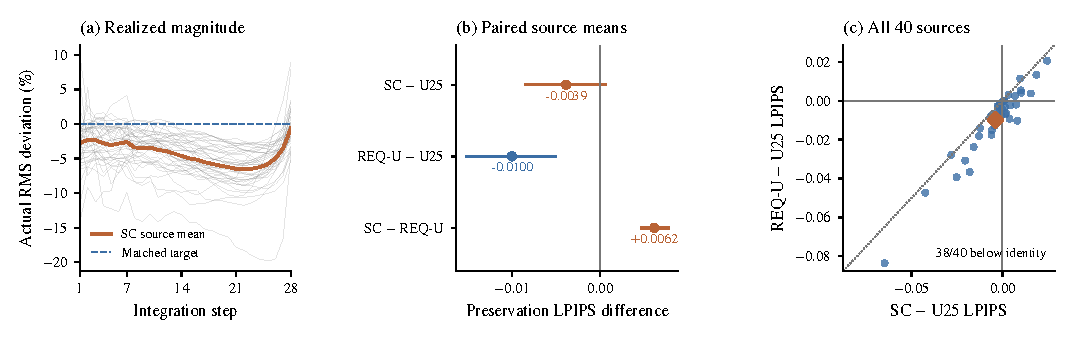
\includegraphics[width=\textwidth]{figures/r92_scalar_summary.pdf}
\caption{Completed one-shot scalar calibration on all 40 sources, averaging seeds 0/17 within source. (a) Relative applied-RMS deviations from the U25 target over 28 steps: gray curves are sources, orange is their mean, and blue zero is the target. (b) Preservation-LPIPS contrasts with marginal 95\% R92 category-stratified source-bootstrap intervals; SC--REQ-U and SC--U25 form the Holm2 family, while reused REQ-U--U25 is descriptive here. These re-bootstrap intervals do not replace the original study's intervals. (c) All source contrasts: SC--U25 on the horizontal axis and REQ-U--U25 on the vertical axis. Thirty-eight of 40 sources lie below identity; the orange diamond is the cohort mean.}
\label{fig:r92-scalar}
\end{figure*}

\begin{figure*}[!t]
\centering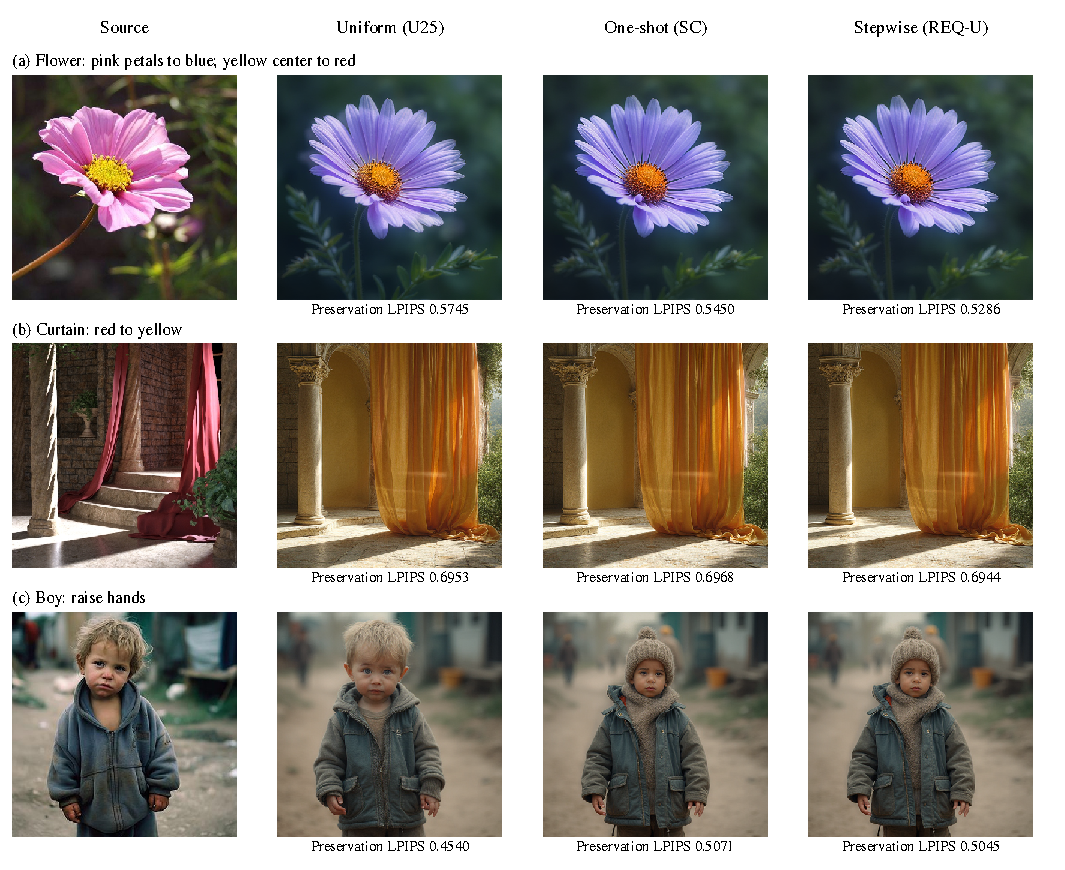
\includegraphics[width=0.96\textwidth]{figures/r92_native_examples.pdf}
\caption{Native $512\times512$ source, U25, SC, and REQ-U images for the three examples in Fig.~\ref{fig:legacy-native}, selected before scalar outcomes: flower 000000000117, curtain 613000000001, and boy 522000000002, all at seed 0. The cases were fixed by the earlier illustrative selection and reused without selection on R92 outcomes. Displayed preservation LPIPS values are seed-0 scores, not the two-seed source means used for inference. Identical full-image views illustrate preservation and requested-edit behavior; these three cases do not estimate success frequency.}
\label{fig:r92-native}
\end{figure*}

\section{Operator Dependence: DirectEdit Blending}
\label{sec:external}
We apply the comparison protocol to the local blend in DirectEdit~\cite{yang2026directedit} using 20 sources from the 40-source cohort, five configurations, and one deterministic run per source (100 outputs). Images are $512\times512$ with 30 steps, inversion/editing guidance 1/2, attention ratio 0.15, four initial V-injection steps, layer ratio zero, and no skipped steps. Official PIE masks are supplied to the editor, unlike the annotation-free routing maps of the main experiment.

Let $y_i$ be the edited latent before blending, $s_i$ the paired source-branch latent, and $m$ the supplied edit mask. Local and global blend directions are $(1-m)\odot(s_i-y_i)$ and $s_i-y_i$. The native local blend has coefficient one; two further anchors use coefficient 0.25. Each matched arm replays the other anchor's actual blend RMS. This intervention is a latent displacement, applied directly without another multiplication by the integration step size. It is measured at the editor's blend operation rather than as the velocity correction in the main paper.

\begin{table}[!t]
\centering\small
\caption{DirectEdit blend application: 20 sources, five arms, one deterministic run per source. Archived native-image pixel means; edit-region MAE measures source departure.}
\label{tab:directedit}
\begin{tabular}{lrr}
\toprule
Configuration & Pres. MAE $\downarrow$ & Edit-region MAE\\
\midrule
Native local, coefficient 1 &0.013399&0.054980\\
Local, coefficient 0.25 &0.014281&0.060152\\
Global, coefficient 0.25 &0.012993&0.017445\\
Local at global profile &0.014101&0.058206\\
Global at local profile &0.017413&0.028829\\
\bottomrule
\end{tabular}
\end{table}

Local minus global preservation MAE is $+0.001108$ at the global-origin profile (2/20 sources lower) and $-0.003132$ at the local-origin profile (14/20 lower). Their local-origin-minus-global-origin interaction is $-0.004240$ (18/20 negative): the direction effect changes sign with profile origin. Table~\ref{tab:next-steps-20261106} adds paired intervals and exact tests. Native local blending at coefficient one improves over local 0.25 by 0.000882, with lower preservation error on all 20 sources.

Original step logs also identify when a replay extrapolates beyond convex blending. With the effective coefficient computed as target blend RMS divided by the candidate direction RMS and a threshold of $1+10^{-6}$, local-at-global exceeds one in 149/600 steps on 10/20 sources (maximum 16.524). Global-at-local exceeds one in 8/600 steps on 1/20 (maximum 3.566). These counts describe the two 30-step replay arms; the reported LPIPS and MAE contrasts use all 20 sources.
The 20-source category counts are $2,2,2,2,2,2,3,2,3$. Selection follows the archived hash ordering with two top-up sources. VAE mode and deterministic inversion give one run per source; seed zero is its identifier. Original MAE scores use native RGB/255 images weighted by $m$ and $1-m$.

\paragraph{Native-image LPIPS and CLIP.}
All 100 native outputs are evaluated against their paired sources. LPIPS uses the same AlexNet-v0.1 weights and whole-image feature extraction as above. Preservation LPIPS weights the spatial map by the area-resampled complement of the supplied edit mask: grayscale masks are nearest-resized to 512 and divided by 255, without thresholding, dilation, or frame exclusion. Full LPIPS uses a separate nonspatial pass. CLIP uses the same checkpoint, processor, exact planned prompts, and normalized-difference score. Implementation identity and evaluation settings appear in Section~\ref{sec:reproducibility}.

Table~\ref{tab:directedit-native-20261106} reports descriptive post hoc estimates with 20,000 category-stratified paired source bootstraps (seed 20261108), shared across arms and metrics. Only marginal 95\% intervals are added; the original MAE Holm6 membership is unchanged. Local-minus-global preservation LPIPS is $+0.037086$ (CI $[0.025736,0.048793]$) at the global origin and $+0.002996$ (CI $[-0.004826,0.011051]$) at the local origin. Both LPIPS point estimates favor global blending; the local-origin interval includes zero. Unlike pixel MAE, LPIPS has no sign reversal. This boundary case shows why crossed-profile comparison should measure sensitivity to the chosen control, with either sign retained. Directional-CLIP point differences favor local at both origins; the local-origin interval also spans zero. GLOBAL\_025 is a near-identity working point (directional CLIP 0.00111; full LPIPS 0.01560). Preservation therefore needs to be read alongside editing response. Operator, mask construction, and configuration change together, so the observed dependence is specific to this combination rather than an isolated operator effect.

% Sources: analysis/directedit_native_20261106/{per_arm_metrics.csv,
% paired_descriptive_ci.csv,evaluation_config.json}.
\begin{table*}[!t]
\centering\footnotesize
\setlength{\tabcolsep}{5pt}
\caption{DirectEdit metrics from all 100 recovered native outputs (20 sources, five arms). Top: source means. Bottom: paired local-minus-global effects at each profile origin and their local-origin-minus-global-origin interaction, with marginal 95\% intervals from 20,000 category-stratified source bootstraps. These are descriptive post hoc summaries; no new $p$ values or Holm family are introduced. Original pixel MAE is retained in Table~\ref{tab:directedit}.}
\label{tab:directedit-native-20261106}
\begin{tabular}{@{}lrrrr@{}}
\toprule
Configuration & Pres. LPIPS $\downarrow$ & Full LPIPS $\downarrow$ & Target CLIP $\uparrow$ & Dir. CLIP $\uparrow$\\
\midrule
Native local, coefficient 1 & 0.039628 & 0.103094 & 0.237792 & 0.077952\\
Local, coefficient 0.25 & 0.052474 & 0.120747 & 0.240882 & 0.084875\\
Global, coefficient 0.25 & 0.014584 & 0.015596 & 0.231284 & 0.001113\\
Local at global profile & 0.051670 & 0.118606 & 0.239640 & 0.086342\\
Global at local profile & 0.049477 & 0.063773 & 0.240979 & 0.047243\\
\midrule
Contrast & \multicolumn{2}{c}{Preservation LPIPS: difference [95\% CI]} & \multicolumn{2}{c}{Directional CLIP: difference [95\% CI]}\\
\midrule
Local $-$ global, global origin & \multicolumn{2}{c}{$+0.037086\;[+0.025736,+0.048793]$} & \multicolumn{2}{c}{$+0.085229\;[+0.050198,+0.121419]$}\\
Local $-$ global, local origin & \multicolumn{2}{c}{$+0.002996\;[-0.004826,+0.011051]$} & \multicolumn{2}{c}{$+0.037632\;[-0.000510,+0.076920]$}\\
Interaction & \multicolumn{2}{c}{$-0.034090\;[-0.046356,-0.021526]$} & \multicolumn{2}{c}{$-0.047597\;[-0.075788,-0.020358]$}\\
\bottomrule
\end{tabular}
\end{table*}


\section{Operating-Point and Map-Alignment Diagnostics}
\label{sec:next-steps-20261106}

\begin{figure}[!t]
\centering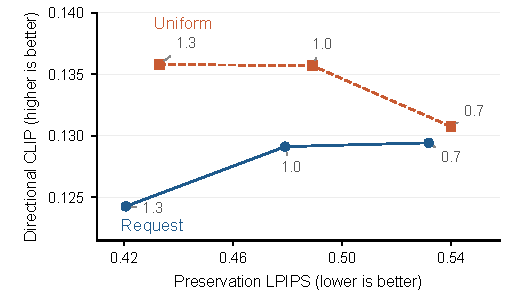
\includegraphics[width=\linewidth]{figures/beta_operating_points_v5.pdf}
\caption{Original-seed joint operating points at three scales of the uniform-origin profile, averaged within 40 sources over seeds 0/17. Labels give $\beta$. Segments connect tested settings; uncertainty and adjusted tests are reported in this section.}
\label{fig:scale-joint}
\end{figure}

These post hoc analyses retain the specified primary, secondary, and sensitivity families. Scale and map summaries average seeds within each of 40 sources; paired category-stratified bootstraps use 20,000 draws (seed 20261106) and marginal 95\% percentile intervals. Table~\ref{tab:next-steps-20261106} groups the results; Fig.~\ref{fig:next-steps-20261106} shows their context. The scale-to-profile calculation uses retained records and adds no hypothesis tests.

\paragraph{Interpolated equal-LPIPS comparison and $\beta$ trends.}
Piecewise-linear curves join the three observed cohort means per direction at $\beta=0.7,1,1.3$. Let $C_G(\ell)$ and $C_R(\ell)$ denote interpolated directional CLIP at preservation LPIPS $\ell$, and $[\ell_-,\ell_+]$ their shared range. The reported average is
\begin{equation}
\overline\Delta_C=\frac{1}{\ell_+-\ell_-}\int_{\ell_-}^{\ell_+}[C_G(\ell)-C_R(\ell)]\,d\ell.
\end{equation}
Over $[0.43297,0.53186]$, this gives $+0.006524$ (unadjusted 95\% CI $[0.0008579,0.0126601]$). Each bootstrap draw recomputes the means, curves, and overlap without extrapolation; all 20,000 draws support this summary. This interval captures source variation conditional on piecewise-linear interpolation. Linearity between the three scales is an assumption, not a validated finding, and no multiplicity adjustment is applied to this post hoc interval. The estimand compares cohort-mean automatic scores with uniform weighting over the LPIPS interval; it differs from a contrast at one common scale and reuses the same observations. Its narrower interval does not supply independent evidence of practical superiority. At fixed LPIPS targets 0.48, 0.50, and 0.52, gaps are $+0.006593$, $+0.005403$, and $+0.003340$, supported by 19,916, 19,222, and 14,959 draws; these points are reported without conditional intervals.

\paragraph{Post hoc equal-response analysis within each source.}
The original three scales per allocation also allow the inverse question: at equal editing response on the same source, which allocation yields lower background LPIPS? We averaged seeds 0/17 within each source, allocation and $\beta\in\{0.7,1,1.3\}$, giving 240 points from 480 archived outputs. We then applied the first-crossing integration and 10,000-draw paired source bootstrap of Section~\ref{sec:sam-scan}, requiring three complete points per curve. At equal directional CLIP, uniform minus request preservation LPIPS is $+0.01280$ [0.00219, 0.02396], positive on 22 and negative on 14 of 36 overlapping sources. The median common width is 0.01286. Four of 40 sources have disjoint ranges: 223000000006, 414000000004, 513000000000 and 822000000005. At equal edit MAE, the difference is $+0.03084$ [0.01970, 0.04235] on 40/40, positive on 33 and negative on seven, median width 0.03184. Neither comparison has missing or point-contact curves. The earlier equal-LPIPS result uses cohort means before interpolation. Here each source supplies its own interval and difference before cohort averaging.

\paragraph{Cumulative magnitude and profile differences.}
The sweep changes cumulative magnitude while retaining each source/seed's uniform-origin temporal shape. Let $\bar L_d(\beta)$ be cohort-mean preservation LPIPS for allocation $d$ at scale $\beta$. The ratio of cohort-mean native magnitudes is $q=\bar I_R/\bar I_U=0.734202$, within the observed interval $[0.7,1]$. A local linear prediction of the profile contrast is
\begin{equation}
\widehat D_d=\frac{1-q}{1-0.7}\big[\bar L_d(0.7)-\bar L_d(1)\big].
\end{equation}
The uniform-rule prediction is 0.045168 versus the observed GLB-R--U25 difference 0.046173; the request-weighted prediction is 0.046735 versus REQ--REQ-U 0.046242. Their prediction-to-observation ratios are 0.978 and 1.011. As fitting sensitivity, ordinary least squares over all three scales gives slopes $-0.766974$ and $-0.796337$ LPIPS per unit cumulative magnitude. Multiplying each slope by $\bar I_R-\bar I_U=-0.061887$ predicts 0.047466 and 0.049283, with ratios 1.028 and 1.066. These are deterministic, post hoc summaries; no additional confidence interval or test is claimed.

The proximity of these predictions to the observed profile differences is consistent with a substantial cumulative-magnitude contribution under the assumed response models. Scaling by $q$ matches only the cohort-mean cumulative magnitude: individual source/seed ratios differ, and the temporal shapes remain uniform-origin. The residuals, 0.001005 and $-0.000493$ for local interpolation, combine any shape contribution with interpolation error, heterogeneous responses, and possible interactions. They therefore neither identify nor bound a temporal-shape effect. The ratios above are model comparisons, not additive percentages of causation. The scale measurements are in \path{source_correction_and_blending/three_scale_points.csv}.

Let $d_\beta$ be the source-paired request-minus-uniform effect. The four post hoc trend tests are $d_{1.3}-d_{0.7}$ and $d_{0.7}-2d_1+d_{1.3}$ for preservation LPIPS and directional CLIP. Two-sided sign flips use 199,999 Monte Carlo assignments (seed 20261107) with the plus-one correction. All four Holm4-adjusted $p$ values exceed 0.05 (panel A). These tests concern the allocation contrast's variation across scales, separately from the magnitude response of either individual rule.

\paragraph{Map alignment and first-donor association.}
AUROC treats the official preservation mask as positive, broadcasts each $64\times64$ scalar weight to its $8\times8$ pixel cell, and excludes the one-pixel image frame. Seed-averaged source means are 0.72054 for correct $P$, 0.49377 for SOURCE-R, 0.67084 for SHUF2-R, and 0.27951 for REV-HIST-R (panel B). These cross-map means describe weight-mask alignment, not a causal dose--response: map construction, smoothness, and residual alignment vary together. Correction-energy allocation also depends on the residual fields.

For the first histogram-matched donor (SHUF1, the original SHUF-R), correct-map Pearson correlation averages 0.783719 across sources (range 0.516335--0.957052). Within this SHUF1 comparison, correlation with the SHUF-R-minus-REQ preservation-LPIPS effect is Pearson $0.013$ and Spearman $-0.093$. The category-centered slope is $0.002347$ per correlation unit (95\% CI $[-0.01215,0.02521]$). This cross-source association provides no causal-mediation estimate.

\paragraph{DirectEdit native-MAE paired inference.}
The 20-source native-MAE contrasts use 20,000 paired category-stratified bootstrap draws (seed 20261108) and two-sided exact sign flips over all $2^{20}$ assignments. A post hoc Holm6 family combines the two local-minus-global profile contrasts and their local-origin-minus-global-origin interaction for background and edit-region MAE (panel C). Background effects change sign across origins, whereas edit-region source departure increases under the local direction at both origins.

% Sources: analysis/next_steps_20261106/{summary.json,analysis_plan.json,
% beta_direction_trend.csv,map_mask_summary.csv,directedit_paired.csv}.
% Existing-data analyses specified after outcomes were observed; old test families retained.
\begin{table*}[!t]
\centering\footnotesize
\setlength{\tabcolsep}{4pt}
\caption{Post-outcome existing-data analyses. All intervals are marginal 95\% category-stratified source-bootstrap intervals (20,000 draws). Panel A uses Monte Carlo sign flips and its own Holm4 family; panel B is descriptive; panel C uses exact $2^{20}$ sign flips and one Holm6 family across three contrasts and two MAE outcomes. $d_\beta$ is request minus global; L--G is local minus global. Interaction is the local-origin contrast minus the global-origin contrast.}
\label{tab:next-steps-20261106}
\begin{tabular}{@{}llrrrr@{}}
\toprule
Outcome / map & Contrast / summary & Estimate & 95\% CI & Unadjusted $p$ & Holm $p$\\
\midrule
\multicolumn{6}{@{}l}{\textit{A. Direction-effect trends: 40 sources, post hoc Holm4}}\\
Preservation LPIPS & $d_{1.3}-d_{0.7}$ & $-0.004102$ & $[-0.009086,+0.000901]$ & 0.16883 & 0.50649\\
Preservation LPIPS & $d_{0.7}-2d_1+d_{1.3}$ & $-0.000564$ & $[-0.005670,+0.004712]$ & 0.853945 & 1\\
Directional CLIP & $d_{1.3}-d_{0.7}$ & $-0.010228$ & $[-0.020135,-0.001055]$ & 0.085145 & 0.34058\\
Directional CLIP & $d_{0.7}-2d_1+d_{1.3}$ & $+0.000308$ & $[-0.013119,+0.014518]$ & 0.97034 & 1\\
\midrule
\multicolumn{6}{@{}l}{\textit{B. Weight-map alignment: 40 sources, official preservation positive}}\\
Correct $P$ & Preservation-mask AUROC & 0.720543 & $[0.661953,0.778988]$ & -- & --\\
SOURCE-R & Preservation-mask AUROC & 0.493773 & $[0.448340,0.540041]$ & -- & --\\
SHUF2-R & Preservation-mask AUROC & 0.670840 & $[0.605631,0.735889]$ & -- & --\\
REV-HIST-R & Preservation-mask AUROC & 0.279506 & $[0.221134,0.338053]$ & -- & --\\
\midrule
\multicolumn{6}{@{}l}{\textit{C. DirectEdit native MAE: 20 paired sources, post hoc Holm6}}\\
Preservation MAE & L--G, global origin & $+0.001108$ & $[+0.000480,+0.001735]$ & 0.0009346 & 0.0028038\\
Preservation MAE & L--G, local origin & $-0.003132$ & $[-0.004748,-0.001402]$ & 0.0060387 & 0.0060387\\
Preservation MAE & Interaction & $-0.004240$ & $[-0.006055,-0.002234]$ & $1.90735\times10^{-5}$ & $7.62939\times10^{-5}$\\
Edit-region MAE & L--G, global origin & $+0.040761$ & $[+0.033406,+0.048068]$ & $3.8147\times10^{-6}$ & $2.28882\times10^{-5}$\\
Edit-region MAE & L--G, local origin & $+0.031323$ & $[+0.025274,+0.037228]$ & $3.8147\times10^{-6}$ & $2.28882\times10^{-5}$\\
Edit-region MAE & Interaction & $-0.009438$ & $[-0.014947,-0.004022]$ & 0.0030174 & 0.0060349\\
\bottomrule
\end{tabular}
\end{table*}


\begin{figure*}[!t]
\centering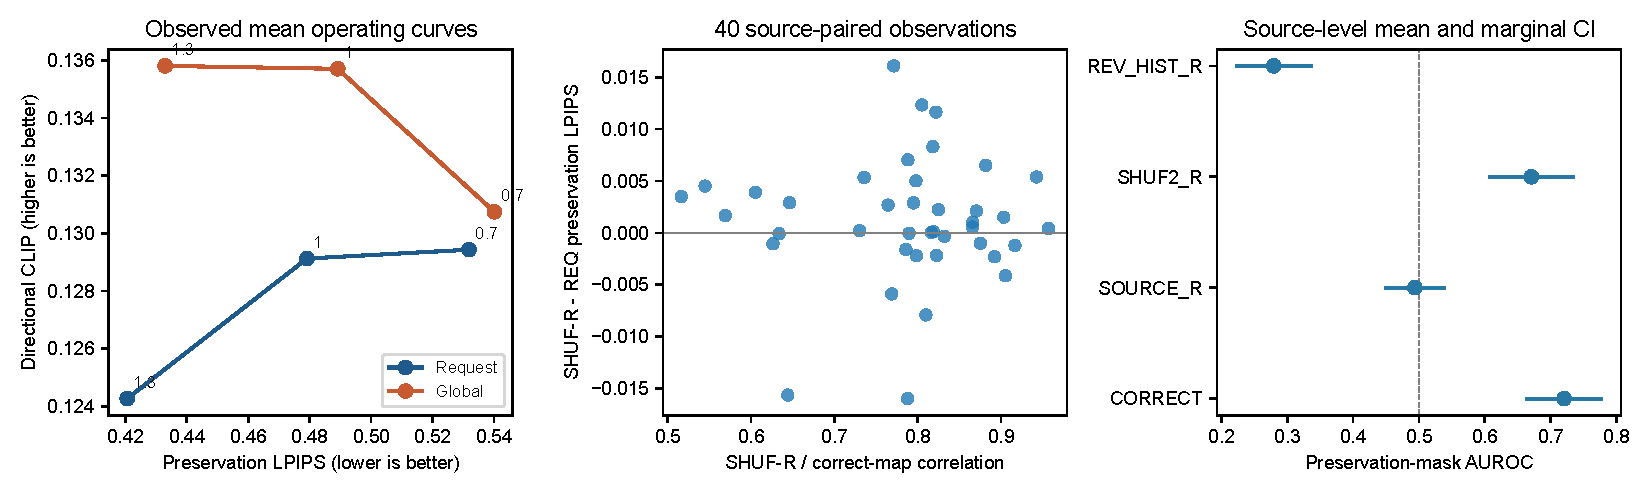
\includegraphics[width=\textwidth]{figures/next_steps_20261106_existing_data_diagnostics.pdf}
\caption{Post-outcome diagnostics from existing data. Left: three observed mean operating points per direction and their linear interpolants. Middle: first-donor (SHUF1/SHUF-R) map correlation versus the paired preservation-LPIPS difference for 40 sources. Right: preservation-mask AUROC means and marginal category-bootstrap intervals; larger scalar weights predict preservation. Each source averages its two seeds.}
\label{fig:next-steps-20261106}
\end{figure*}

\section{Source Robustness and Image Change}
\subsection{Full-cohort source robustness}
This sensitivity check uses automatic metrics on all 40 sources. Trimming removes two observations per tail at 5\% and four per tail at 10\%, giving means $-0.008447$ and $-0.007653$, respectively. Leave-one-source-out means range from $-0.010813$ to $-0.008142$. The two-seed scores for this calculation are in \path{source_correction_and_blending/two_seed_per_output.csv}.

\subsection{Per-seed results and conditional inference}
Table~\ref{tab:r91-seeds} consolidates both original seeds and the three added seeds in one source-bootstrap summary. Among the original seed pair, 24/40 sources have the same nonzero sign and 16 have opposite signs; 19 improve under both. Figure~\ref{fig:r91-heterogeneity} and Table~\ref{tab:r91-signs} extend this view to all five seeds without duplicating the original per-seed table. Intervals describe source variation conditional on each indicated seed.

\subsection{Image change alongside preservation}
The paired image-change scatter in Fig.~\ref{fig:paired-heterogeneity} uses all 160 recovered U25/REQ-U native outputs. RGB error is averaged over the complement of the official preservation mask, then over seeds within source. Cohort edit-region MAE is 0.136714 for U25 and 0.145197 for REQ-U, compared with preservation LPIPS 0.489139 and 0.479111. Thus the aggregate retention gain accompanies greater pixel change inside the edit region. Pixel departure can include artifacts and geometric changes; it is reported alongside directional CLIP and the native visual examples. The scatter is descriptive and does not condition away the effects of source content or task difficulty.

\section{Same-State Norms and Method Correspondence}
\subsection{Recovering the energy-weighted attenuation}
For a nonzero residual, $e_i(P)=\RMS(P\odot c_i)^2/\RMS(c_i)^2$ uses the same residual in both reductions. Archived \texttt{candidate\_global\_rms} and \texttt{current\_correction\_global\_rms} provide these reductions before magnitude matching when calibration and spatial support are global. Coverage includes 80 recovered REQ-U runs and 480 weighted extension runs (15,680 steps). Both reductions use one current-state residual; norms from different trajectories would measure a different quantity.

The time-weighted per-run mean is $\bar e=\sum_i h_i e_i/\sum_i h_i$, followed by seed averaging within source. For correct weights along REQ-U, its source mean is 0.48752, range 0.40968--0.62481. At profile scales 0.7 and 1.3 the corresponding means are 0.49928 and 0.47600. These later-state summaries include trajectory changes. The shared initial state instead gives identical correct-map $e$ across these three runs for each source/seed, with source mean 0.50965 and range 0.34691--0.66296.

For native REQ the original 80 logs provide all 2,240 steps (40 sources, seeds 0/17). The same-state, time-weighted $\bar e$ averages 0.49807 across sources, with source means from 0.42243 to 0.62739. The native REQ value uses the original step logs. The 0.48752 value above belongs to the distinct REQ-U trajectory.

The REQ-U time-weighted value has Pearson correlation 0.0098 with the source-level REQ--GLB-R preservation-LPIPS contrast (95\% category-bootstrap interval $[-0.3251,0.3476]$). Correct-map AUROC has Pearson correlation $-0.2644$ ($[-0.5138,-0.0308]$) and Spearman correlation $-0.2625$ ($[-0.5212,0.0341]$) with that contrast. These descriptive intervals use 20,000 category-stratified source draws, seed 20261112. Geometry and residual-weighted attenuation are different measurements; neither supplies a regional energy decomposition from global norms alone. Source-level AUROC values and paired LPIPS contrasts are in \path{evidence/map_source_values.csv}.

\subsection{Boundary cases and scope of the norm identity}
For $P\equiv p>0$, $e_i(P)=p^2$ and $(P\odot c_i)/\RMS(P\odot c_i)=c_i/\RMS(c_i)$. A constant map can therefore attenuate the unnormalized residual while leaving its normalized direction unchanged. Strict norm reduction requires nonzero residual energy at a location where $P<1$. A nonconstant map with $P=(1,0.5)$ and $c=(1,0)$ gives equality. If $c_i=0$, both unnormalized corrections vanish and $e_i$ is undefined; a positive target norm then cannot be replayed. The positive floor ensures nonzero weighted directions whenever the residual is nonzero in the original experiment. The added zero-floor experiment checks feasibility directly; all recorded replay directions remain nonzero. These identities constrain the instantaneous correction; final image metrics include the integrated target field and decoder.

The RMS attenuation factor is $\sqrt{e_i(P)}$; $e_i(P)$ is its square. For a complete update containing another field $a_i$, the norm of $a_i+P\odot c_i$ also depends on their cross term. The identity therefore motivates measuring the specified intervention at its actual application point. It does not determine the final preservation ranking: randomized spatial placement supplies an observed higher-error case at the same RMS profile.

\subsection{Correspondence with contemporary controls}
\textbf{VeloEdit.} Its velocity replacement can be written as an additive intervention $v^{\rm final}-v^{\rm pred}=Q\odot(v^{\rm keep}-v^{\rm pred})$, where $Q=1$ in replacement locations and $Q=1-\alpha$ in blended locations~\cite{li2026veloedit}. For $\alpha\in[0,1]$, $Q$ is bounded. The norm identity applies to this residual at a fixed state, with sums over its actual coordinates. The residual, initial state, intervention schedule and backbone differ from the present editor.

\textbf{DecFlowEdit.} Its Eq.~(5) spatially weights FlowEdit's update~\cite{zhan2026decflowedit}. Appendix~D.1 compares spatial reweighting with uniform scaling at comparable edited-region CLIP. Appendix~E.4 also matches global update norms step by step: both no-CFG and default-CFG updates are recomputed at the current norm-matched state with shared noise, and the former is scaled toward the latter's norm. The reference is evaluated online, rather than replayed from an independent native trajectory. These are precedents for outcome-based and current-state norm controls. Our comparison instead records native source-correction RMS sequences, crosses both profile origins with both allocation rules, and tests a scalar approximation. Its contribution concerns the resulting conditional attribution and joint decisions, beyond the norm-rescaling operation itself.

\textbf{ASG.} Its control replaces each spatial gate by a per-example mean~\cite{li2026asg}. For dual residuals $d_t,d_s$ and gates $g_t,g_s$, applied squared magnitude contains
\begin{equation}
\|g_t d_t+g_s d_s\|^2=\|g_t d_t\|^2+\|g_s d_s\|^2+2\langle g_t d_t,g_s d_s\rangle.
\end{equation}
Average coefficients alone do not fix these energy-weighted terms. ASG establishes a spatial-versus-mean-gate precedent; our intervention prescribes the applied vector RMS at each arm's state and crosses recorded native origins. The 36.2\% figure is measured in our source-correction experiment and is not assigned to these other methods.

\textbf{GA-Eval.} Guidance Matters derives effective CFG scales from stepwise projections onto the CFG direction and averages them along the sampling path to construct a constant-scale CFG comparison~\cite{xie2026guidancematters}. This is a measured effective-guidance control. Our scalar and crossed-profile experiments address additive source correction, comparing realized sequence errors and allocation estimates under the specified calibration rules.

\section{Earlier Cohorts and Native Working Points}\label{sec:development}
\subsection{Direction effects in separate cohorts}
The prior request-profile confirmation used 20 fresh sources, two seeds, and four directions (160 outputs). Table~\ref{tab:old-direction} retains its planned tests and separate Holm18 sensitivity family.

\begin{table*}[!t]
\centering\small
\caption{Earlier 20-source direction confirmation. The global direction applies nonzero correction. Primary and secondary probabilities refer to their specified roles; the sensitivity family covers 18 tests.}
\label{tab:old-direction}
\begin{tabular}{lrrr}
\toprule
Contrast & Pres. LPIPS difference & Primary / secondary $p$ & Holm18\\
\midrule
Request $-$ Global & $-0.0126$ & 0.0061 (primary exact) &0.0615\\
Request $-$ Shifted & $-0.0223$ & 0.0045 (secondary Holm2) &0.0581\\
Request $-$ Permuted & $-0.0197$ & 0.0004 (secondary Holm2) &0.0026\\
\bottomrule
\end{tabular}
\end{table*}

The developmental ten-source pilot used seed zero. On its nine nonempty preservation regions, request/global/shifted LPIPS averaged 0.5920/0.6042/0.6134; the request-minus-global difference was $-0.01218$ [$-0.02099,-0.00250$]. On the subsequent 20-source cohort (seeds 0/17) it was $-0.01256$ [$-0.02352,-0.00380$] on 20/20 eligible sources. That confirmation uses one request-origin magnitude reference; each candidate follows its own trajectory. The two earlier studies supply development context. The 50-source SAM cohort overlaps the ten-source pilot at ID 422000000001 and the 20-source study at 911000000007. It is disjoint from the primary 40-source R88/R89/R91/R92 cohort.

\subsection{Native editors and their working points}
Table~\ref{tab:native} retains the historical 40-source, 520-output benchmark, with preservation summaries over 33 nonempty-region sources. Repeated deterministic RF-Edit outputs count once per source.

\begin{table*}[!t]
\centering\small
\caption{Historical native working points, reporting preservation, text response, and nominal model evaluations jointly. Arrows denote preferred metric direction. Editor-specific settings yield different edit strengths; preservation LPIPS alone does not isolate method or allocation effects. These data are separate from the new matched-profile cohort.}
\label{tab:native}
\begin{tabular}{lrrrrrrr}
\toprule
Arm & Target $\uparrow$ & Dir. $\uparrow$ & DINO $\uparrow$ & Full LPIPS $\downarrow$ & Pres. LPIPS $\downarrow$ & Pres. MAE $\downarrow$ & NFE\\
\midrule
CORR25 &0.2629&0.0863&0.5904&0.5419&0.5142&0.1169&97\\
BOTH25 &0.2733&0.1069&0.5579&0.5620&0.5269&0.1221&97\\
ENERGY &0.2622&0.0881&0.5856&0.5483&0.5226&0.1202&97\\
U25 &0.2632&0.0908&0.6111&0.4971&0.4743&0.0972&91\\
FlowEdit N26 &0.2712&0.1177&0.5737&0.4437&0.4281&0.1207&52\\
RF-Inversion ETA03 &0.2694&0.1065&0.4670&0.5431&0.5322&0.1062&56\\
RF-Edit I08 &0.2453&0.0383&0.7875&0.2778&0.2688&0.0455&100\\
\bottomrule
\end{tabular}
\end{table*}

Table~\ref{tab:native} describes observed operating points rather than a preservation-only ranking. For example, RF-Edit I08 combines preservation LPIPS 0.2688 with directional CLIP 0.0383, whereas FlowEdit N26 gives 0.4281 and 0.1177. BOTH25 gives target CLIP 0.2733 and preservation LPIPS 0.5269, versus U25's 0.2632 and 0.4743. Practical selection requires considering both retention and editing response. Attributing cross-editor preservation differences to a mechanism requires an explicitly matched comparison; nominal NFE alone also does not match runtime across implementations.

CORR25 minus U25 preservation LPIPS was $+0.0399$ (CI $[0.0331,0.0469]$; six-comparison Holm $p=0.0006$), with cumulative magnitudes 0.18074/0.23941. ENERGY calibrated at a common state, whereas GLB-R replays actual RMS at its own states. ENERGY/CORR25 rollouts had $-1.02\%$ mean cumulative drift and 9.53\% maximum stepwise drift; Table~\ref{tab:old-multiplicity} retains their multiplicity sensitivity.

\begin{table}[!t]
\centering\small
\caption{Historical CORR25--ENERGY preservation LPIPS sensitivity. The same observed difference is tested under broader reported families.}
\label{tab:old-multiplicity}
\begin{tabular}{lrr}
\toprule
Family & Difference & Holm $p$\\
\midrule
6 comparisons &$-0.0084$&0.0238\\
21 comparisons &$-0.0084$&0.0702\\
66 tests &$-0.0084$&0.2856\\
\bottomrule
\end{tabular}
\end{table}

\subsection{Correction strength and memory placement}
The ten-source, two-seed development sweep had eight nonempty preservation regions; source distances decreased with correction strength (Table~\ref{tab:dose}).

\begin{table}[!t]
\centering\footnotesize
\setlength{\tabcolsep}{3pt}
\caption{Historical local-coefficient development sweep. CLIP and DINO are higher-is-better; distances are lower-is-better.}
\label{tab:dose}
\begin{tabular}{rrrrrr}
\toprule
$\lambda$ & Dir. CLIP & DINO & Full & Pres. & Pres.\\
 & & & LPIPS & LPIPS & MAE\\
\midrule
0.15&0.0964&0.5543&0.5827&0.5544&0.1600\\
0.25&0.0979&0.5946&0.5276&0.4983&0.1284\\
0.35&0.0939&0.6063&0.4803&0.4561&0.1055\\
\bottomrule
\end{tabular}
\end{table}

Memory release (BOTH25 minus CORR25) changed directional CLIP by $+0.0207$ (CI $[0.0099,0.0334]$; Holm $p=0.0012$) and preservation LPIPS by $+0.0127$ (CI $[0.0077,0.0180]$; $p=0.0006$), in the six-comparison family. The separate ten-source, two-seed ONLINE study matched gate means exactly (0.735907): spatial-minus-uniform preservation MAE was $-0.0003$ (CI $[-0.0020,0.0012]$) and NCC $+0.0034$ (CI $[-0.0041,0.0127]$).

\subsection{Prediction transfer and factual scoring}
Earlier LOSO retention-prediction skill was 0.7721 for arm identity and 0.7756 with cumulative magnitude; development-to-independent skill was $-0.182$. Historical Qwen2.5-VL-7B scoring has 136/520 unknown preservation labels and output-dependent complete cases. Three rule-mismatch sources (giant location, Chinese watercolor style, black sofa) are excluded only in sensitivity analysis. With all-negative artifact calls and no positive-artifact controls, the reported conjunction is $J_{EP}=E\land P$. Frozen-source reuse yields zero edit positives algebraically; empirical specificity needs fresh identity controls. Primary inference uses the separate automatic image metrics.

\section{Additional Visual Evidence}
\begin{figure*}[!t]
\centering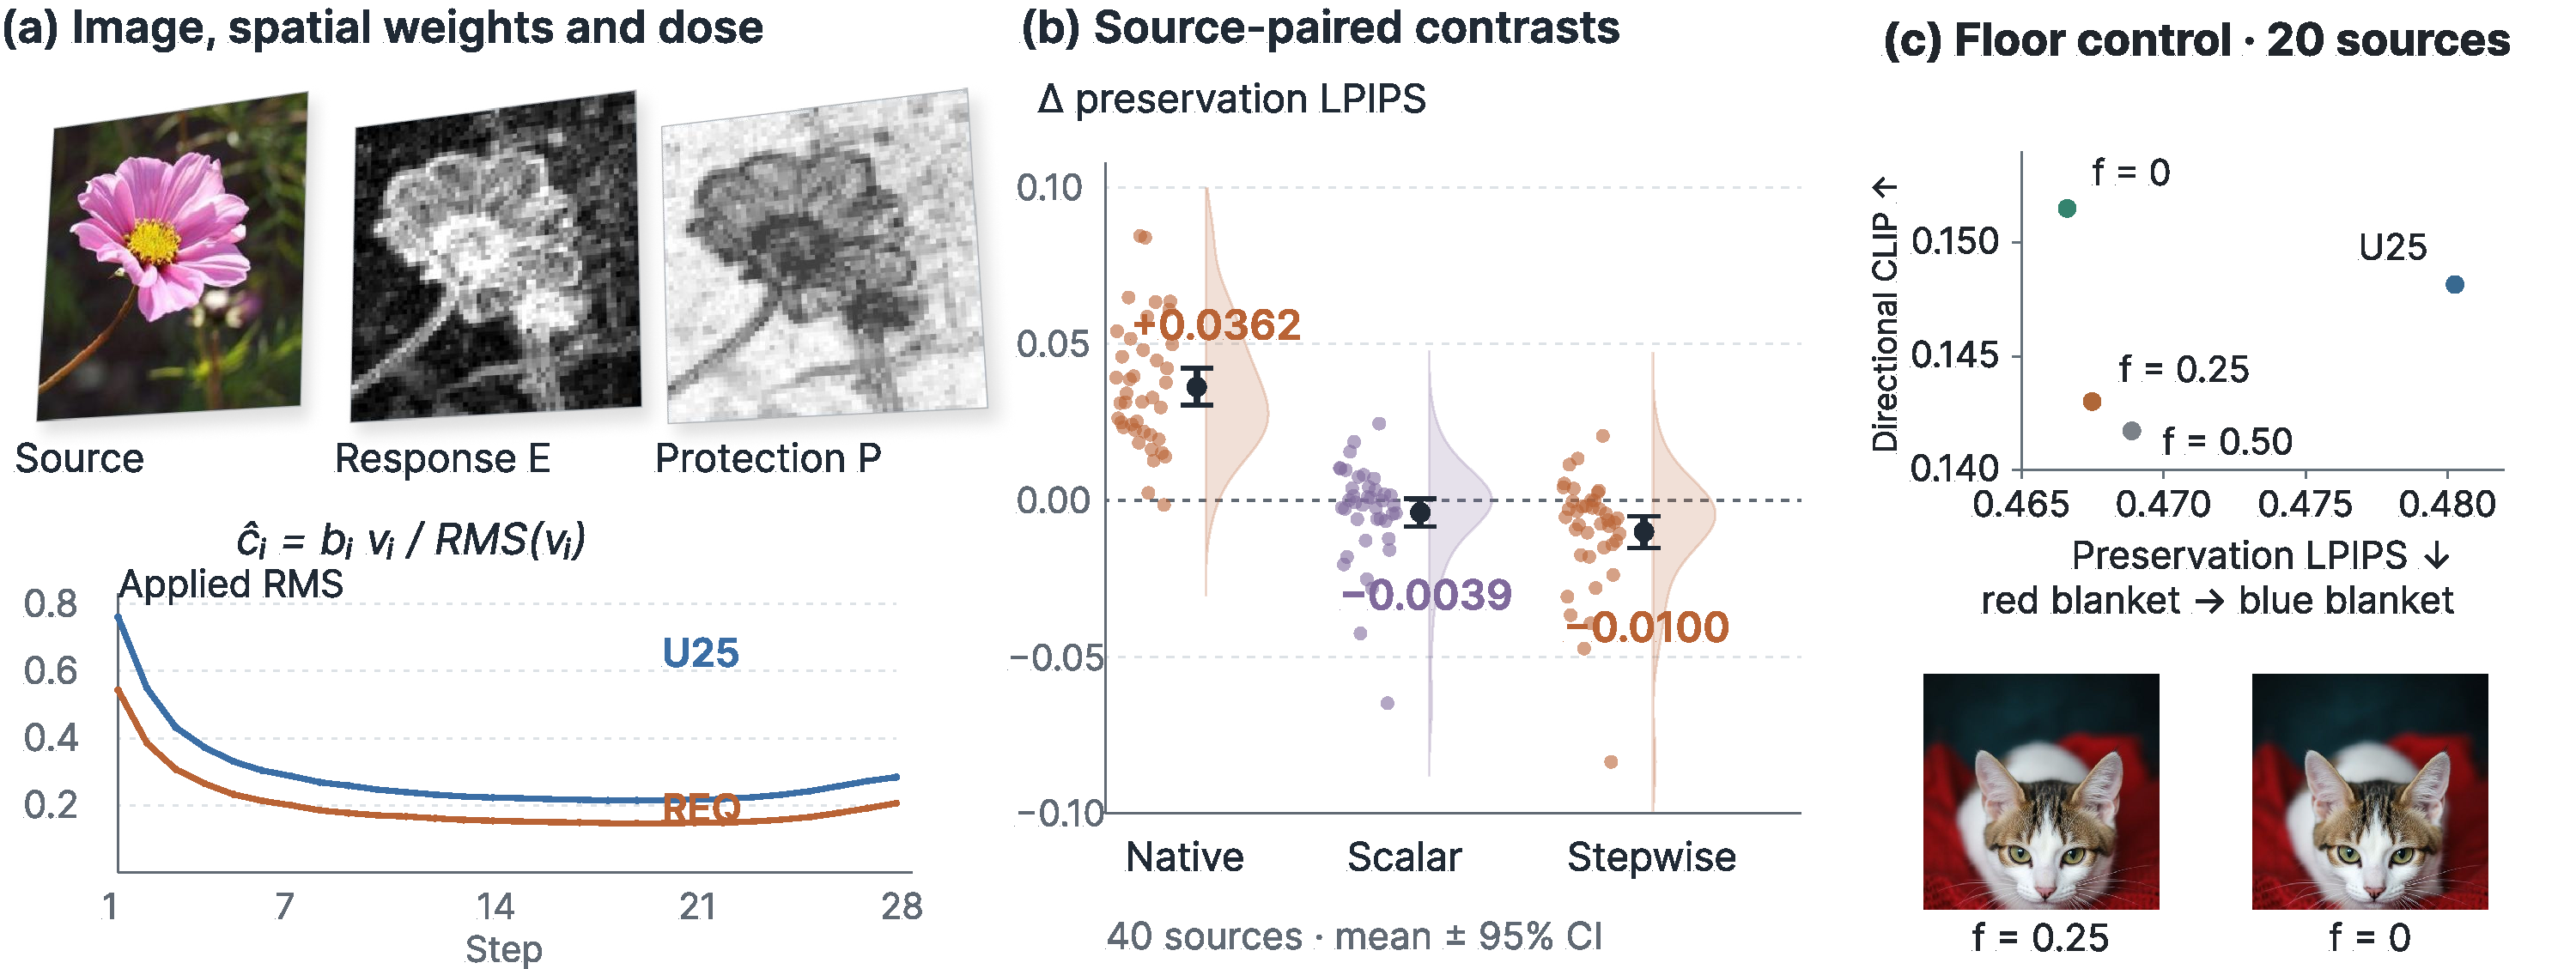
\includegraphics[width=\textwidth]{figures/evaluation_lens_v16.pdf}
\caption{(a) Flower source 117, perspective $E/P$ maps, and measured 28-step native U25/REQ correction-RMS profiles. (b) Paired native/SC/stepwise LPIPS contrasts over 40 sources, means, and source-bootstrap CIs; SC's CI includes zero. (c) Separate 20-source mean LPIPS/directional-CLIP points: U25 and floors $0/0.25/0.5$. Cat 94 retains a red blanket at both $f=0.25$ and $f=0$.}
\label{fig:legacy-lens}
\end{figure*}
\begin{figure*}[!t]
\centering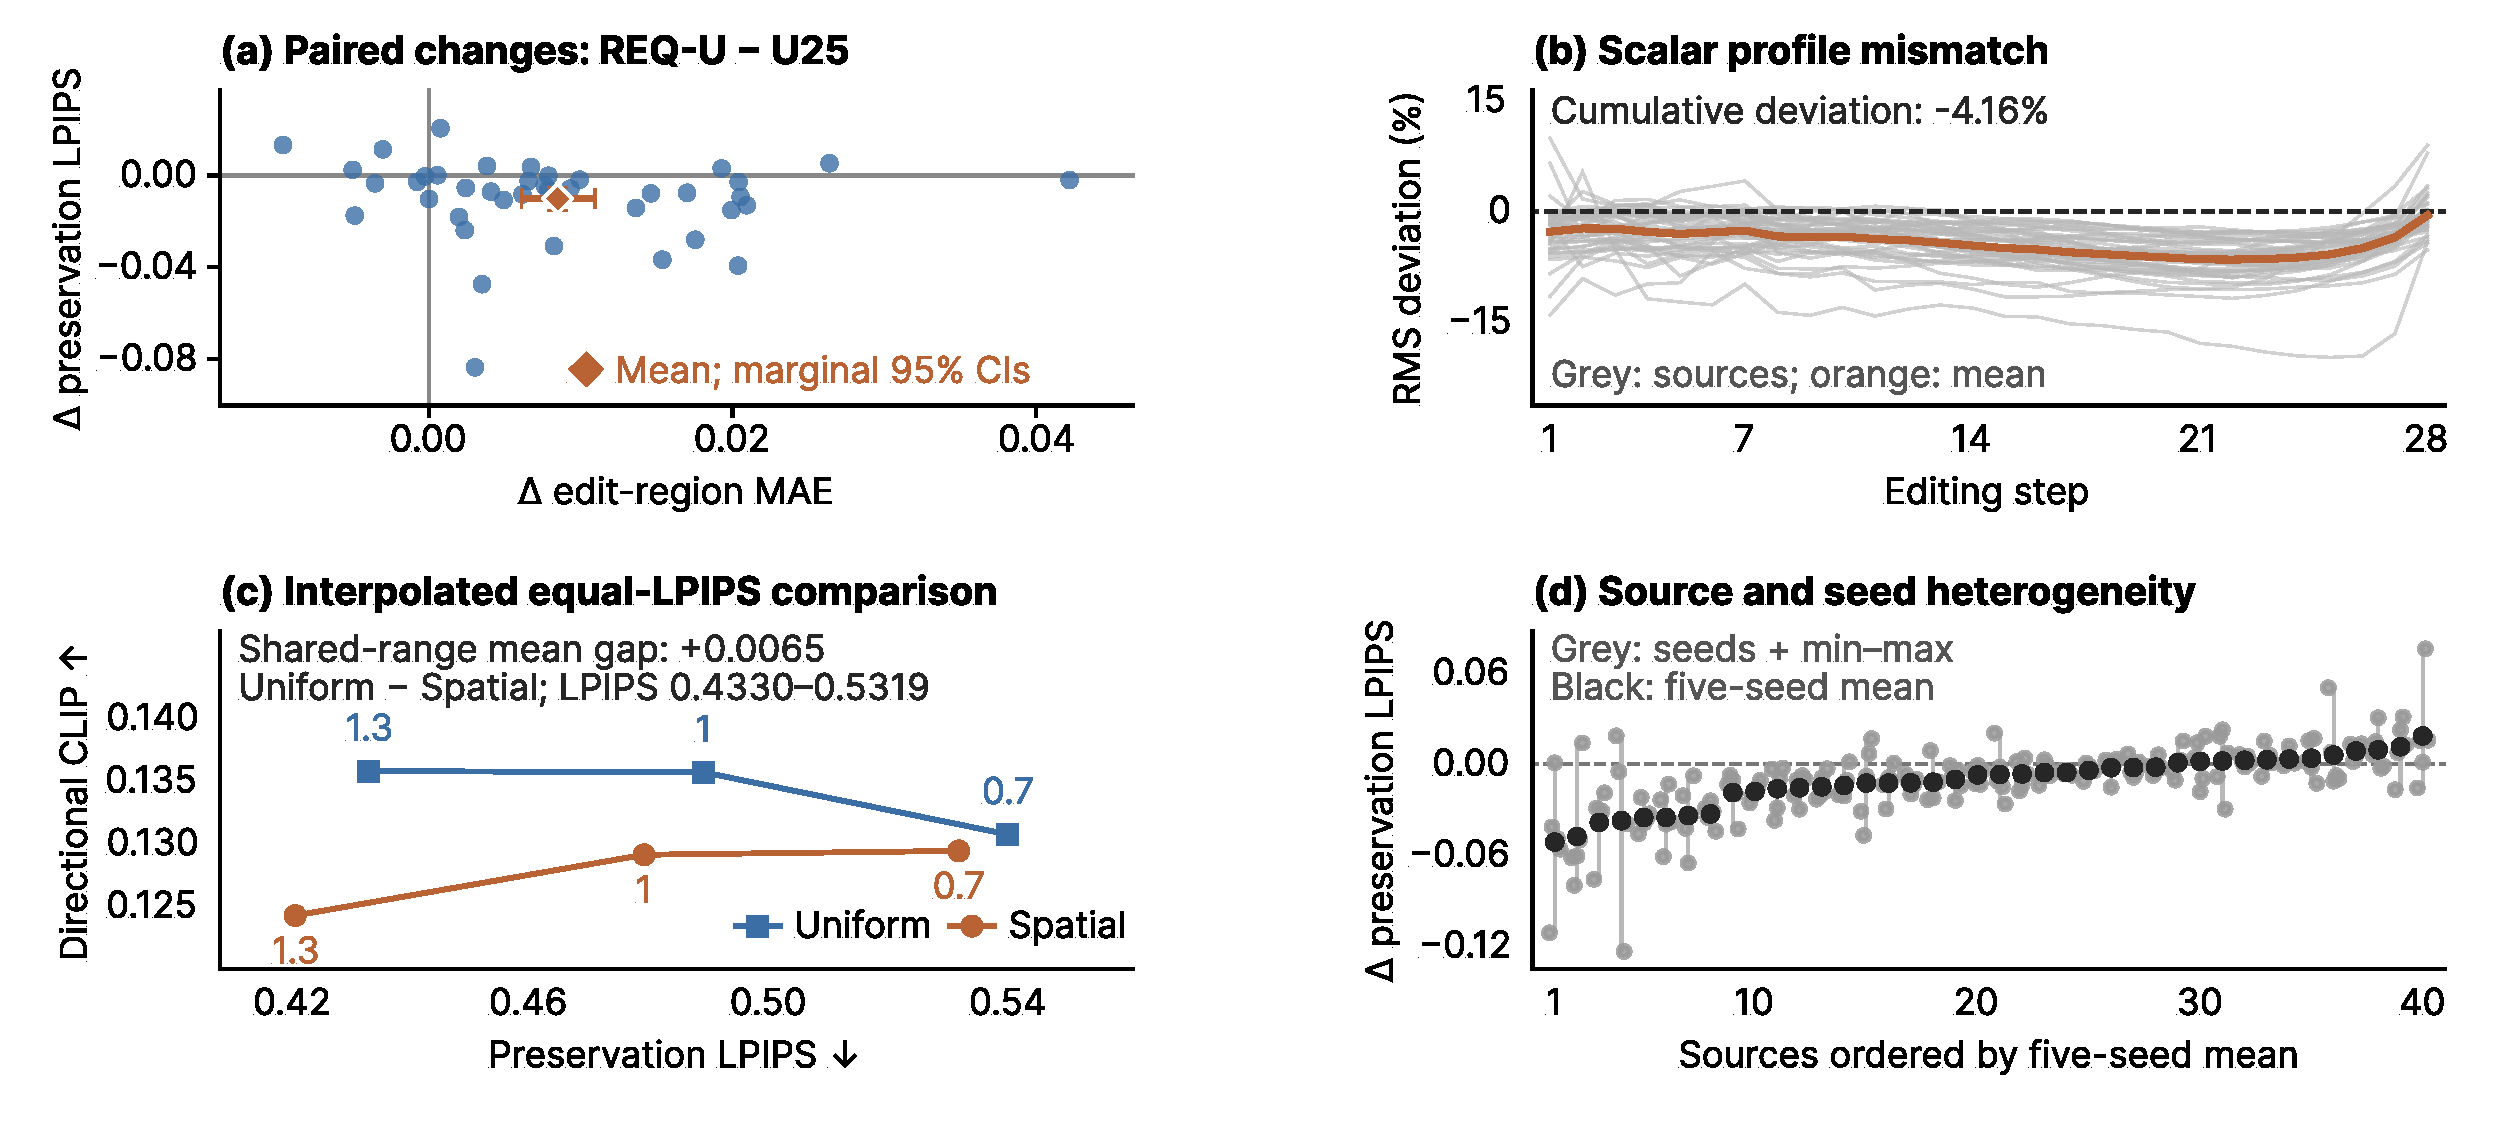
\includegraphics[width=\textwidth]{figures/evidence_summary_v16.pdf}
\caption{Calibration, attribution, and selection on the same 40 sources. (a) Source-paired REQ-U minus U25 differences, averaging seeds 0/17; the mean has marginal 95\% source-bootstrap intervals. Lower-right indicates more edit-region change with lower preservation LPIPS. (b) SC's actual RMS deviation from the target at each step: gray curves are source means over seeds 0/17, orange is their cohort mean. (c) Three observed scales per rule connected piecewise linearly; $+0.0065$ is the mean equal-LPIPS directional-CLIP gap over the shared range. (d) All five observed seeds per source: gray dots are seeds, black points are means, and bars span observed ranges.}
\label{fig:legacy-summary}
\end{figure*}
\begin{figure*}[!t]
\centering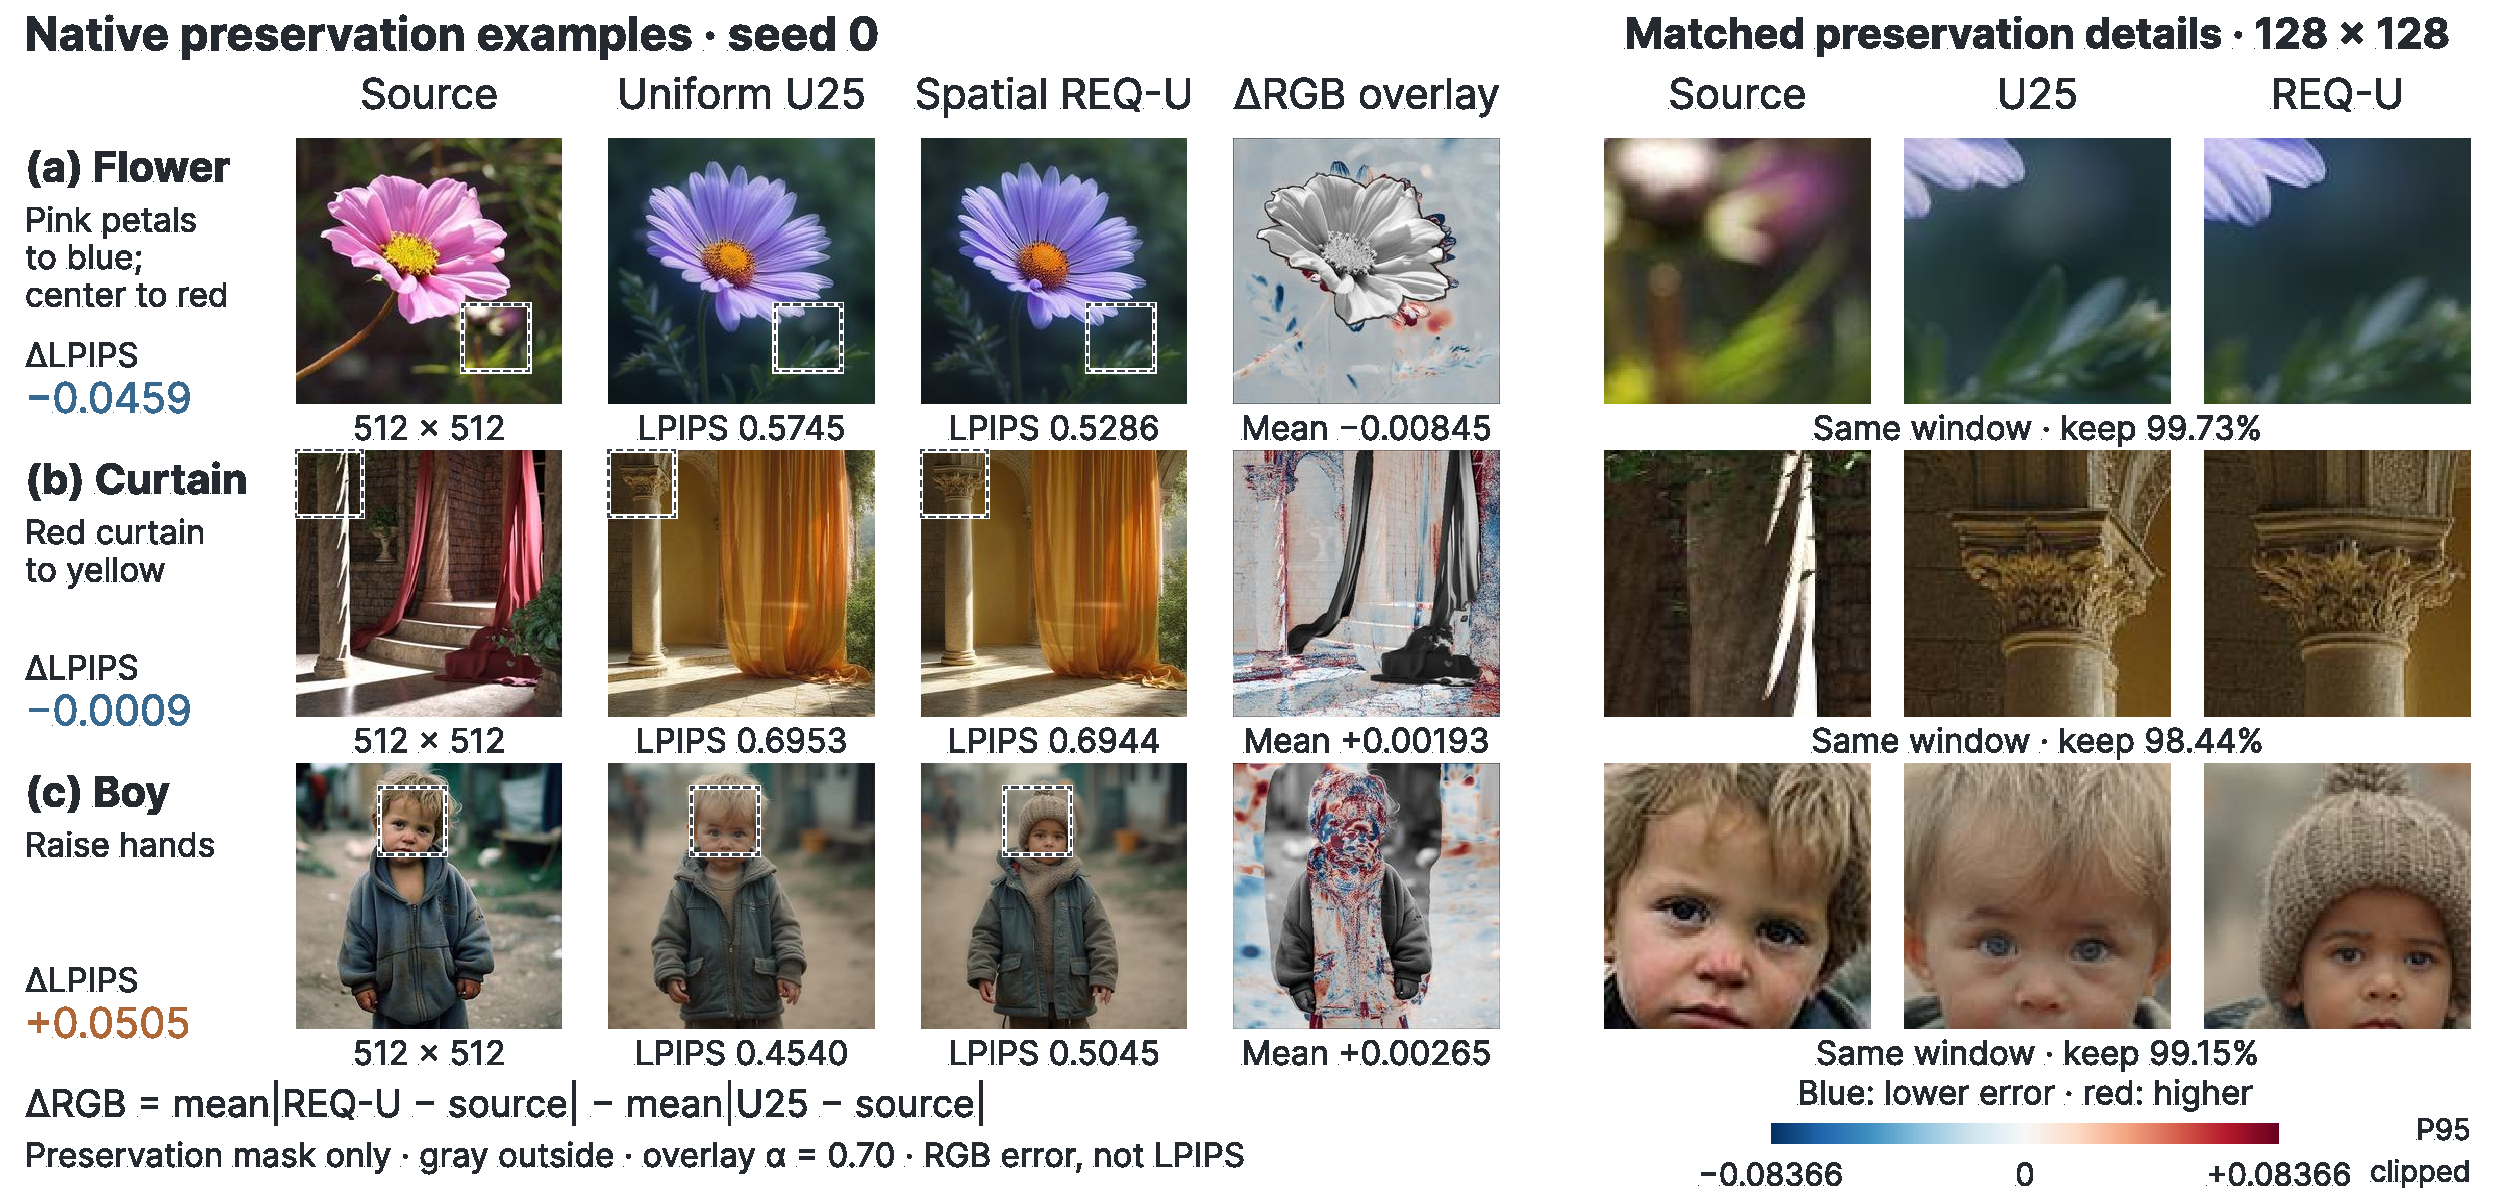
\includegraphics[width=\textwidth]{figures/native_error_v16.pdf}
\caption{Archived native $512\times512$ outputs; post hoc cases span favorable, near-zero, and unfavorable source-mean contrasts. Displayed LPIPS uses seed 0. Preservation overlays show signed RGB $[0,1]$ absolute-error differences (REQ-U minus U25), not LPIPS maps: $\alpha=0.70$, shared limits $\pm0.08366$ (pooled absolute-error-contrast P95; 4.98\% clipped). Blue favors REQ-U; red favors U25. Matched $128\times128$ crops with $\geq98\%$ preservation coverage are selected post hoc by maximum absolute error contrast. Images reuse original generations.}
\label{fig:legacy-native}
\end{figure*}
\paragraph{Figure evidence and selection.}
Figure~\ref{fig:legacy-lens} shows the source-correction interventions. Panel (a) presents the actual flower source 000000000117 at seed 0, its response map $E$, and protection map $P$ as perspective-arranged image slices, alongside the corresponding native 28-step U25 and REQ RMS profiles. The perspective arrangement is a display of the source and maps; the curves show recorded correction magnitudes. Panel (b) shows the paired source-level preservation-contrast distributions for native, one-shot SC, and stepwise comparisons on 40 sources, averaging seeds within source, with means and the cached marginal 95\% source-bootstrap intervals.

Panel (c) shows four joint-outcome means on the same fixed 20-source floor subset: $f=0$, $0.25$, $0.5$, and U25. Its native cat example uses source 000000000094, seed 0: the original R88 \texttt{REQ\_U} output at $f=0.25$ and the R91 \texttt{FLOOR000} output at $f=0$ share the same archived R88 U25 profile anchor. Both blankets remain red in these outputs; the pair illustrates the observed floor comparison, with the requested blanket-color change unsuccessful in both. The six measured $\beta\times$allocation points on 40 sources belong to Fig.~\ref{fig:legacy-summary}(c), separately from this 20-source floor comparison.

Figure~\ref{fig:protocol-flow} retains the detailed protocol previously shown in the main paper. Its source image, actual protection map, and two 28-step RMS curves use source 000000000117, seed 0. The curves retain the recorded U25 and REQ step values. Each replay arm evaluates its residual and target field at its own current state. The original editable TikZ asset, map array, and curve CSV document these computational inputs alongside the new evaluation-lens view.

The native qualitative inputs pair full $512\times512$ source, U25, and REQ-U images with signed RGB-error differences. The difference is $\Delta(x)=\frac{1}{3}\sum_c(|I_{\mathrm{REQ-U},c}(x)-I_{\mathrm{src},c}(x)|-|I_{\mathrm{U25},c}(x)-I_{\mathrm{src},c}(x)|)$, displayed on the preservation region with a common zero-centered scale; negative values indicate lower REQ-U pixel error. This is a pixel-error diagnostic, distinct from spatial LPIPS. In Fig.~\ref{fig:legacy-native}, the common limit is the pooled 95th percentile of absolute pixel contrasts and the overlay opacity is 0.70. Identical crop coordinates within each row maximize mean absolute contrast on a 16-pixel grid among windows with at least 98\% preservation coverage. The full crossed preview comparison remains in Fig.~\ref{fig:crossed-preview}; Fig.~\ref{fig:r92-native} adds the native SC comparison for the same three cases.

The quantitative figure inputs cover four questions. Paired image-change effects use all 40 sources after averaging seeds 0/17, with marginal source-bootstrap intervals for the cohort mean (Fig.~\ref{fig:paired-heterogeneity}). The SC profile panel shows realized stepwise RMS deviations from U25 (Fig.~\ref{fig:r92-scalar}). The interpolated equal-LPIPS comparison connects three measured scale points per rule on those 40 sources over the shared range defined in Section~\ref{sec:next-steps-20261106}. The seed summary retains all 200 source/seed contrasts: 14 sources are negative throughout, one positive throughout, and 25 change sign (Fig.~\ref{fig:r91-heterogeneity}). Negative favors REQ-U; observed seed ranges are distinct from confidence intervals. Floor settings form a separate 20-source comparison in Fig.~\ref{fig:r91}(c) and Table~\ref{tab:r91-floor-points}; they do not provide a floor-zero scale curve on the 40-source cohort.

The retained three-case crossed preview figure uses flower 000000000117, curtain 613000000001, and boy 522000000002 at seed 0. Their two-seed source-mean contrasts are $-0.039281$, $-0.0000993$, and $+0.020588$. Its unretouched $320\times320$ previews and actual $64\times64$ maps share display scales; the identical boy crop maps native $(160,32,128,128)$ to preview $(100,20,80,80)$ and has 99.19\% preservation coverage. The post hoc selection spans negative, near-zero, and positive effects, including incomplete flower-center and hand edits.

Figures~\ref{fig:qual} and \ref{fig:qual-maps} show six seed-0 cases: flower/curtain color changes, incomplete chair/blanket edits, streetlight-to-moon scene change, and inconsistent raised hands. The curtain case has a near-zero primary source contrast; the boy case favors U25 in source-averaged preservation LPIPS (REQ-U minus U25: $+0.0206$). Identically sized archived previews are unretouched. Brighter weights apply stronger correction. These examples illustrate outcomes rather than estimate their prevalence.

\paragraph{Native detail crops.}
Figure~\ref{fig:native-detail} shows mushroom and boy examples from native seed-0 outputs. The mushroom source has the second-largest preservation-LPIPS improvement among the 40 sources (REQ-U minus U25, averaged across seeds: $-0.0474$); the boy has the largest deterioration ($+0.0206$). These are post hoc selections from the source-level results. Identical $128\times128$ windows crop the source, U25, and REQ-U images. For the mushroom example, the sky window at $(x,y)=(256,64)$ was selected after viewing the outputs and contains 98.22\% official preservation pixels. For the boy, windows on a 16-pixel grid with at least 98\% preservation coverage are ranked by mean source-image grayscale gradient; the selected window at $(160,32)$ has 99.19\% coverage. The source-mean LPIPS contrasts summarize the entire preservation mask, rather than these selected crops.

\begin{figure}[!t]
\centering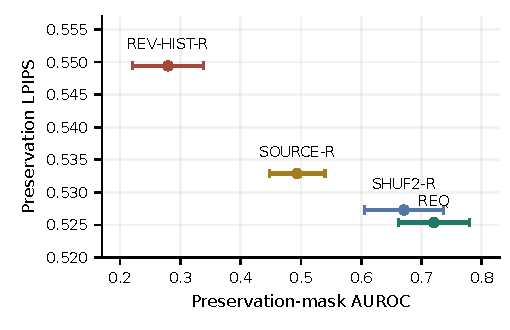
\includegraphics[width=\linewidth]{figures/map_alignment_supp.pdf}
\caption{Post hoc association between map-mask AUROC and preservation LPIPS for four constructions. Horizontal bars are marginal 95\% category-stratified source-bootstrap AUROC intervals. The points summarize constructed maps, not independently assigned levels of mask alignment.}
\label{fig:map-alignment}
\end{figure}

\begin{figure*}[!t]
\centering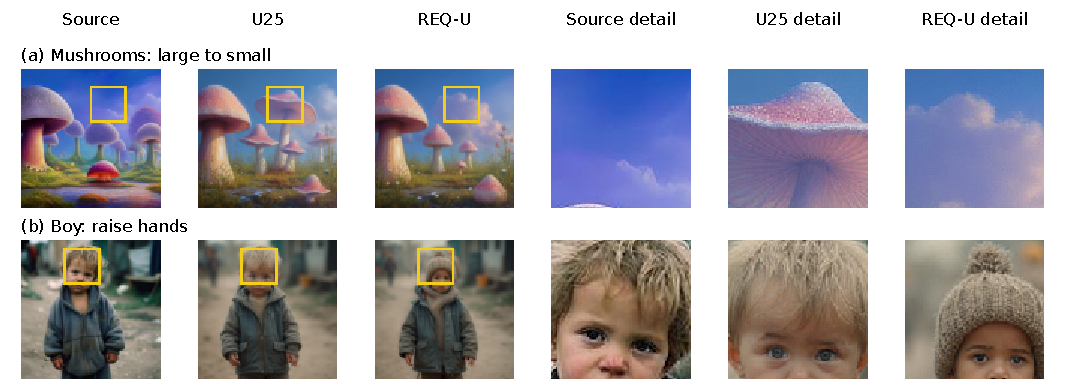
\includegraphics[width=.935\textwidth]{figures/native_preservation_detail.pdf}
\caption{Selected native seed-0 examples. The mushroom source (a) has the second-largest source-mean preservation improvement among 40 sources ($-0.0474$ LPIPS); the boy (b) has the largest deterioration ($+0.0206$). Neither output raises the boy's hands, visible in the full images. At least 98\% of each identical $128\times128$ crop lies inside the preservation mask. The sky crop in (a) was chosen after viewing outputs; (b) uses source gradients to show changes in the face region. Scores cover the full preservation mask.}
\label{fig:native-detail}
\end{figure*}

\paragraph{Paired image-change diagnostic.}
Figure~\ref{fig:paired-heterogeneity}(a) plots REQ-U minus U25 edit-region RGB MAE and preservation LPIPS for each source after averaging seeds 0 and 17. The mean MAE difference is $+0.00848$ (marginal 95\% CI $[0.00610,0.01095]$). The plotted intervals use 20,000 category-stratified paired source bootstraps with seed 88002; they describe two marginal intervals rather than a joint confidence region. Of 40 sources, 27 have larger edit-region MAE and lower preservation LPIPS, six increase both, four decrease both, and three have smaller edit-region MAE with higher preservation LPIPS. This is a post hoc description of actual pixel change, including unintended changes. Panel (b) ranks all 40 sources by their two-seed mean LPIPS contrast and shows both seed-specific effects; its connecting segments show the observed seed range, not uncertainty intervals. Per-output pixel measurements and LPIPS are in \path{cpu/pixels_by_output.csv} and \path{cpu/harmonized_lpips/R88_scores.csv}.

\begin{figure*}[!t]
\centering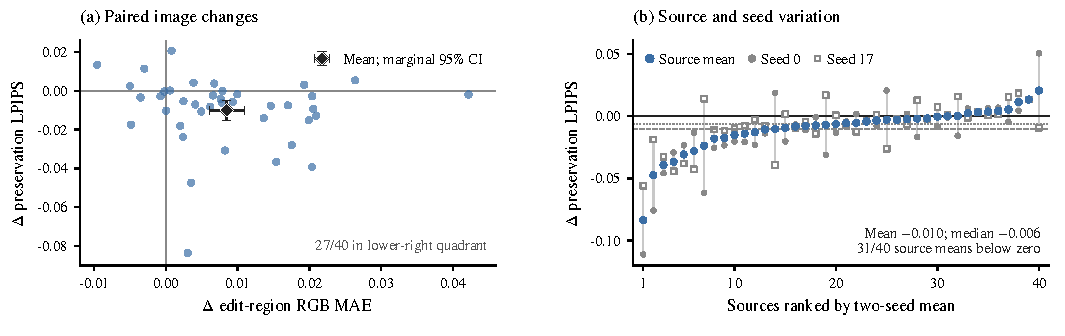
\includegraphics[width=\textwidth]{figures/paired_heterogeneity_v5.pdf}
\caption{REQ-U minus U25 across all 40 sources, with the full observed range retained. (a) Paired image changes, averaged over two seeds; the black diamond and bars show the mean and marginal 95\% source-bootstrap intervals. (b) Sources ranked by their two-seed mean preservation contrast. Blue points are source means; gray circles and open squares show seeds 0 and 17. Segments give observed seed variation. Dashed/dotted lines mark the cohort mean/median. Negative LPIPS differences favor REQ-U.}
\label{fig:paired-heterogeneity}
\end{figure*}

\paragraph{Mask-alignment diagnostic.}
Figure~\ref{fig:map-alignment} displays the four constructions covered by the archived alignment audit. Figure~\ref{fig:v19-corrector-controls} extends the original four-map diagnostic to the first shuffled donor with a reconstructed AUROC. No regression is fitted to these four means. Mask ordering, residual-energy alignment, and the spatial pattern of weights change together across constructions.


\begin{figure*}[!t]
\centering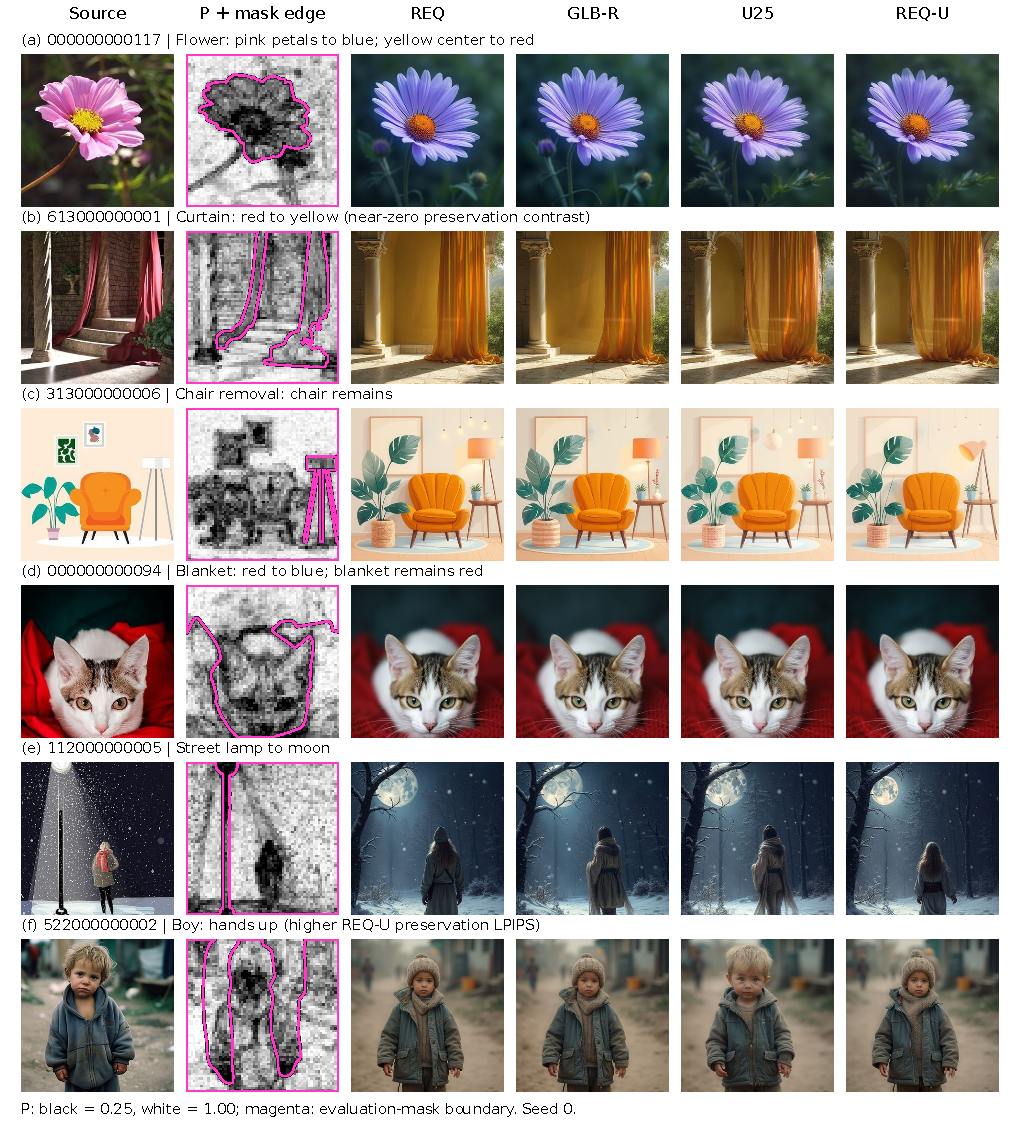
\includegraphics[width=\textwidth]{figures/qualitative_supp.pdf}
\caption{Source, protection map, and the four crossed direction/profile cells. Map interventions are shown separately in Fig.~\ref{fig:qual-maps}. Requests and selected preservation differences are displayed with the panels. All output images use seed 0. Rows show heterogeneous outcomes, including small metric differences and failed requested edits. Quantitative comparisons average both planned seeds.}
\label{fig:qual}
\end{figure*}
\begin{figure*}[!t]
\centering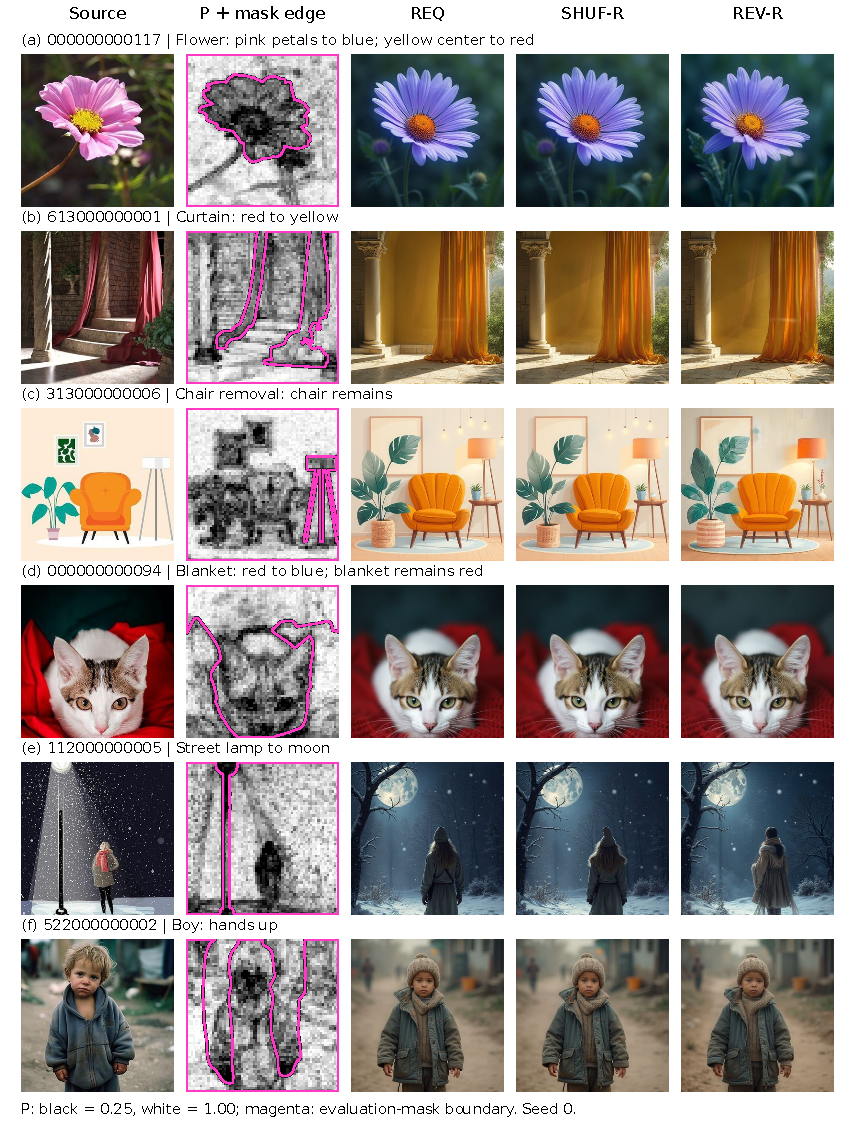
\includegraphics[width=0.76\textwidth]{figures/qualitative_supp_mapcontrols.pdf}
\caption{Map-control comparisons at the same request-origin profile: source, correct protection map, REQ, SHUF-R, and REV-R. Inspect changes outside the requested object as well as whether the edit occurred. All images use seed 0; these rows are illustrations, not preference labels.}
\label{fig:qual-maps}
\end{figure*}

\begin{figure*}[!t]
\centering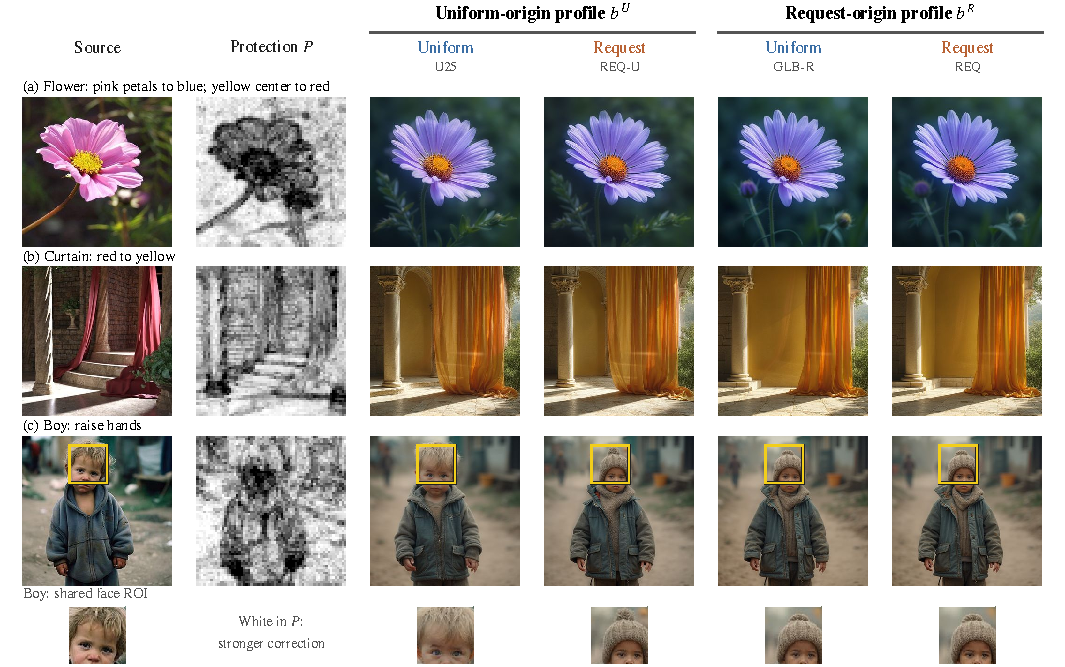
\includegraphics[width=\textwidth]{figures/qualitative_matrix_v10.pdf}
\caption{Full crossed comparisons, seed 0. White in actual $P$ means stronger correction. Post hoc flower, curtain, and boy cases span negative, near-zero, and positive two-seed source-mean preservation contrasts ($-0.0393,-0.0001,+0.0206$). RGB panels are archived $320\times320$ previews, with an identical boy-face crop; metrics use native outputs. Incomplete flower-center and hand edits show why preservation alone is insufficient.}
\label{fig:crossed-preview}
\end{figure*}

\section{Reproducibility}\label{sec:reproducibility}

\subsection{Native coverage and record identity}
The primary and scale/map studies (R88/R89) contain 480 and 640 outputs respectively. Of their 1,120 recorded output digests, 160 matched a retained native PNG; 960 have score records only. The seed/map/floor study (R91) contributes 720 scientific outputs, and the scalar study (R92) adds 80, for 1,920 distinct scientific runs on the restoring cohort. The four extra seed-0 checks repeat earlier outputs. Seeds 1, 2 and 3 each cover all 40 sources in each of REQ, GLB\_R, REQ\_U and U25. Thus both fixed-profile contrasts can be rescored on all three added seeds; on the original two seeds only the uniform-profile pair has complete native files.

The six per-output score tables in \path{cpu/harmonized_lpips/} retain SHA-256 identifiers for output, source and mask. Across SAM, restoring and DirectEdit the 1,964 rescored rows have 1,960 distinct output digests. \path{evidence/historical_native_coverage.csv} lists all early output hashes and retrieval flags. \path{evidence/native_counts.csv} gives arm and seed counts; \path{evidence/provenance.json} records archive digests, the SAM evaluator and mask-manifest hashes, CPU versions, LPIPS weight digests and the original-score verification errors.

All six planned automatic outcomes for the primary and scale/map studies are complete. The original R88 evaluation CSV additionally contains native REQ edit-region MAE (\texttt{object\_mae}): all 80 records have status OK, with mean 0.164571 after seed averaging within 40 sources. For the 160 U25/REQ-U entries shared with the later reconstruction, the same field agrees within $10^{-16}$. The corresponding SC minus native REQ edit MAE is $-0.016425$. Table~\ref{tab:r92-results} identifies the recovered source of that cell. Seed/floor/scalar evaluations retain LPIPS, CLIP and regional MAE.


\paragraph{What to run.}
Run \path{reproduce.py} for restoring contrasts, SAM constant-gain recovery, selectivity and four- and five-setting MRC. Use \path{analysis/v20_mrc/reproduce_mrc.py} for both editors' response sensitivities and \path{SAM_scan/reproduce.py} for the original scorer and 6,500 projection-step records. \path{SAM_scan/control/} and \path{SAM_scan/data/protocol.json} supply the operator and settings. The early study archive contains generator and evaluator code, step summaries and maps. The compact ZIP includes source-level measurements and a four-cell profile. Two early metadata files were unavailable (\path{runtime_base/results/evaluation_config.json} and \path{run/identity.json}).

The two-seed native path estimates and the cohort-mean equal-LPIPS interpolation are also retained as archived aggregates. \path{analysis/history/supp_history_recovered.json} identifies their original records, the 80 native REQ trajectories and DirectEdit extrapolations. The three-setting within-source analysis can be reaggregated separately from \path{source_correction_and_blending/three_scale_points.csv}.

\subsection{Implementation and evaluation metadata}
The restoring protocol specifies FLUX.1-dev revision \path{3de623fc3c33e44ffbe2bad470d0f45bccf2eb21}; CLIP ViT-L/14 uses \path{32bd64288804d66eefd0ccbe215aa642df71cc41}; DINOv2-base uses \path{f9e44c814b77203eaa57a6bdbbd535f21ede1415}. Snapshot identities and processor calls are archived; processor configuration files are outside the compact package. DirectEdit follows official commit \path{26b04bf576bfb83204bea619ae411d075faec99e}, with BF16 network evaluation and FP32 integration in place of the example's FP16. The archived evaluator uses LPIPS 0.1.4. Local evaluation uses FP32 on CPU with autocast off, PyTorch 2.11.0 for seed/floor/scalar evaluation, and Transformers 4.55.4. Scalar calibration reuses the seed study's recorded FLUX model inventory.
For R92, the audit names the expected historical FLUX revision above and records \path{revision_directory_matches=false} for the local model binding. Its tensor inventory agrees with R91 in names, headers and lengths. A full generator-weight payload digest was unavailable for this comparison.

Caching reuses source encoding, prompt embeddings, inversion states, reference motion, probes, and compatible source memory; each arm computes its residual at its own edited state. The primary equivalence check covers all six arms on one source/seed and records identical outputs. Four seed-study checks repeat U25/REQ-U at seed 0 on sources 000000000094 and 822000000006, reproducing native RGB exactly; maximum score differences are $5.96\times10^{-8}$ (preservation LPIPS), $8.94\times10^{-8}$ (target CLIP), and $2.46\times10^{-7}$ (directional CLIP).

The seed/map/floor study and checks use 52,368 incremental evaluations and 7.552 synchronized job-hours; maximum relative RMS error across 13,496 replay steps is $2.21\times10^{-7}$. Scalar calibration has 2,240 steps, 7,760 evaluations (97/output), and 4,000.79 synchronized job-seconds (1.111 hours). All 724 seed-study/check runs and 80 scalar runs completed without recorded generation failures. Timings exclude loading and evaluation; main and scale/map costs appear in Tables~\ref{tab:cost} and \ref{tab:r89-cost}.


The exploratory REML fits did not converge. The reported intervals use source resampling.

\paragraph{Archived model ratings.}\label{sec:model-judge80}
One DeepSeek-V4.1-Flash pass viewed randomized REQ-U/U25 pairs (40 sources, seeds 0/17; $512\times512$ images displayed in an approximately 390-pixel panel). Background preference tied on 80/80 pairs and instruction labels on 78/80, including 20 joint failures and five joint uncertain calls. Both discordant instruction labels favored REQ-U. This pass had no human calibration; the exact API settings and complete transcript were unavailable.

\subsection{Scope of the paired evidence}
The source-correction comparisons condition on 40 sources and a fixed FLUX editor, with additional seeds measured on those same sources. The SAM experiment conditions on 50 sources and one generation seed, with backgrounds measurable on 42. DirectEdit uses 20 of the source-correction sources with its own mask and blending rule. The different operators and regional scoring procedures each define their own contrast.

The reported outcomes are automatic metrics and annotated examples. No human evaluation was conducted. Alternative regional RMS controls and calibration of a scalar to the realized total on its own rollout remain distinct, unmeasured interventions.

\subsection{AI assistance}
OpenAI Codex assisted drafting and language revision throughout the main paper and supplement, development of analysis code, and preparation of data figures. The authors are responsible for the analyses and final content.


\section{Reading the Comparisons}\label{sec:decision-guide}
Compare configurations over each image's shared response range. Attribute allocation effects by naming the gated term and crossing the two native profiles. Report a calibrated scalar's realized magnitude alongside its output scores. For external blends, identify coefficients and sources outside the convex range (Section~\ref{sec:external}).

\begin{thebibliography}{7}
\bibitem{cui2026sam}
H. Cui, R. Chen, T. Luo, T. Guo, Z. Qin, and J. Wang, 
``SAM-Flow: Source-anchored masked flow for training-free image editing,'' arXiv:2606.06228, 2026.
\bibitem{kulikov2025flowedit}
V. Kulikov, M. Kleiner, I. Huberman-Spiegelglas, and T. Michaeli,
``FlowEdit: Inversion-free text-based editing using pre-trained flow models,'' in \emph{Proc. ICCV}, 2025, pp.~19721--19730.
\bibitem{yang2026directedit}
D. Yang and M. Ye,
``DirectEdit: Step-level accurate inversion for flow-based image editing,''
in \emph{Proc. ICML}, vol. 306, 2026, pp. 146750--146765.
\bibitem{li2026veloedit}
Z. Li et al., ``VeloEdit: Training-free consistent and continuous instruction-based image editing via velocity field decomposition,'' arXiv:2603.13388, 2026.
\bibitem{zhan2026decflowedit}
Z. Zhan, C. Wang, J. Chen, C. Chen, S. Lyu, Z. Zheng, and D. Chen, ``DecFlowEdit: Self-localized flow-based image editing via guidance decoupling,'' arXiv:2609.34237, 2026.
\bibitem{li2026asg}
Z. Li et al., ``Attention-scoped guidance: Training-free spatial control for image editing,'' arXiv:2609.37492, 2026.
\bibitem{xie2026guidancematters}
D. Xie et al., ``Guidance matters: Rethinking the evaluation pitfall for text-to-image generation,'' in \emph{Proc. ICLR}, 2026.
\end{thebibliography}
\end{document}
